


\documentclass[12pt]{article}
\usepackage{natbib}
\usepackage[flushleft]{threeparttable}
\usepackage{longtable}
\usepackage{bm}

\usepackage{caption}


\captionsetup[figure]{font=normalsize, labelfont=bf}






\usepackage{listings}
\usepackage[english]{babel}
\usepackage[utf8]{inputenc}
\usepackage[dvips]{graphicx}
\usepackage{amsmath,amsthm,amssymb,tipa,dsfont,mathtools,mathrsfs,here,titlesec,fancyhdr}
\usepackage{anysize}
\usepackage{subfigure}
\usepackage{color}
\usepackage{enumerate}
\usepackage{booktabs}
\usepackage{rotating}
\usepackage{parskip} % to avoid // 
\usepackage[hidelinks]{hyperref}
\usepackage{url}
\usepackage{multirow}
\renewcommand{\qedsymbol}{\rule{0.7em}{0.7em}}
\usepackage{comment} % begin{comment} to comment large sections
\usepackage[font=scriptsize]{caption}
\usepackage{rotating} % to rotate tables 
\usepackage{tikz}
\usetikzlibrary{shapes,decorations,arrows,calc,arrows.meta,fit,positioning}
\tikzset{
	-Latex,auto,node distance =1 cm and 1 cm,semithick,
	state/.style ={ellipse, draw, minimum width = 0.7 cm},
	point/.style = {circle, draw, inner sep=0.04cm,fill,node contents={}},
	bidirected/.style={Latex-Latex,dashed},
	el/.style = {inner sep=2pt, align=left, sloped}
}

\definecolor{Grey}{RGB}{150, 150, 150}
\definecolor{PPblue}{RGB}{0,114,198}
\definecolor{VOXblue}{RGB}{0,114,198}
\definecolor{PSOEred}{RGB}{232,0,0}
\definecolor{UPred}{RGB}{232,0,0}
\newcommand{\sym}[1]{\rlap{#1}}

\definecolor{mypink}{rgb}{0.858, 0.188, 0.478}
\definecolor{myorange}{rgb}{1.0, 0.49, 0.0}
\definecolor{mypurple}{rgb}{0.6, 0.4, 0.8}
%\usepackage[colorlinks=true,linkcolor=blue,citecolor=blue,hyperfootnotes=false]{hyperref} 
\hypersetup{
	colorlinks,
	citecolor=blue,
	linkcolor=mypink,
	urlcolor=mypurple}
%Els comandaments següents són per a linkejar (han d'estar al final de tots els usepackage)
%\usepackage[colorlinks]{hyperref}%aquests paquets s'utilitzen per a poder linkejar coses.
%\hypersetup{citecolor=red}
%\hypersetup{linkcolor=red}
%\hypersetup{urlcolor=red}
%\usepackage{cleveref}%aquest també.

\usepackage[T1]{fontenc} % for porper quotation marks 
\PassOptionsToPackage{svgnames}{xcolor}
\usepackage{pgfplots}


\usepackage{tcolorbox}
\usepackage{lipsum}
\tcbuselibrary{skins,breakable}
\usetikzlibrary{shadings,shadows}
\newenvironment{myblock}[1]{%
	\tcolorbox[beamer,%
	noparskip,breakable,
	colback=LightBlue,colframe=DarkBlue,%
	colbacklower=DarkBlue!75!LightBlue,%
	title=#1]}%
{\endtcolorbox}

\usepackage{tikz}
\usetikzlibrary{shapes,decorations,arrows,calc,arrows.meta,fit,positioning}
\tikzset{
	-Latex,auto,node distance =1 cm and 1 cm,semithick,
	state/.style ={ellipse, draw, minimum width = 0.7 cm},
	point/.style = {circle, draw, inner sep=0.04cm,fill,node contents={}},
	bidirected/.style={Latex-Latex,dashed},
	el/.style = {inner sep=2pt, align=left, sloped}
}














\renewcommand{\baselinestretch}{1.2} %separació entre linies
\marginsize{2.3cm}{2.3cm}{1cm}{2cm} %Margens


%ací definim els colors que anem a gastar
\definecolor{secction}{rgb}{0.62,0.31,0.00}
\definecolor{subsection}{rgb}{0.33,0.00,0.33}
\definecolor{mygreen}{RGB}{28,172,0}


%S'utilitza per a insertar programes de forma més professional
%\lstset{language=Matlab,numbers=left,frame=single,title=\lstname}
\lstset{language=Matlab,%
    %basicstyle=\color{red},
    breaklines=true,%
    morekeywords={matlab2tikz},
    keywordstyle=\color{blue},%
    morekeywords=[2]{1}, keywordstyle=[2]{\color{black}},
    identifierstyle=\color{black},%
    %stringstyle=\color{mylilas},
    commentstyle=\color{mygreen},%
    showstringspaces=false,%without this there will be a symbol in the places where there is a space
    numbers=left,%
    numberstyle={\tiny \color{black}},% size of the numbers
    numbersep=9pt, % this defines how far the numbers are from the text
    emph=[1]{for,end,break},emphstyle=[1]\color{blue}, %some words to emphasise
    %emph=[2]{word1,word2}, emphstyle=[2]{style},
}

\usepackage[colorinlistoftodos,textwidth=3cm]{todonotes}
\newcommand{\todoINFO}[1]{\todo[color=blue!25]{INFO: #1}}
\newcommand{\todoIMPORTANT}[1]{\todo[color=red!25]{IMPORTANT: #1}}
\newcommand{\todoREV}[1]{\todo[color=green!25]{REVIEWED: #1}}
%Aquí redefinimos los comandos teorema, nota, etc... para que sea más fácil de escribir. Lo que está entre corchetes "[,]" es para que enumere los teoremas en función de la sección, si se quita, lo enumera sobre el total.
\theoremstyle{plain}
\newtheorem{teo}{Theorem}[section]
\newtheorem{prop}{Proposition}[section]
\newtheorem{exe}{Exercise}
\theoremstyle{definition}
\newtheorem{defi}{Definition}[section]
\newtheorem{nota}{Note}
\DeclarePairedDelimiter\abs{\lvert}{\rvert}%
\DeclarePairedDelimiter\norm{\lVert}{\rVert}%
%abreviatures dels comandaments "begin/end". Es una chorradita por no escribirlo todo, puedes usarlo o no.
\newcommand{\be}{\begin{exe}}
\newcommand{\ee}{\end{exe}}
\newcommand{\bt}{\begin{teo}}
\newcommand{\et}{\end{teo}}
\newcommand{\bd}{\begin{defi}}
\newcommand{\ed}{\end{defi}}
\newcommand{\bn}{\begin{nota}}
\newcommand{\en}{\end{nota}}
\newcommand{\bp}{\begin{proof}}
\newcommand{\ep}{\end{proof}}
\usepackage{accents}
\newcommand{\ubar}[1]{\underaccent{\bar}{#1}}

%abreviatures de símbols. Esto en realidad no lo utilizo nunca, pero si te acostumbras es más cómodo.
\newcommand{\e}{\exists}
\newcommand{\fa}{\forall}
%\newcommand{\iff}{\Leftrightarrow}

%Comandaments utilitzats per a donar un millor estil a les pàgines (la xorradeta de la linia de dalt)
\usepackage{fancyhdr}
\pagestyle{fancy}
\lhead{}
%\rhead{Luis Ignacio Menéndez García}
%\renewcommand{\footrulewidth}{0.3pt}

\renewcommand{\headrulewidth}{0pt}   % no line under the header
\renewcommand{\footrulewidth}{0pt}   % no line above the footer


%here we use a new command for the figures titles
\newcommand*{\figuretitle}[1]{%
	{\centering%   <--------  will only affect the title because of the grouping (by the
		\textbf{#1}%              braces before \centering and behind \medskip). If you remove
		\par\medskip}%            these braces the whole body of a {figure} env will be centered.
}

\DeclareMathOperator*{\E}{\mathbb{E}}
\DeclareMathOperator*{\R}{\mathbb{R}}
\DeclareMathOperator*{\Lag}{\mathscr{L}}
\DeclareMathOperator*{\contr}{\Rightarrow\Leftarrow}
\DeclareMathOperator*{\convprob}{\overset{p}{\to}}
\DeclareMathOperator*{\convas}{\overset{a.s.}{\to}}
\DeclareMathOperator*{\convd}{\overset{d}{\to}}
\DeclareMathOperator*{\impose}{\stackrel{!}{=}}



%change colorlinks=false if you don't wan't any hyperlinks to have color

%cmd+n to open a new wnvironment for equation see macros in options of texstudio



%\usepackage[paperwidth=275.9mm, paperheight=279.4mm]{geometry} 
\usepackage{afterpage}
\usepackage{calligra}
\newcommand{\share}{\mbox{\calligra{S}}}

\title{The Impact of Political Campaigns on Demand for Partisan News}
\author{Luis  Menéndez \thanks{Universitat Autònoma de Barcelona, CSIC and Barcelona School of Economics}} %omit the footnote and thanks if needed
\date{\today}

\begin{document}
	\maketitle
	
	\begin{abstract}
		

		
		

		
		Political polarization in news consumption has recently gained attention, yet policies to limit it are hard to evaluate. This paper introduces a novel, self-collected dataset on Spanish prime-time TV news—the dominant source of political information in Europe. I identify stories minute-by-minute and match them across newscasts to compare editorial treatment. Combining machine-learning methods with large language models, I classify the partisan slant of each story and use the resulting data to document changes in news coverage during the 2023 presidential campaign. I then match these data to high-frequency audience-meter records and estimate a structural random-coefficients demand model to understand how outlets compete in coverage and tone of news about different political parties. Exogenous shifts in the news landscape that constrain channels’ ability to shape content serve as instruments for slant and allow me to recover demand preferences. I find significant evidence of affective polarization only after the election campaign begins. Given the demand estimates, I back out outlets’ content preferences from a horizontal-differentiation game. Finally, I run counterfactual simulations to assess the effects of adopting the proportional-airtime rules enforced in other European countries but not in Spain. The framework offers a tractable tool for evaluating media policies aimed at content fairness or fighting misinformation.
		
		
		
	\end{abstract}
	
	


	
	
	
	
	
	
	
	\clearpage
	
	
	
	\section{Introduction }
	
	

Media plays a crucial role in disseminating information and can influence voting outcomes \citep{Zhuravskaya2020}. Consequently, policymakers often regulate media markets to ensure informational plurality during political campaigns.   \footnote{In Italy, the Par Condicio law mandates equal time and space on television, radio, and press for all political actors during campaign periods. Similarly, the Conseil supérieur de l’audiovisuel applies a similar rule to both private and public broadcasters in France. Spanish "Ley de Medios" recommends equal time rule policies only for the public broadcaster Televisión Española (TVE).}

However, assessing the effectiveness of these regulations requires understanding how viewers respond to the content they consume. Previous research has demonstrated media’s influence on voting behavior during political campaigns . This issue is particularly relevant in Spain, where political polarization ranks among the highest in Europe, according to recent surveys \citep{edelman_trust_2023}. Notably, affective polarization has increased significantly during our sampling period, raising the question of whether citizens’ political news consumption patterns reflect similar trends.


In this paper I estimate the extent of confirmation bias and polarization in the demand forpolitical content and how this changes with political campaigns. To this purpose I make use of a unique dataset that comprises both the demand and the supply of political content in Spainish TV news. On the demand side, I use high frequency audimeter data; thereby addressing some of the well-known limitations of survey-based studies \citep{prior}. For the supply of content, I built a unique text dataset and use Natural Language processing and LLMs to classify the political tone of the news. This classification is robust to previous methods used in the literature but allows me to do a more flexible specification where I can distinguish the airtime devoted to each party-tone on a given day. 

By exploiting geographical variation in the audience demand, I allow the preferences for content to differ by demographics- i.e political ideology. This allows me to study polarization in the news consumption. 

I document the market equilibrium and the endogeneity that arises from it. More right wing outlets also match woth more right wing viewers and viceversa. This makes the content offered by a channel an equilibrium outcome of a differentiation game and poses endogeneity concerns in the demand estiamtion. I propose a novel identification strategy that allows me to track supply shocks in the content offered by the outlets. Specifically, I obtain all the sotires that have been produce in Spain by the largest Spanish news agency which supplies the content to all the outlets in my sample. I see this as a proxy for the "news landscape" available for the outlets to produce. The mechanism is then intuitive: Outlets are in a long run equilibrium in the differentiation game and want to stick to their ideological positions. Daily news shocks limit what they can produce and thus make some days more or less favorable for a given outlet depending on the nature of the stories available. My descriptive evidence confirms this intuition: Right (left) wing channels increase their production of stories more whenever the pool of favorable right wing stories is higher. 



My findings align with previous research on polarized news consumption in the U.S. \citep{Peterson2017Echo}. In the pre-campaign period, there is no systematic asymmetry in political content demand between right- and left-leaning audiences, even when controlling for voting intentions or channel-specific preferences. However, during political campaigns, I find evidence of affective polarization: right-leaning viewers increasingly seek negative coverage of the opposing left-wing party while favoring more positive coverage of their own. This shift in demand coincides with a homogenization of political stances across outlets. Moreover, my results suggest a partisan divide in the overall preference for political content. XXX


In the last part of the paper I model and estimate the news production of the outlets making use of the demand estimates. Outlets play a pure horizontal differentiation game (no prices) and choose the slant of the day to maximize their viewership. Costs come from producing content as a function of the inputs they have available on that given day. Key for identification is the timing of the game. By using the initial audience of the day (i.e before viewer's have been exposed to the actual content); I avoid simultaneity issues as audience reactions follow content chosen since the later can't be modified life. 

I estimate the cost parameters and solve the new equilibrium under different counterfactual scenarios evaluating the impact of recently debated regulations such as the proportional airtime rule. 


This study contributes to the literature on political preferences in media consumption by leveraging exogenous variation in the news landscape to identify political preferences. Notably, my approach relies on unsupervised classification techniques that streamline political categorization. To the best of my knowledge, this is the first paper to examine preferences for political content during campaign periods while explicitly addressing the endogeneity in content supply.








%My analysis focuses on how TV news demand changes during political campaign periods. Previous research has shown that the rise of soft news has contributed to declining interest in political news \citep{patterson2000doing}. Consistent with \cite{gambaro2021revealed}, my findings suggest that periods in which political content is mixed with other types of programming encourage greater audience engagement with politics.

%I then investigate the extent of polarized news consumption. Using different machine learning methods, I desing a pipeline that extracts the daily news videos, converts the audio into text and splits the different stories of the day. This methodology allows me to build comparative statics on tone and duration of the same story treated by different outlets on a given day. Using text analysis techniques, I control for the political stance and duration of news stories \citep{puglisi_review}. Specifically, I make use of Large Language Models (LLMs) by inputting all stories into ChatGPT-4, prompting it to identify the tone various political parties. The tone analysis across outlets aligns with viewers' self-reported preferences in survey data, allowing us to classify outlets as left-, right-, or center-leaning based on the parties they most support.

%To isolate content choices from demand- or supply-driven factors \citep{gentzkow2011competition}, I assume that news channels engage in a purely horizontal competition, adjusting their content to attract viewers. I then estimate a discrete choice model \citep{berry1994estimating}, in which individuals select their preferred channel based on the political content offered.


%In this framework, the political tone offered by news outlets emerges as an equilibrium outcome, making it endogenous in the demand estimation. To address this endogeneity, I exploit random variation in the inputs available to channels. Specifically, I classify all daily news stories produced in Spain during the sample period using data from a major news provider and treat them as the potential story pool for TV outlets. Since channels have established political stances within the differentiation game and face short-run costs in deviating from them, daily fluctuations in the political composition of available stories constrain left- and right-leaning channels differently.


\textbf{Related Literature}
	
	
	This paper contributes to several strands of literature on media economics and political economics. The first and more close is the estimation of the demand for political information and polarization both in social and traditional media. Previous works have estimated the demand for political content on online browsing behavior \citep{SimonovRao2022} and, more descriptively, attention has been paid to the study of consumers news outlets  \citep{peterson2018echo} \citep{gambaro2021revealed}. I contribute to this literature by first making use of detailed content data that allows me to track daily variations in the stance of the channels. I also propose a novel identification strategy that relies on \textit{external} news aggregators providers. This methodological contribution allows to find proper instruments for a broad variety of media production set ups where news sources rely on external providers to filter and publish their news. 
	
This work could also inform theoretical works on the sources of media bias.  Even profit maximizing media might choose biased reports when there is a high demand for confirmatory reports. Although it goes far beyond the scope of this work, the \textit{delegation} mechanism; where viewers need to rely on media sources that filter all the information available. In this case, perfectly rational individuals might demand confirmatory reports. My work contributes to this literature by proposing nice mechanisms to measure and estimate news production from a pool of stories; thereby tracking different source of biases (i.e filtering vs outright distortion) \citep{gentzkow2014media}.
	

	
Social media has been shown to drive polarization attitudes  through the creating on online echo chambers (\cite{bail2018exposure} ; \cite{Zhuravskaya2020} ); I join the recent work on traditional media \citep{schneider2025media} and show that TV remains to be the primary source of political information in Europe and how it might contribute to polarization in key times such as political campaigns. 
	


	
My paper is methodologically related to the estimation of complete market structures for political estimation. Although in a different context, \cite{longuet-marx2025party} also models a BLP \citep{berry1994estimating} style demand for political candidates position that then allows him to track the candidates positioning game. I contribute to this literature by introducing a set up that has not been extensively studied before but it's at the core of social and traditional media: pure horizontal games under the absence of prices. The introduction of endogenous content impedes the treatment of product characteristics as exogenous and reuiqres the need of high dimensional instruments that serve as supply shocks. Furthermore, thanks to the availability of high frequency data; I exploit timing on the news' decision of the channels dealing with simultaneity concerns in the cost estimation. 
	

	
	
	
	\textbf{Rest of the paper}
	
	
	The rest of the paper is organized as follows. In section \ref{section:context}, I briefly summarize the Spanish political and TV landscape. Section \ref{section:data} introduces our data and describes the text analysis techniques we employ, along with some descriptive statistics on both the content and audience sides. In section \ref{section:market}, I describe our market setup and consider the estimation of soft vs. hard news. Section \ref{section:politics} discusses the endogeneity problem and the relevance of our instrument. Results from the demand estimation are shown in section \ref{section:results} Finally, section \ref{sec:supply} shows the current work in progress where I incorporate a supply side estimation.
	
	
	
	
	
	\section{Context} 
	
	
	Before detailing the data used and the text classification methodology I provide a brief context on the Spanish TV market and the political landscape heading to the 2023 general elections. 
	
	
	\label{section:context}
	
	
	\subsection*{Spanish TV market}
	
	
	The Spanish TV market is a competitive mix of public and private broadcasters, with Televisión Española (TVE) positioned as the state-owned provider of a variety of news, cultural programs, and entertainment. The two primary private conglomerates, Atresmedia and Mediaset, dominate most of the market. Atresmedia operates Antena 3 and LaSexta, while Mediaset controls Telecinco. Altogether, the night editions of these TV news programs capture around $50\%$ of the market share, equating to 8 million viewers, which represents $23\%$ of the potential voting population. For comparison, the average number of viewers for the most popular TV news program in the U.S., Fox News, is around 1.7 million. 
	
	\subsection*{Traditional Media and Political Information}
	
	
	Television is still the primary source of information in most European countries \citep{europarl2024}. Figure \ref{fig:motivation} shows the main media used to acquire political information for Spain and age groups, as reported by the 2023 survey from CIS. Traditional media are represented in the left panel as radio, press and television. Television remains the dominant source of political information for cohorts of 50 years and onward and dominates social media for all but the youngest cohort. This pattern, however, is not specific to Spain. Figure \ref{fig:motivation2} shows that television remains the dominant source of political information in Europe, particularly among older age groups. While younger cohorts (15-24, 25-39) rely more on social media, TV consistently outweighs social media among those aged 40 and above, with the gap widening significantly in the 55+ group. This pattern highlights television’s enduring influence in European media landscapes, especially for older demographics, despite the rise of digital platforms.
	
	

	\begin{figure}[h!]
		\centering
		\caption{Top media source to acquire political information by age cohorts in Spain}
		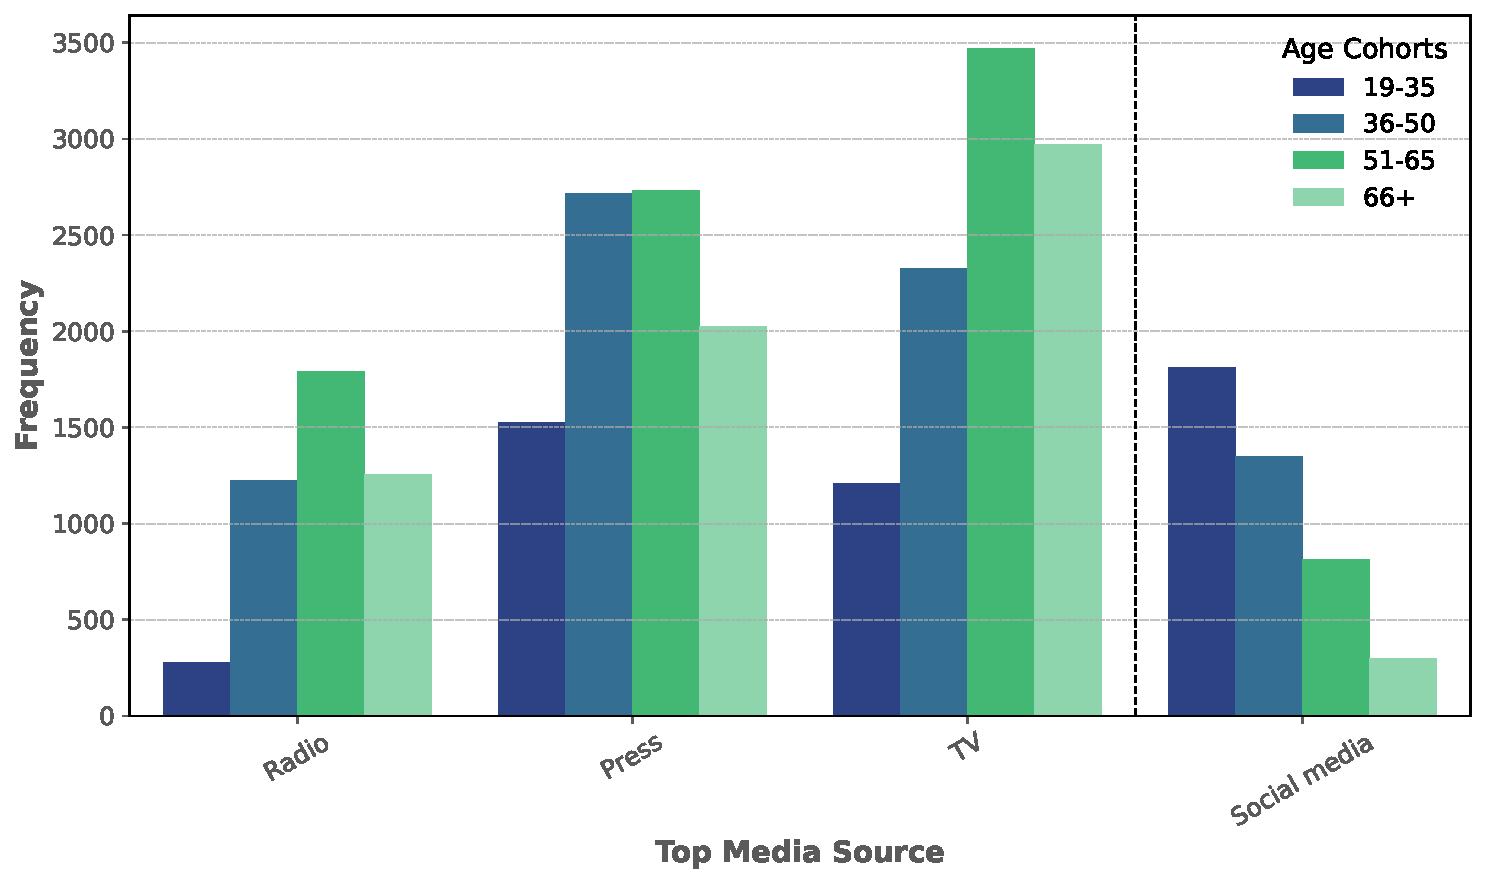
\includegraphics[width=120mm]{figures/age_cohorts}
\caption*{\small Notes: Histogram on the preferred media used for political information in Spain.  
	Source: Barómetro CIS, 2023. }
\label{fig:motivation}
	\end{figure}
	
	

	
	
	
	
	\subsection*{Political Context}
	
	Political power in Spain has historically been dominated by a two-party system, with either the Socialist Party (PSOE) or the Conservative Party (PP) in power. The emergence of the left-wing party Podemos (UP) following the 15M movement marked a significant shift, as the party began to attract a substantial portion of the electorate.\footnote{Relevant for this period of study is the integration of Podemos into the new political party SUMAR. All classification metrics account for this transition, but throughout the text, I refer to UP as either Podemos or SUMAR after its creation.} Of particular interest is the rise of the far-right party VOX, which made notable gains in the regional elections of 2023, raising the possibility of forming a coalition with the Popular Party (PP) in the regional elections held on May 28, 2023. In response, President Pedro Sánchez decided to bring forward the general elections to June 23, 2023 \footnote{ I refer readers to the \href{https://luisignaciomenendez.github.io/media_monitor/index.html}{Spanish Media Monitor} webpage to explore various metrics of coverage across political parties and actors.} 
	
	
	
	

	

	\section{Data and Descriptive Statistics}
	
	\label{section:data}
	
	I built a unique dataset that captures both the demand and supply sides of TV news in the Spanish market. For the demand side, I use minute-by-minute viewership data for the four main channels that offer daily TV news programs: TVE, Antena 3, LaSexta, and Telecinco. On the content side, I build a scraping pipeline that records live the daily news programs and process this information onto text.  This data spans from December 2022 to July 2023 on a daily frequency. 
	
	
	
	\textbf{Audience data }
	
	
	I make use of audimeter, high-frequency audience data provided by Kantar Media.  I  observe the shares of viewers for each channel on a given day and minute. Although I don't have individual data on choices, I do have geographical disaggregation for the 16 Autonomous regions in Spain (also referred to as regions hereinafter), which I will match to survey demographics.\footnote{The Canary Islands and La Rioja are excluded due to different time zones and zero market shares; respectively.}

	
	\textbf{TV Content}
	
	I record daily TV news and use Google Cloud infrastructure to store and process the data with \textit{speech-to-text}. Although visuals play a key role in information transmission, I focus only on text transcripts. A more detailed explanation of the entire downloading pipeline can be seen in Appendix Figure \ref{fig:pipeline}.
	
	
	
	I focus only on the night edition of TV news programs for several reasons. First, it is the so-called "golden time" of the day, attracting the maximum number of viewers on TV. Second, even though channels offer other political programs, the homogeneity of TV news allows me to make very clean comparisons. These programs are broadcasted every day at almost the same time and all share a very similar structure, with a presenter introducing the main stories of the day. The well-known informational motives of these shows ensure that people seek to get informed but do so through the outlet that treats news in their preferred way, either due to some perceived outlet quality or differences in the way content is presented. Third, all TV news are highly fact checked and they remain the most trusted source of information in Spain \footnote{The Digital News Report 2023 reveals notable patterns in public trust towards news media across Europe, with Spain reflecting a stable but modest level of confidence. According to the Digital News Report 2023, the public service broadcaster RTVE and Antena 3 Noticias continue to rank as the most trusted news sources, with trust levels of 53\% and 52\% respectively. laSexta registers a trust increase of 2.7 percentage points over the previous year, reaching approximately 47\%, and Telecinco follows at 39\% \citep{reuters_dnr_2023}.}
	
	
	
	
	\textbf{Agencia EFE}
	
	I obtain all news stories provided in Spanish by one of the largest news agencies in the world, Agencia EFE. Due to access limitations, I receive only the title of each story along with a short summary segment. The sample contains a total of 41K stories for my sample period. 
	
	\textbf{Survey Data}
	
	To understand polarization behavior, I use survey data gathered from the Centro de Investigaciones Sociológicas (CIS). Specifically, I rely on the "intention to vote" question and map it into my binary left-right spectrum. 
	
	\textbf{Weather}
	
	I use meteorological data of daily precipitations per Autonomous Community on the time-span matching the TV news programs (18h-00h) from the Spanish Meteorological Agency (AEMET).
	
	
	
	\subsection{Political Coverage and Elections}
	
	
	
	
	Due to sample restrictions, I divide the time span into two. The \textit{pre-campaign} period starts at the beginning of our data collection in December 2022 and extends to the start of the first publicly announced political campaign on May 13, 2023. The \textit{campaign} period covers both regional and general election campaigns and lasts until the day of the general elections, July 17, 2023.
	
	Figure \ref{fig:coverage} shows the (weekly) average proportion of time devoted to national politics over time; where the \textit{campaign} period corresponds to the shaded time span and vertical dashed lines mark the beginning of the campaign, the regional and the national elections; respectively.  A channel is defined to spend one minute on national politics if the associated text for that minute contains any of the party matches in the dictionaries in table \ref{table:politics}. Pre-campaign, channels spend on average nearly 18\% of their daily time on politics. Naturally, this increases to 30\% in campaign periods. 
	
	\begin{figure}[h!]
		\caption{Proportion of time devoted to politics over time}
		\centering
		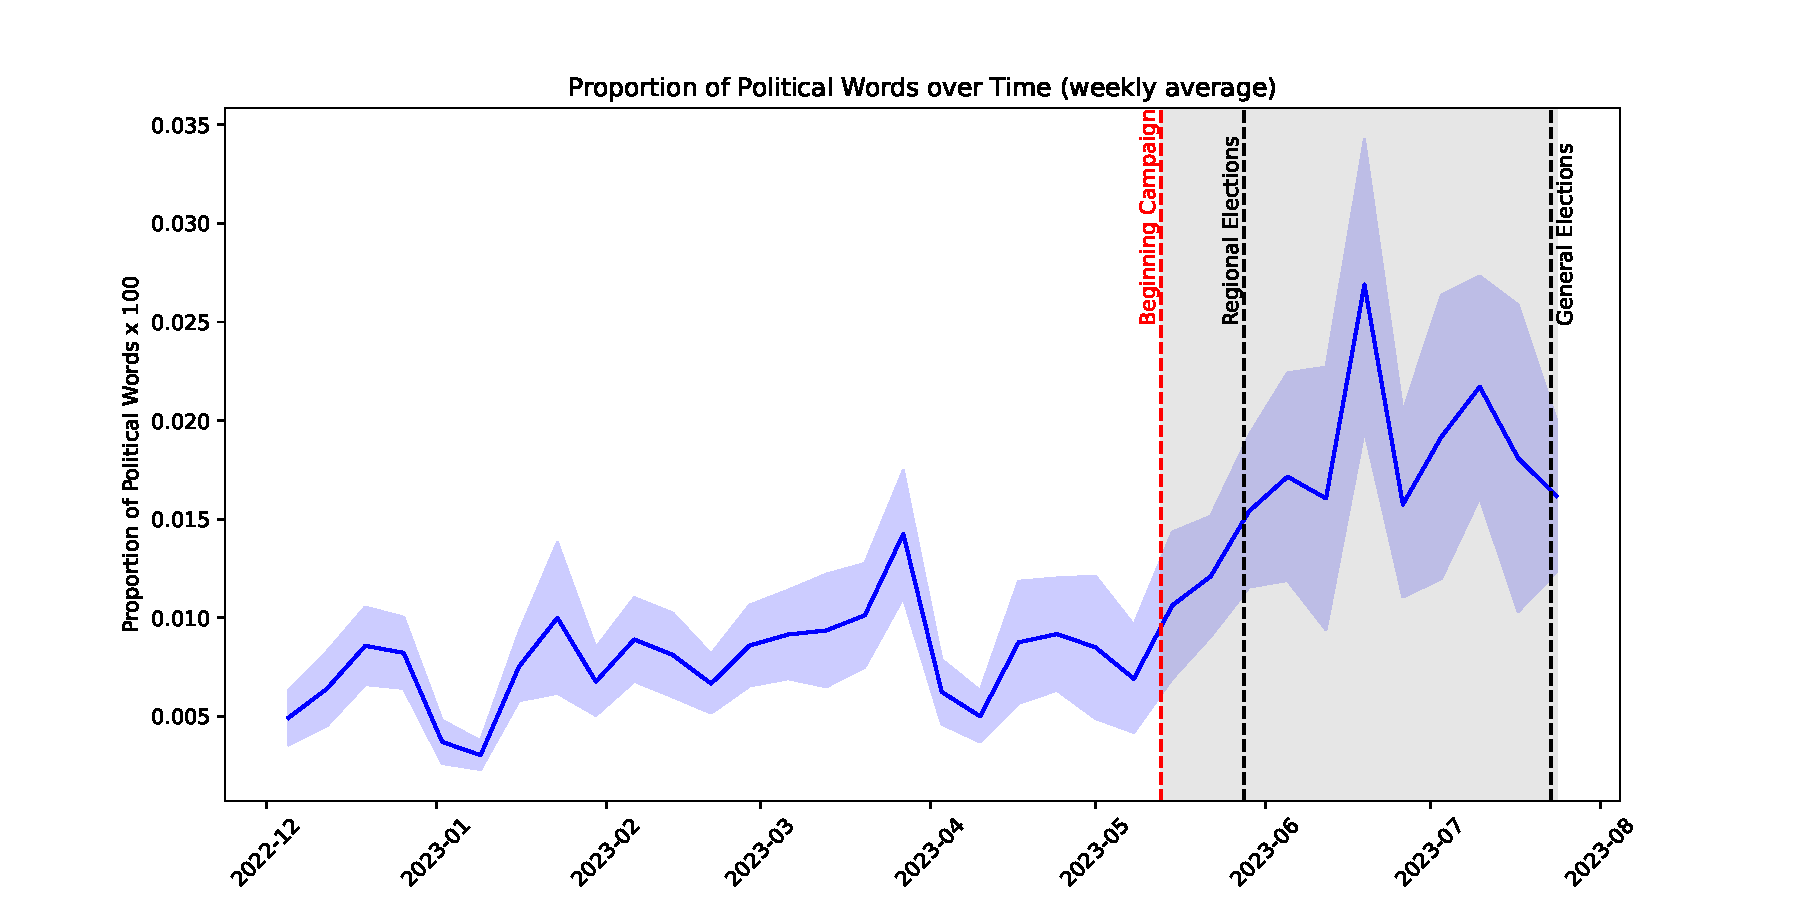
\includegraphics[width=120mm]{figures/political_words2}
		\caption*{\small Notes: Average daily proportion of political terms relative to overall words with shaded standard deviations. Vertical, dashed lines indicate the date of the regional and general elections, respectively. The shaded area represents the "campaign" period considered.}
		\label{fig:coverage}
	\end{figure}
	
	
	
	
	\subsection{ Political Tone}
	
	
	Here I describe the methodology used to classify the political tone of the content broadcasted. I first document the political orientation of the audiences and then use this as intuitive benchmark to validate the content after classification. 
	
	
	\subsection*{Political orientation of the audience }
	
	
	Figure \ref{opinion} shows the correlation between political orientation and preferred channel for acquiring political information, based on survey data from the Centro de Investigaciones Sociológicas (CIS). Right-wing individuals (PP-VOX) tend to watch Antena 3 more, whereas left-leaning individuals are divided between LaSexta and the public channel TVE. We can also observe that the correlation with Telecinco initially appears counterintuitive: it attracts viewers from both extremes of the political spectrum, supporting the hypothesis that third factors, such as entertainment, may influence their choice.
	
	\begin{figure}[h!]
		\centering
		\caption{Correlation between preferred channel and political party}
		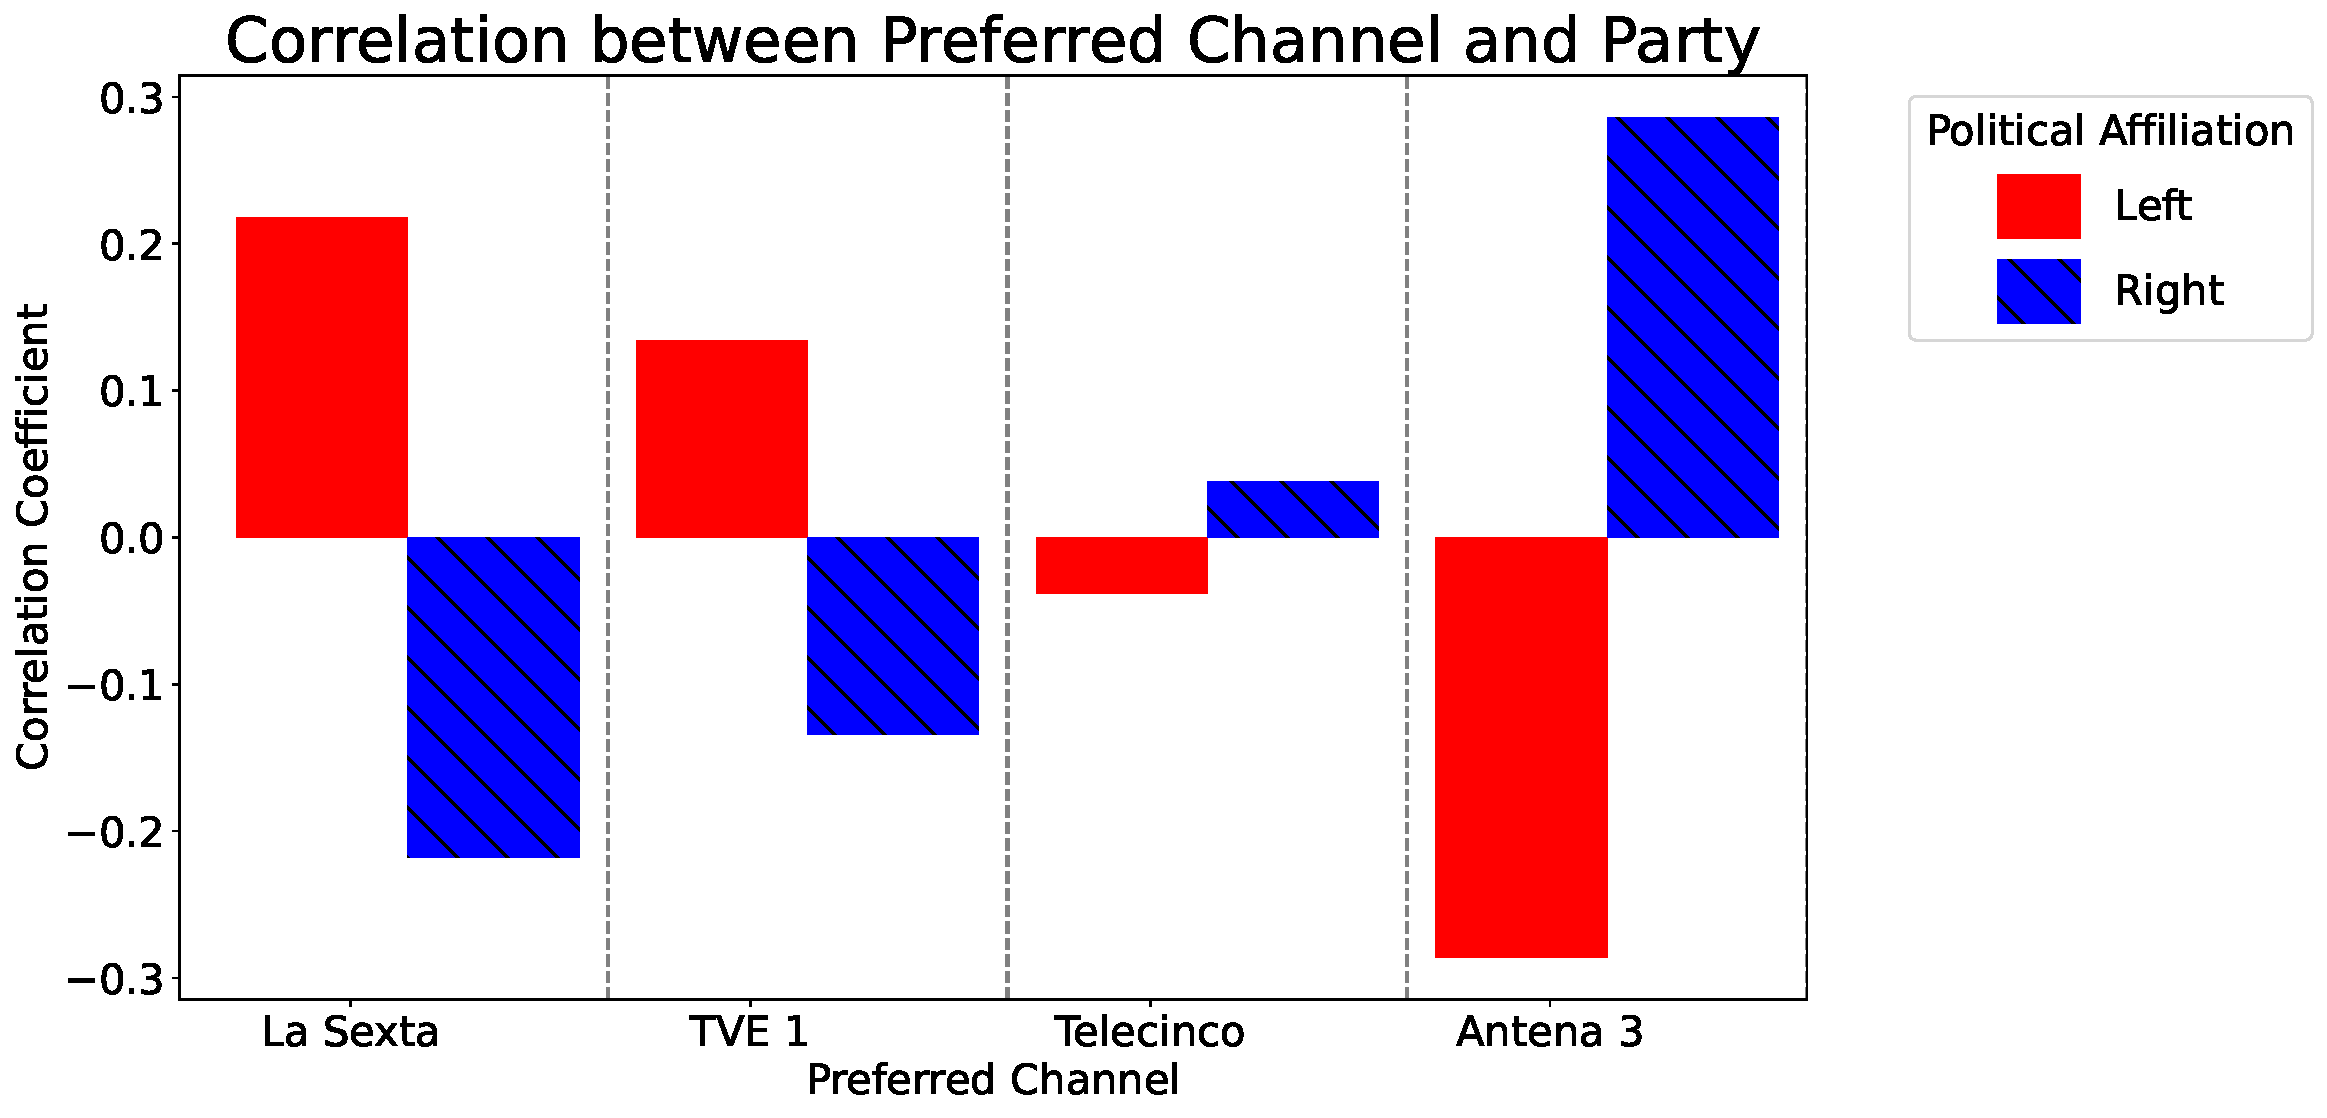
\includegraphics[width=120mm]{figures/corr_party_channel3}
		\caption*{\small Notes:  Bars represent a correlation coefficient between the declared preferred political party (pooling left and right parties) and the most watched channel. The survey ask respondents if they watch TV for political content and what is their preferred channel. Source: Built using data from CIS's Encuesta Pre-electoral 2023 }
		\label{opinion}
	\end{figure}
	
	I also build a density estimate of the audience prefenreces based on the audience shares.	Figure \ref{fig:density} shows the political density in the left right spectrum of each channels' audience using demographics $y$. The left-right position is consistent with the survey correlations shown above and allows me to use these broad preferences as a benchmark from what to expect from the political slant of the outlets. 
	
	
	
	\subsection*{Text Classification}
	
	
	Do channels align with their viewers' demand in the political content they offer? Traditionally, basic text analysis methods, such as measuring mentions or airtime devoted to political actors, have been used to assess plurality and sometimes interpreted as a positive indicator for providing greater publicity. Similarly, sentiment analysis techniques based on semantics cannot reliably discern named entities or context. For this reason, I rely on Large Language Models to classify the stories of the day. The use of LLMs as classifiers has gained popularity in recent years for a variety of context such as classification of political stances \citep{lemens} and has even been found to archive higher precision and accuracy scores for ideological classification when compared to human annotators \citep{tornberg2023}.
	
	
	
	Specifically, I use the latest version of ChatGPT-4, feeding it all our political stories and asking it to classify the tone associated with each political party. Notably, I distinguish between positive and negative tones toward the four political parties considered, and I provide a flexible query that allows the classifier to be neutral if the content is ambiguous. More details about the prompt and classification results can be found on Appendix \ref{sec:chat_gpt}.
	


The challenge is now to map these tone measures accounting for the intensity. I describe below how I combine air-time with tone to build content characteristics. 
	
	
	
	
	\textbf{Building Content Characteristics}
	
	
	In order to create a content description of the daily programs, I consider a set up where each day a channel produces a number of stories $S_{jd}$ indexed by $s$. A story is characterized by a party $ p(s) \in \{L, R, \emptyset\} $, a tone $ \tau(s) \in \{-1, 0, 1\} $ and the number of minutes it spans; $min(s)$. Then the proportion of positive and negative minutes together with the proportion of time devoted to national politics is defined as: 
	
	

		\begin{equation}\label{eq:controls}
		\begin{aligned}
			x_{jd}^{party+}&= \frac{1}{min_{jd}} \sum_{s \in S_{jd}}\bigg(\mathds{1}\{\tau(s)=1\} \times \mathds{1}\{p(s)=party\}\times min(s) \bigg) \quad \forall party \in \{L,R\} \\
			x_{jd}^{party-}&= \frac{1}{min_{jd}} \sum_{s \in S_{jd}}\bigg( \mathds{1}\{\tau(s)=-1\} \times \mathds{1}\{p(s)=party\} \times min(s)\bigg) \quad \forall party \in \{L,R\} \\
			x_{jd}^{political}&=\frac{1}{min_{jd}} \sum_{s \in S_{jd}}\bigg(  \mathds{1}\{p(s)\neq\emptyset\}\times min(s) \bigg)
		\end{aligned}
	\end{equation} 
	
	These variables will constitute the main controls on the empirical application in the next section.  Figure \ref{fig:chat} shows the net average tone relative to total time spent on politics $ \frac{\bar{x}_j^{party+}  - \bar{x}_j^{party+} }{\bar{x}_j^{political}}$ for each party-outlet. This measure acounts both for intensity as it takes into account the minutes that each channel spends on each category and controls for their overall time spent on poliics. Whilst all channels present a negative net tone on the right, there are still significant differences that allow to map them into a different political spectrum. Both La Sexta and the public channel, TVE, offer more pro-left content. Telecinco appears in the middle but still mantains a pro-left stance and Antena 3 is the only one with a more pro-right balance. 	 Both Figures \ref{opinion} and \ref{fig:chat} reinforce the idea that viewers tend to self-select into channels that align with their political preferences, further illustrating the patterns of ideological segregation in media consumption.
	
	
	
	
	
	\begin{figure}[h!]
		\caption{Average sentiment across channels and parties}
		\centering
		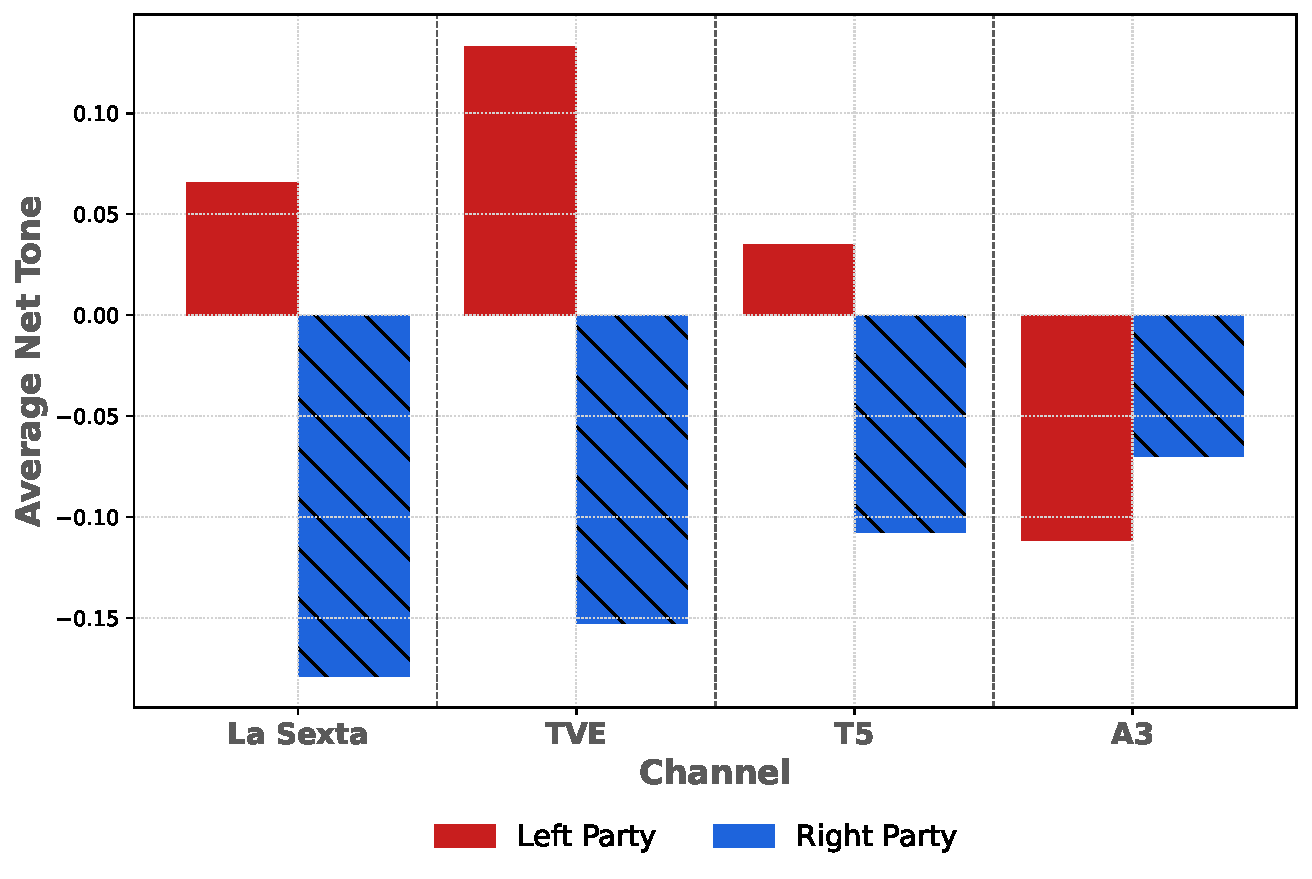
\includegraphics[width=120mm]{figures/chatgpt}
		\caption*{\small Notes: Average tone for each channel-party as classified by Chat GPT 4 from the whole sample period. }
		\label{fig:chat}
	\end{figure}
	
	The results match closely those from declared survey data. 	Figure \ref{fig:channel_ideology_lines} shows the normalized left-right position of the channels based on the survey data shown in \ref{fig:tone2} and the ChatGPT classification. 
	
	
		\begin{figure}[ht]
		\centering
		\caption{Normalized Ideology Scores by Channel}
		% Panel (a): ChatGPT-based
		\begin{minipage}[t]{0.48\textwidth}
			\centering
			\textit{(a) ChatGPT-based Classification}
			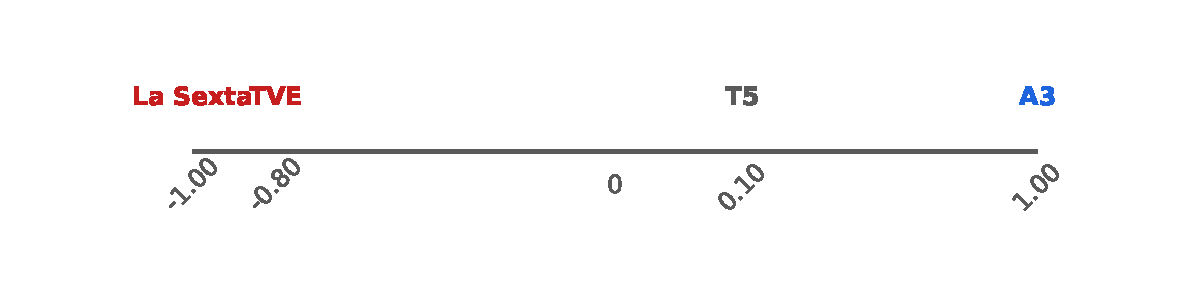
\includegraphics[width=\linewidth]{figures/congress_line_chatgpt}
			
		\end{minipage}
		\hfill
		% Panel (b): CIS-based
		\begin{minipage}[t]{0.48\textwidth}
			\centering
			\textit{(b) CIS-based Classification}
			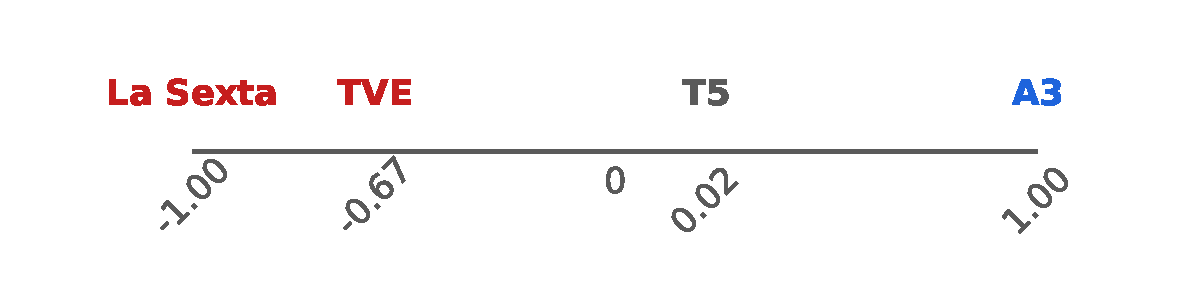
\includegraphics[width=\linewidth]{figures/congress_line_cis}
			
		\end{minipage}
		
		
		\caption*{\small \textit{Notes:} The figure compares normalized left–right audience positions for Spanish television channels. Panel (a) uses ChatGPT-based text classification; panel (b) uses viewer ideology data from CIS surveys. Channels are mapped into the $[-1,1]$ scale using their correlation (tone) and normalizing values into this scale. }
		\label{fig:channel_ideology_lines}
	\end{figure}
	
	
	\textbf{Robustness of  the text classification}
	
	Two main concerns arise with the use of LLMs as text classifiers. First, LLM's have been shown to suffer from potential stochasticity making results unstable when using multiple runs of the same prompt.  Second, one can wonder about performance with other text classification methods.
	
	Due to their inherent stochasticity, repeated queries using the same prompt may yield different classifications. As shown in \citet{llmclassification2024}, this variability can introduce noise in tasks that require high consistency, particularly in content classification. To mitigate this issue, I leverage OpenAI’s ``functions''  tool, which constrains the classifier’s responses to predefined discrete, numerical outputs, reducing potential inconsistencies.  Table \ref{tab:table_stability} presents the mean classification scores from 100 iterations of a random sample of political stories, along with the corresponding standard errors. The relatively small standard errors suggest that despite the model’s stochastic nature, the classification remains stable, in line with the findings of \citet{llmstability2024}, who recommend running multiple iterations when using LLMs as classifiers.
	
	
	The second concern is more fundamental as it challenges the validity of the LLM reasoning as a valid tool for political classification. To address the robustness of its results, I compare the classification results of the LLMs methodologies employed in previous works. I make use of all Spanish congress speeches during my sample period and exploit party labels  to see similarities with the outlet's content \citep{gentzkow2010media}  \citep{laver2003extracting}. The digression in Appendix \ref{sec:sent_stability} explains the methodology in detail. Importantly, figure \ref{fig:congress_line} represents the left-right mapped positions under this method which consistently map the ChatGPT classification in figure \ref{fig:chat} and confirms the power of this approach. 
	
	
	
	\section{Preferences for Politics}\label{section:politics}
	
	\subsection{Political Tone and Electoral Campaign}
	
	The analysis in the previous sections indicates a general distaste for hard news but does not allow us to comment on tolerance for different political parties. In this section, I explore whether there has been asymmetric distaste for different political parties in response to the campaign period. We begin by detailing how channels have varied their tone toward the parties during this period \citep{independent2023vox}.
	
	We decompose relative tone before and during campaign periods in Figure \ref{fig:tone2}, relative to the number of minutes covered on national politics. The left-leaning channel, LaSexta, significantly reinforced its left position by increasing the positive tone on left-wing parties and decreasing it on both right-wing parties. All other outlets opted for a moderating effect, reducing their mean relative tone.
	
	
	
	
	
	\section{Market set up}\label{section:market}
	
	The TV market set up differs from the classical demand estimation problem as there is absence of prices and channels differentiate themselves varying product characteristics. I estimate demand using a mixed logit model \citep{berry1994estimating} \footnote{The model is estimated under the \textit{pyblp} package \citep{conlon2020best}.}.
	
	
	
	An individual $ i $  a region $r$ chooses an outlet $ j \in \mathcal{J}\equiv \{La6,TVE,T5,A3,\emptyset\}$ to watch at the beginning of day $d$ based on the following indirect utility : 
	
	
	\begin{equation}\label{eq:utility}
		\begin{aligned}
			& U_{ijrd}= \underbrace{\sum_k x_{jd-1}^k\alpha^k+w_{rd}\gamma  +  \xi_{jrd}}_{\delta_{jrd}}  + \underbrace{  \sum_k x_{jd-1}^k \Big( \sigma^k \nu_{ird}^k  + \pi^ky_{ir} \Big)}_{\mu_{ijrd}}+\epsilon_{ijrd} 
		\end{aligned}
	\end{equation} 
	
	where $ x_{jd}^k $ represents the $ k \in \{R+,R-,L+,L-,political\}$ characteristic on channel $ j $ and day $ d$ as defined in \ref{eq:controls}. $ \sigma^k $ is a shift on characteristic $ k $ mean preferences according to unobserved preferences $ \nu_{ird}^k \sim N(0,1)$.  The  characteristic $w_t$ measures the precipitation level on a given day-region. I also introduce as demographics, $ y_{ir} $ that represent whether individual $i$ is right wing or not according to survey data. Thus the parameters $\pi^k$  capture polarization behavior where more right-wing viewers have asymmetric tastes for content on their own and the opposed party tone. 
	
	
	
	I decompose the unobserved characteristics into $\xi_{jrd}= \xi_j + \xi_{dow} + \Delta \xi_{jrd}$, where I include product dummies that account for unobserved quality factors and day of the week dummies to control for  seasonality. 
	
	The outside option is modeled in terms of \textit{potential} audience. Formally, the observed share of people consuming a channel  is $ s_{jrd}\equiv \frac{q_{jrd}}{L_{r}}$where $ q_{jrd} $ is the (initial) total number of viewers watching channel $ j $ and  $ L_{r} $ is the potential of viewers having access to TV on region $ r$; defined by Kantar media as the population that has access to television in a given region. Importantly, I fit the model using data from the first 5 minutes of the day, where viewers have not been exposed to the daily content yet. This timing will become important for the supply identification later on. 
	
	Market shares are just the integral over the individual choice indicators:  
	
	
	\begin{equation}\label{eq:shares}
	\begin{aligned}
		& s_{jrd} = \int d_{ijrd}(\bm{\delta_{rd}},\bm{\mu_{ird}})d\bm{\mu}_{ird}d\bm{\epsilon}_{ird}
	\end{aligned} 
\end{equation} 
	
	where $d_{ijrd}$ equals $1$ if $U_{ijrd}>U_{ikrd} \quad \forall j\neq k$ and $0$ otherwise. Survey weights are included in the integration. 

	
	\subsection{Content endogeneity and News Shocks} \label{section:endogeneity}
	
	
	Content characteristics are an equilibrium outcome of the differentiation game therefore creating endogeneity problems due to simultaneity bias.  Figure \ref{fig:diagram} illustrates the trafe-offs in the model. Viewers make expectations about the utility for each choice. This depends on exogenous factors such as weather, individual attrbitues (i.e ideology) and shcoks that are unobserved to the econometrician; $ \xi$.  On the supply side, channels make their content decisions for the next day forecasting their audience tastes and the shocks that the might have the next day. Editors tweak today’s rundown knowing which stories will make viewers lean in tomorrow. The red dashed arrow indicates thus the endogeneity concern $\E(\mathbf{x}_{jrd-1}\xi_{jrd})\neq \mathbf{0} $.
	
	
	\begin{figure}
				\caption{Trade-offs in the model}
				\label{fig:diagram}
			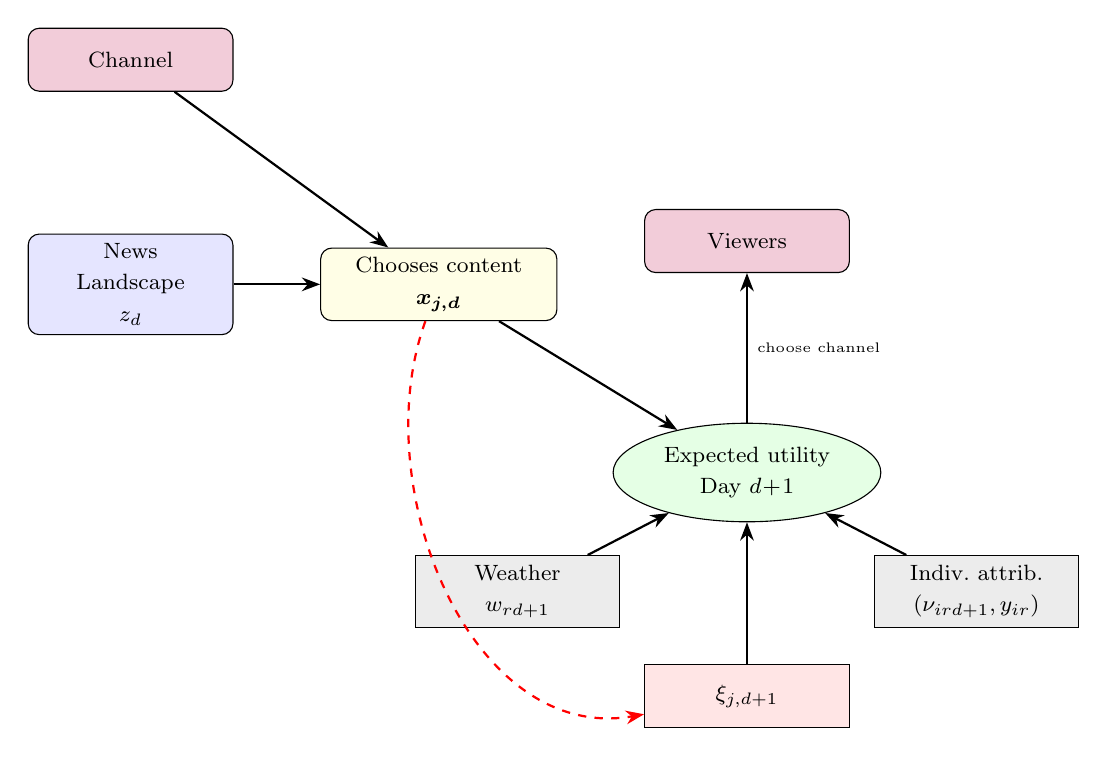
\begin{tikzpicture}[
			inst/.style   ={rectangle, draw, fill=blue!10,  rounded corners, align=center,
				minimum width=2.6cm, minimum height=0.8cm},
			decision/.style={rectangle, draw, fill=yellow!10, rounded corners, align=center,
				minimum width=3.0cm, minimum height=0.9cm},
			util/.style   ={ellipse,   draw, fill=green!10,  align=center,
				minimum width=3.4cm, minimum height=1.0cm},
			shock/.style  ={rectangle, draw, fill=red!10,   align=center,
				minimum width=2.6cm, minimum height=0.8cm},
			exo/.style    ={rectangle, draw, fill=gray!15,  align=center,
				minimum width=2.6cm, minimum height=0.8cm},
			actor/.style  ={rectangle, draw, fill=purple!20, rounded corners, align=center,
				minimum width=2.6cm, minimum height=0.8cm},
			flow/.style   ={-Stealth, thick},
			feed/.style   ={dashed,-Stealth, thick, red},
			node distance = 1.8cm and 1.1cm,
			font=\footnotesize
			]
			% -------- DAY d (supply) ---------
			\node[inst]                    (news)   {News\\Landscape\\$z_{d}$};
			\node[actor, above=of news]    (channel) {Channel};
			
			\node[decision, right=of news] (x)      {Chooses content\\$\bm{x_{j,d}}$};
			
			% -------- DAY d+1 (demand) ------
			\node[actor, right=of x, yshift=0.55cm] (viewer) {Viewers};
			
			\node[util,  below=of viewer, yshift=-0.1cm] (util)
			{Expected utility\\Day $d\!+\!1$};
			\node[shock, below=of util]     (xi)     {$\xi_{j,d+1}$};
			\node[exo,   below left=0.6cm and 0.4cm of util]
			(weather){Weather\\$w_{rd+1}$};
			\node[exo,   below right=0.6cm and 0.4cm of util]
			(prefs)  {Indiv.\ attrib.\\$(\nu_{ird+1},y_{ir})$};
			
			% ---------- flows ---------------
			\draw[flow] (channel) -- (x);
			\draw[flow] (news)    -- (x);
			\draw[flow] (x)       -- (util);
			\draw[flow] (prefs)   -- (util);
			\draw[flow] (weather) -- (util);
			\draw[flow] (xi)      -- (util);
			\draw[flow] (util)    -- (viewer) node[midway,right,font=\tiny]{choose channel};
			
			% ------ anticipation feedback ---
			\draw[feed] (x) to[out=-110,in=190] node[midway,below,font=\tiny]
			{} (xi);
			\end{tikzpicture}

	\end{figure}
	
	
	
	

	
	To address this endogeneity concern, I instrument for each of the $k$ endogenous product characteristics using supply shocks. I proxy the daily news landscape by using all available stories ( $N\approx41\text{K}$) from Spain provided by Agencia EFE, one of the largest communication agencies in the world. Importantly, unlike traditional media such as newspapers, television stations rely heavily on third-party news aggregators to purchase stories, images, and related content.	All the channels considered in this study collaborate with Agencia EFE, thereby minimizing concerns about the agency having a specific political bias or being uninformed\footnote{See collaborations for \href{https://www.telecinco.es/autores/agencia-efe/}{Mediaset}, \href{https://cadenaser.com/nacional/2024/09/22/el-teletexto-una-herramienta-olvidada-que-aun-perdura-en-nuestras-televisiones-cadena-ser/}{Atresmedia}, and \href{https://www.rtve.es/rtve/20130301/rtve-agencia-efe-firman-convenio-colaboracion/611440.shtml}{RTVE}.}.
	
	
	Analogous to the content covariates in \ref{eq:controls}, I control for the political composition of the news landscape using the relative number of stories available for each of the $K$ characteristics: 
	
	
	\begin{equation}\label{eq:first_stage}
		\begin{aligned}
			z_d^{party+}&= \frac{1}{|S_d|} \sum_{s \in S_d}\bigg(\mathds{1}\{\tau(s)=1\} \times \mathds{1}\{p(s)=party\} \bigg)\quad &\forall party \in \{L,R\}\\
			z_d^{party-}&= \frac{1}{|S_d|}\sum_{s \in S_d}\bigg( \mathds{1}\{\tau(s)=-1\} \times \mathds{1}\{p(s)=party\} \bigg) \quad &\forall party \in \{L,R\}\\
			z_d^{political}&=\frac{1}{|S_d|} \sum_{s \in S_d}\bigg(  \mathds{1}\{p(s)\neq\emptyset\} \bigg)
		\end{aligned}
	\end{equation} 
	
	
where I slightly abuse notation and take the relative with respect to the total number of stories in a given day produced by Agencia EFE, $S_d$, and tone of the stories is computed under the same ChatGPT specification and query as in the TV data. 

Importantly for the specification, I assume that channels suffer short run shocks that impede them to place their content at their optimal long-run equilibrium. As an illustration of how this mechanism works in practice, consider the average tone results from \ref{fig:chat}.  
    Channel would like to stick to their ideal positions (i.e those shown in \ref{fig:channel_ideology_lines}) but their production of stories depends on news availability. On days where the news landscape contains more stories on a particular party-tone combination, outlets are less or more constrained depending on whether this allows them to get closer to their ideal points. 

	\begin{comment}
	\begin{figure}
		\centering
		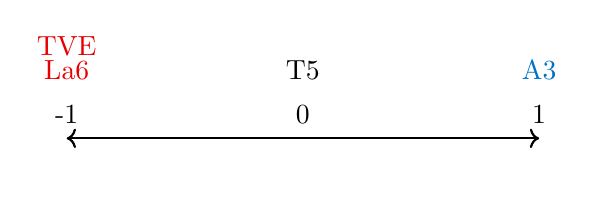
\begin{tikzpicture}
			% Draw the line with arrows
			\draw[<->, thick] (-3,0) -- (3,0);
			
			% Add the numerical labels for -1, 0, and 1
			\node at (-3,0.3) {-1};
			\node at (0,0.3) {0};
			\node at (3,0.3) {1};
			
			% Define positions for the channels
			\node (TVE) at (-3, 0) {};
			\node (La6) at (-3, 0) {};
			\node (T5) at (0, 0) {};
			\node (A3) at (3, 0) {};
			
			% Draw the channel names above the line
			\node[above=0.5cm of TVE] {\textcolor{PSOEred}{La6}};
			\node[above=0.8cm of TVE] {\textcolor{PSOEred}{TVE}};
			\node[above=0.5cm of T5] {T5};
			\node[above=0.5cm of A3] {\textcolor{PPblue}{A3}};
			\node[below=0.2cm of T5] {};
			
		\end{tikzpicture}
		\caption{Illustration of the channel's equilibrium position in the political spectrum according to their average reported tone on left and right channels. }
		\label{fig:game}
	\end{figure}
	\end{comment}
	




	
	
	
Tables \ref{tab:neg_left_channels} and \ref{tab:neg_right_channels} illustrate this mechanism by displaying the stories from the most negative day for the left- and right-wing parties, respectively. The most unfavorable day for left-wing parties in the sample is February 27, 2023. On this day, a technical failure in the "ley solo sí es sí" law, promoted by the left-wing party Unidas Podemos, resulted in reduced sentences for convicted rapists. Additionally, a motion of no confidence was submitted against the Socialist Prime Minister Pedro Sánchez, and the corruption scandal known as "Caso Mediador" was affecting the government. The distribution of airtime dedicated to negative left-wing content varies across channels: A3 allocates nearly 19\%, followed by TVE and Telecinco with 4\% each, and La Sexta with only 2\%.

Conversely, the day with the highest volume of negative coverage for right-wing parties was May 17, 2023. On this day, several events contributed to negative media coverage: a scandal involving the brother of Isabel Díaz Ayuso, the president of Madrid’s regional government (PP), the rejection of a right-wing party’s motion in the Senate, and reports of police abuse against protesters participating in a march against the extreme right party VOX. The pattern observed on February 27 is reversed in this case: La Sexta dedicates nearly 15\% of its airtime to negative right-wing content, followed by TVE and Telecinco, while A3 allocates only 4\%.
	
	
	
	In order to show the previous mechanism outlined in these examples in practice, I run separate reduced form regression for each party-tone combination of the form: 
	
	

	
	\begin{equation}\label{eq:pred_pos}
	\begin{aligned}
x^{party+}_{jd}=& \sum_{party \in \{L,R\}} \sum_{j' \in \mathcal{J} }  \left(d(j')_j \times z^{party+} _d      \right) \beta_{j}^{(party,+ )}  + \\
		+ &   \sum_{party \in \{L,R\}} \sum_{j' \in \mathcal{J} }   \left(d(j')_j \times z^{party-} _d      \right) \beta_{j}^{(party,- )} +    \sum_{j' \in \mathcal{J} }   \left(d(j')_j \times z^{political}_d      \right) \delta_{j} +\epsilon_{jd}
	\end{aligned}	
\end{equation} 



\begin{equation}\label{eq:pred_neg}
	\begin{aligned}
	x^{party-}_{jd}=& \sum_{party \in \{L,R\}} \sum_{j' \in \mathcal{J} }  \left(d(j')_j \times z^{party+} _d      \right) \phi_{j}^{(party,+ )}  + \\
		+ &   \sum_{party \in \{L,R\}} \sum_{j' \in \mathcal{J} }   \left(d(j')_j \times z^{party-} _d      \right) \phi_{j}^{(party,- )} +    \sum_{j' \in \mathcal{J} }   \left(d(j')_j \times z^{political}_d      \right) \rho_{j} +\epsilon_{jd}
	\end{aligned}
\end{equation} 
	
	
	A positive $ \beta_{j}^{R,+} $ coefficient indicates that given an extra positive story about the right wing party is available, outlet $ j $ increases the number of positive stories about that party by $  \beta_{j}^{R,+}  $, ceteris paribus. 
	
	\begin{comment}
Figure \ref{fig:prediction2} show the predicted news composition balance ( $\hat{x}^{party+} - \hat{x}^{party-}$ ) for simulated favorable and unfavorable days for the left and right based on news availability $ \mathbf{z}$. 

	
The top left panel shows that on days highly unfavorable for the left, it is the right channel that presents a more negative scenario for that party. Conversely, days with dominant positive left stories (bottom left graph) only look favorable from the left channels perspective. This illustrates that, even though the shock of news is common to all channels, their intrinsic ideology makes them asymmetrically constrained in their news production and can be used as an instrument. The exclusion restriction implies that audience does not ex-ante react to different composition of the day. For instance, if viewers knew that a scandal happened and they switched to their preferred outlet to watch it, that would violate the identification assumption. Although this cannot be tested directly, I show that using the minute 0 audience (i.e before any content has been shown already), I do not find asymmetric audience gains across outlets based on the composition of the day. Results are shown in appendix table \ref{table:check_exogeneity}.
	
	\end{comment}
	
	
	Figure \ref{fig:fwl} shows the added variable plots from equations  \ref{eq:pred_neg} and \ref{eq:pred_pos} for each channel.  Rows correspond to the dependent variable $x_{jd}^{party+}$  or $x_{jd}^{party-}$  and columns to  $z_{d}^{party+}$  and  $z_{d}^{party-}$, respectively.  
	
	
	 An increase of 1pp. of negative left stories is associated with a 0.49pp increase in relative time devoted to negative left wing content in the right wing channel versus a 0.27 for the left channels, ceteris paribus. The reversed situation happens when we look at positive left content. Left wing channels now produce a higher content compared to the right wing channel. These patterns alltogether illustrate the effectiveness of the shocks in practice: Outlets increase production of a particular party-tone content whenever this allows them to stay closer to their long run equilibrium.
	
	
	
	
	\begin{comment}
	\begin{figure}[h!]
		\centering
		\figuretitle{  }
		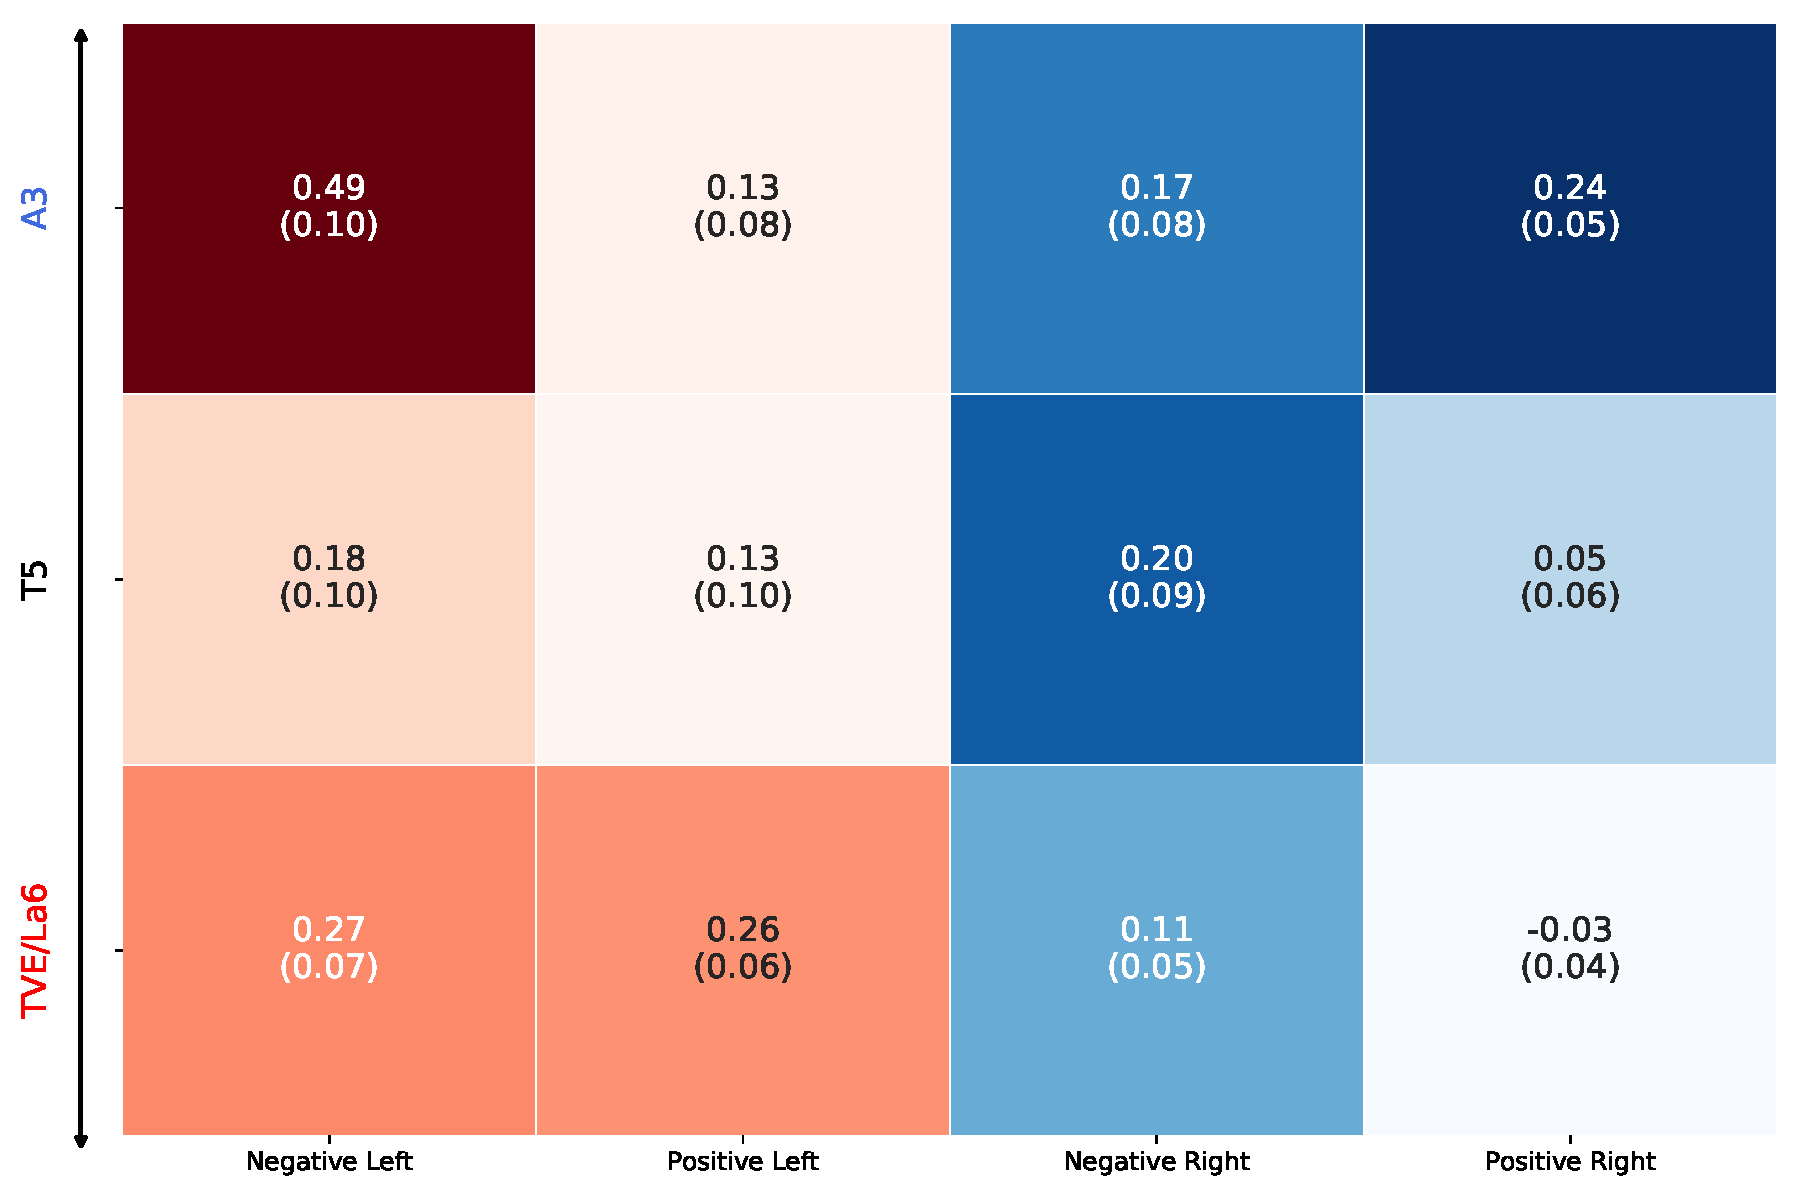
\includegraphics[width=120mm]{figures/heatmap_iv}
		\caption{The heatmap shows the estimated coefficients with standard errors from equations \ref{eq:pred_neg} and \ref{eq:pred_pos}. Rows correspond to the dependent variable $x_{jt}^{party+}$  or $x_{jt}^{party-}$  and values correspond to the coefficient that matches the same party-tone combination, i.e   $\hat{\beta}_j^{(party,+)}, \hat{\phi}_j^{(party,-)}$, respectively. Channels are pooled into left (TVE and La6), middle (T5) and right (A3) for visualization purposes.  }
		\label{fig:heatmap}
	\end{figure}
	\end{comment}
	
	
		\begin{figure}[h!]
		\centering
\caption{Added variable plots for production of political content}
		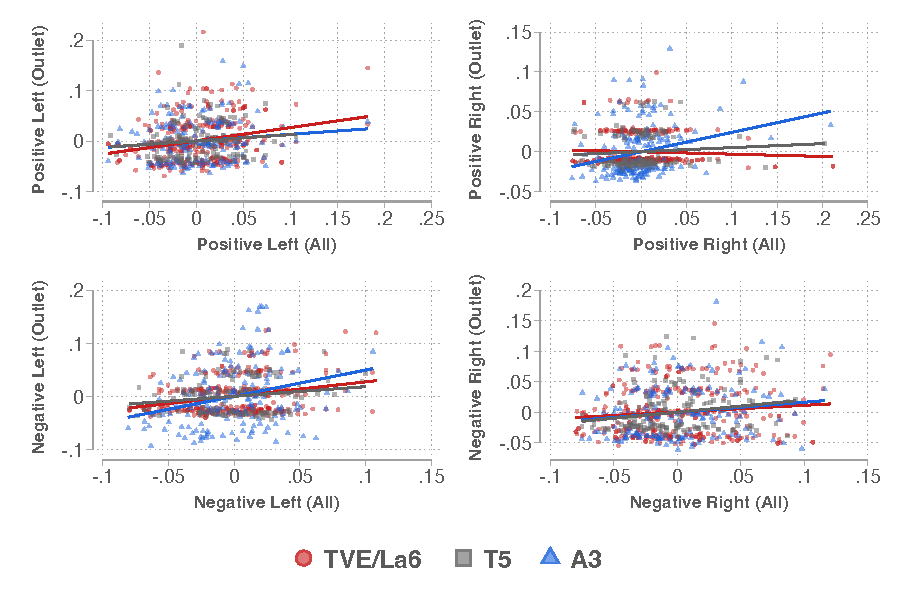
\includegraphics[width=160mm]{figures/fwl_plots}
		\caption*{\small Notes: The figure shows the added variable plots from the estimation of equations   \ref{eq:pred_neg} and \ref{eq:pred_pos}. The x axis represents $(z_d^{party,+},z_d^{party,-}) $ and the y axis the corresponding  $(x_{jd}^{party,+},x_{jd}^{party,-}) $   . Channels are pooled into left (TVE and La6), middle (T5) and right (A3) for visualization purposes.  }
		\label{fig:fwl}
	\end{figure}
	
	
	
	
	\begin{table}[H]
		\centering
	
		\label{tab:tests}
		\caption{F and t-tests for Regression Coefficients}
		\begin{tabular}{lcccc}
			\hline
			Characteristic & F-test  & F-test p-value & T-test  & T-test p-value \\
			\hline
			$ {L-}$& 2.69 & 0.0686 & 3.51  & 0.0613 \\
			$ {L+}$ & 1.31 & 0.2711 & 1.87  & 0.1715 \\
			$ {R-}$ & 0.42 & 0.6594 & 0.34 & 0.5592 \\
$ {R+}$ & 8.78 & 0.0002 & 17.55  & 0.0000 \\
			\hline
		\end{tabular}
			\caption*{\small Notes: Summary of F- and T-test results for equality of news variable coefficients across channels. The F-test evaluates overall equality across channels, while the T-test compares the coefficient of the main independent variable between A3 and TVE/La6.}
	\end{table}
	
	
	
	
\begin{comment}
	
	\begin{figure}[h!] 			
		\centering
		\begin{minipage}[b]{0.5\linewidth}
			\centering
						\caption*{Unfavorable day Left}
			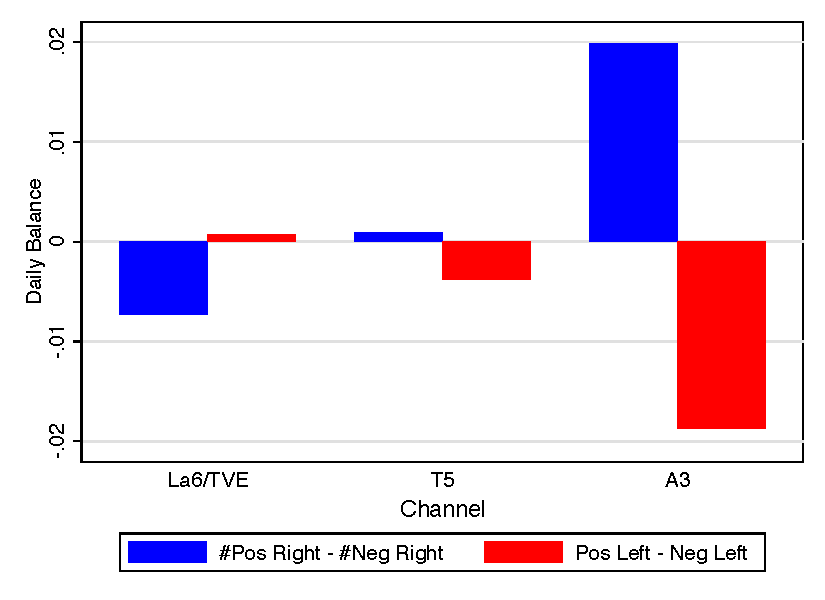
\includegraphics[width=.9\linewidth]{figures/predicted_bad_left} 

		\end{minipage}%%
		\begin{minipage}[b]{0.5\linewidth}
			\centering
						\caption*{Unfavorable day Right}
			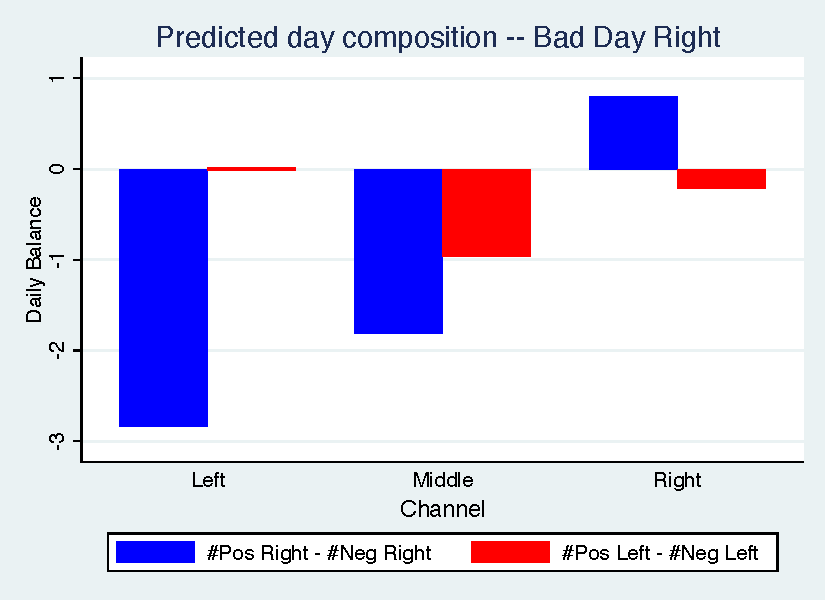
\includegraphics[width=.9\linewidth]{figures/predicted_bad_right} 

		\end{minipage} 
		\\
		\begin{minipage}[b]{0.5\linewidth}
			\centering
						\caption*{Favorable day Left}
			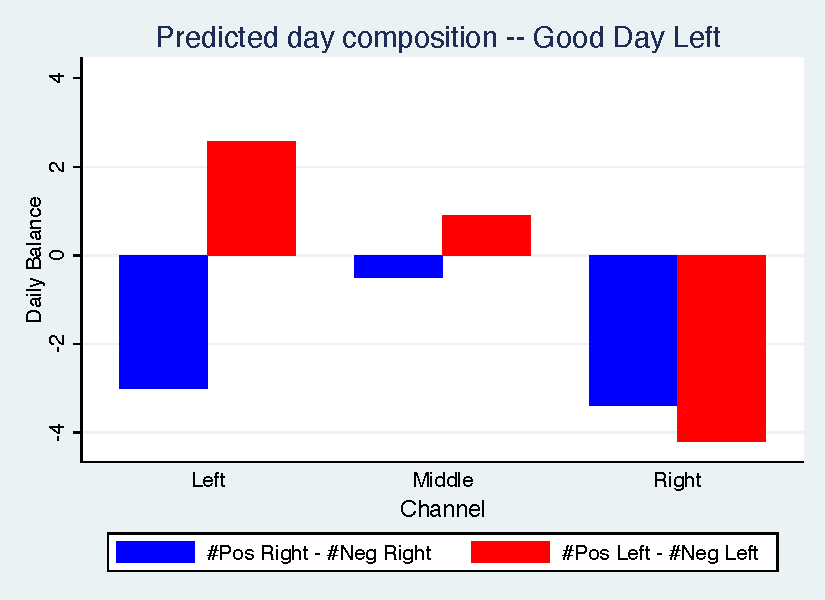
\includegraphics[width=.9\linewidth]{figures/predicted_good_left} 

		\end{minipage}%%
		\begin{minipage}[b]{0.5\linewidth}
			\centering
						\caption*{Favorable day Right}
			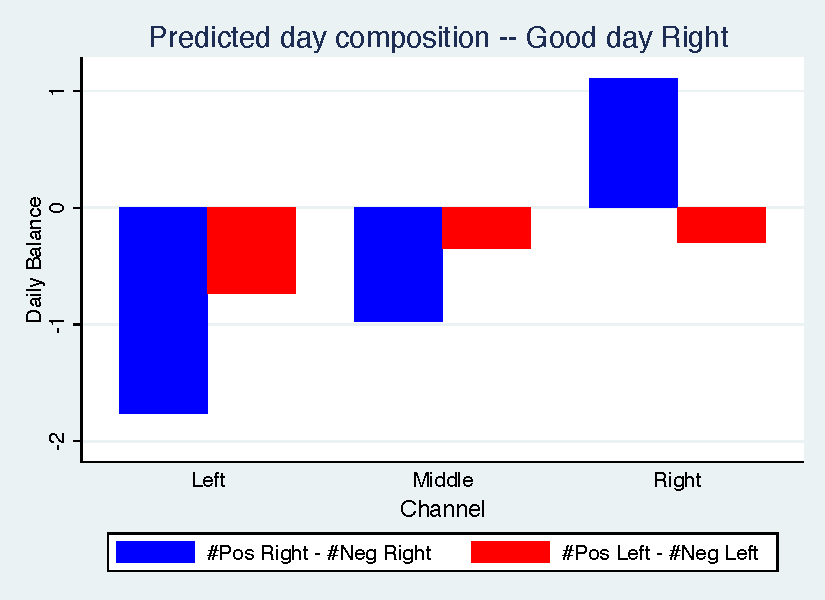
\includegraphics[width=.9\linewidth]{figures/predicted_good_right} 

		\end{minipage}  
			\caption{Predicted number of positive minus negative minutes for each outlet and party. The top left (right) plots show days where 4 negative stories for the left(right) party are available and 1 stories of the other type for the rest. The bottom graphs show the analogous scenario with positive stories. 
			The horizontal axis represents the channel classified by its intrinsic ideology into left (La6 and TVE), Middle(Telecinco) and Right (Antena3).  } 
		
		\label{fig:prediction2} 
	\end{figure}
	\end{comment}
	
	
	
	

Based on the previous discussion, I use $\left(z_d^{party+},z_d^{party+}, z_d^{political}\right)_{party \in \{L,R\}}$	as instruments for the linear characteristics. For the $ K $ non linear coefficients that represent the variance of the individual heterogeneity I follow \cite{gandhi2019measuring} and target predicted product differentiation instruments of the form $ \left(\hat{x}_{jd}^k- \sum_{l \neq j} \hat{x}_{ld}^k\right)^2 $, where $ \hat{x}_{jd}^k $ is the predicted $ k $th characteristic from the first stage of the instrumental variable regression \ref{eq:first_stage}. To target the demographic parameters, I interact the mean proportion of right votes with those instruments: $ \bar{y}_r\hat{x}_{jd}^k $.
	

	
	
	\section{Results}
	
	\label{section:results}
	
	
	I present results of the BLP estimation for the pre-campaign and campaign periods in table   \ref{tab:results_blp}. I show the preferred specification under outlet and day of the week fixed effects with standard errors clustered at the region level. 
	
	The pre-campaign period estimation shows a significant, positive average taste for negative stories on the right party with significance dispersion ($\sigma^{\text{R-}}$) in the population. Importantly, this dispersion is not explained by ideology heterogeneity ($\pi$ coefficients).
	
	
	
	The campaign period estimates showed at the bottom of the table show a somewhat different set up. There is a significant positive taste for positive stories on the left and negative stories on the right parties. This fact, together with the negative taste on positive right and negative left content would indicate an average preference towards the left leaning parties. The coefficients with the interaction with ideology further indicate a result in line with a polarization behavior: more right wing audiences demand content that is more favorable towards their own party and more negative towards the opposition. The fact that this behavior is exhibited only during the political campaign period and not before links to several results on the political information acquisition.  
	
	The taste for national politics overall is negative with right wing viewers having a higher demand for it. 
	
	
	
	\begin{table}[ht]
					\caption{BLP Estimation Results with Standard Errors}
					\label{tab:results_blp}
		\centering
		\begin{threeparttable}
			\begin{tabular}{lccc}
				\hline
				\textbf{Coefficient} & \textbf{Parameter} & \textbf{Estimate} & \textbf{Std. Error} \\
				\hline
				\multicolumn{4}{c}{Pre-campaign} \\
				\hline
				\hline
				Positive Left & $\beta^{L+}$ & -16.90 & (11.73) \\
				Positive Right & $\beta^{R+}$ & -25.53 & (31.03) \\
				Negative Left & $\beta^{L-}$ & 28.29 & (25.89) \\
				Negative Right & $\beta^{R-}$ & 56.44** & (28.45) \\
				Political & $\beta^{political}$ & 11.49*** & (4.28) \\
				Weather & $\gamma$ & 0.00 & (0.03) \\
				\hline
				Positive Left & $\sigma^{L+}$ & 0.44 & (296.90) \\
				Positive Right & $\sigma^{R+}$ & 0.68 & (715.26) \\
				Negative Left & $\sigma^{L-}$ & 12.64 & (8.68) \\
				Negative Right & $\sigma^{R-}$ & 21.99 & (13.83) \\
				Political & $\sigma^{political}$ & 0.00 & (46.79) \\
				\hline
				Right-Wing $\times$  Positive Left & $\pi^{L+}$ & 46.26 & (48.70) \\
				Right-Wing $\times$  Positive Right & $\pi^{R+}$ & 77.81 & (95.92) \\
				Right-Wing $\times$  Negative Left & $\pi^{L-}$ & -70.09 & (57.97) \\
				Right-Wing $\times$  Negative Right & $\pi^{R-}$ & -103.71 & (97.76) \\
				Right-Wing $\times$  Political & $\pi^{political}$ & -25.17** & (12.59) \\
				\hline
				\hline
				\multicolumn{4}{c}{Campaign} \\
				\hline
				\hline
				Positive Left & $\beta^{L+}$ & 134.16** & (65.57) \\
				Positive Right & $\beta^{R+}$ & -129.79*** & (48.43) \\
				Negative Left & $\beta^{L-}$ & -104.84** & (41.32) \\
				Negative Right & $\beta^{R-}$ & 92.62** & (41.63) \\
				Political & $\beta^{political}$ & -6.43** & (3.26) \\
				Weather & $\gamma$ & 0.00 & (0.01) \\
				\hline
				Positive Left & $\sigma^{L+}$ & 0.00 & (320.36) \\
				Positive Right & $\sigma^{R+}$ & 19.25* & (10.89) \\
				Negative Left & $\sigma^{L-}$ & 0.00 & (134.33) \\
				Negative Right & $\sigma^{R-}$ & 0.02 & (73.18) \\
				Political & $\sigma^{political}$ & 0.00 & (19.55) \\
				\hline
				Right-Wing $\times$  Positive Left & $\pi^{L+}$ & -421.99** & (176.15) \\
				Right-Wing $\times$  Positive Right & $\pi^{R+}$ & 334.94*** & (127.41) \\
				Right-Wing $\times$  Negative Left & $\pi^{L-}$ & 288.65** & (116.22) \\
				Right-Wing $\times$  Negative Right & $\pi^{R-}$ & -280.33*** & (104.44) \\
				Right-Wing $\times$  Political & $\pi^{political}$ & 19.34** & (8.93) \\
				\hline
				\hline
			\end{tabular}

			\begin{tablenotes}
				\small
				\item \footnotesize{The table shows the results of the BLP estimation of model \ref{eq:utility}. The estimations are divided into the pre-campaign and campaign period. Both day-of-the-week and outlet fixed effects are included. Standard errors are clustered at the region level. The total number of observations are $N_{campaign}=2307$ and  $N_{pre\_campaign}=6604$.}
			\end{tablenotes}
		\end{threeparttable}
	\end{table}
	
	
	
	
	
	
	
	\begin{comment}
	
	\begin{table}[ht]
		\centering
		\begin{threeparttable}
			\begin{tabular}{lccc}
				\hline
				\textbf{Coefficient} & \textbf{Parameter} & \textbf{Estimate} & \textbf{Std. Error} \\
				\hline
				\hline
				\multicolumn{4}{c}{{Pre-campaign}} \\
				\hline
				\hline
				Positive Left & $\sigma^{L+}$ & 7.04 & (21.28) \\
				Positive Right & $\sigma^{R+}$ & 23.82 & (20.06) \\
				Negative Left & $\sigma^{L-}$ & 3.85 & (11.56) \\
				Negative Right & $\sigma^{R-}$ & 25.42*** & (5.01) \\
				Political & $\sigma^{\text{political}}$ & 3.47 & (7.58) \\
				\hline
				Right-Wing $\times$ Positive Left & $\pi^{L+}$ & 21.75 & (16.78) \\
				Right-Wing $\times$ Positive Right & $\pi^{R+}$ & 35.74 & (43.73) \\
				Right-Wing $\times$ Negative Left & $\pi^{L-}$ & -48.27 & (33.58) \\
				Right-Wing $\times$ Negative Right & $\pi^{R-}$ & -63.86 & (48.13) \\
				Right-Wing $\times$ Political & $\pi^{\text{political}}$ & -13.89 & (12.77) \\
				\hline
				Positive Left & $\beta^{L+}$ & -10.88 & (7.41) \\
				Positive Right & $\beta^{R+}$ & -18.19 & (23.08) \\
				Negative Left & $\beta^{L-}$ & 14.41 & (12.51) \\
				Negative Right & $\beta^{R-}$ & 43.11*** & (16.62) \\
				Political & $\beta^{\text{political}}$ & 4.73 & (5.41) \\
				Weather & $\gamma$ & 0.01 & (0.01) \\
				\hline
				\hline
				\multicolumn{4}{c}{{Campaign}} \\
				\hline
				\hline
				Positive Left & $\sigma^{L+}$ & 1.26 & (145.13) \\
				Positive Right & $\sigma^{R+}$ & 33.40 & (42.70) \\
				Negative Left & $\sigma^{L-}$ & 0.38 & (218.79) \\
				Negative Right & $\sigma^{R-}$ & 0.54 & (226.19) \\
				Political & $\sigma^{\text{political}}$ & 2.92*** & (0.90) \\
				\hline
				Right-Wing $\times$ Positive Left & $\pi^{L+}$ & -708.11** & (299.27) \\
				Right-Wing $\times$ Positive Right & $\pi^{R+}$ & 508.87*** & (172.30) \\
				Right-Wing $\times$ Negative Left & $\pi^{L-}$ & 413.36*** & (147.90) \\
				Right-Wing $\times$ Negative Right & $\pi^{R-}$ & -455.86** & (178.69) \\
				Right-Wing $\times$ Political & $\pi^{\text{political}}$ & 27.60** & (12.62) \\
				\hline
				Positive Left & $\beta^{L+}$ & 217.09*** & (76.90) \\
				Positive Right & $\beta^{R+}$ & -190.52** & (89.31) \\
				Negative Left & $\beta^{L-}$ & -145.58*** & (48.63) \\
				Negative Right & $\beta^{R-}$ & 147.49*** & (52.60) \\
				Political & $\beta^{\text{political}}$ & -10.80** & (4.89) \\
				Weather & $\gamma$ & 0.04 & (0.03) \\
				\hline
				\hline
			\end{tabular}
			\caption{BLP Estimation Results with Standard Errors}
							\label{tab:results_blp_updated}
			\begin{tablenotes}
				\small
				\item \footnotesize{The table shows the results of the BLP estimation of model \ref{eq:utility}. The estimations are divided in the pre-campaign and campaign period. Both day of the week and outlet fixed effects are included. Standard errors are clustered at the region level. The total number of observations is $N_{campaign}=2307$ and $N_{pre\_campaign}=6604$.}
			\end{tablenotes}
		\end{threeparttable}

	\end{table}
	
	\end{comment}
	
	
	
	
 Given that increasing the positive relative minutes to a party also implies increasing the overall total minutes on politics, I compute them as:
	
	\begin{equation}\label{eq:elasticities}
		\begin{aligned}
			& \bar{\epsilon}^k= \frac{1}{J\times R \times D}\sum_{j}\sum_{r} \sum_{d} \left(\frac{\partial s_{jrd}}{\partial x_{jt}^k} +  \frac{\partial s_{jrd}}{\partial x_{jt}^{political}} \right) \frac{x_{jd}^k}{s_{jrd}}    \quad \forall k \in \{R+,R-,L+,L-\}
		\end{aligned}
	\end{equation}             
	
	
The estimated elasticities for right and left-markets \footnote{Where a region is define as right if the proportion of right-wing voters is above the median. } across tones are shown in figures \ref{fig:2figsA} and \ref{fig:2figsB} for the pre-campaign and campaign periods; respectively. estimate results are also shown in table \ref{tab:elasticities} on the Appendix. 

The polarization in preferences clearly emerges in the right pane, where it is shown how the right and left markets present opposed elasticities for the tones that opposed their ideological views. 

To give a size effect of this change; an increase of 1 per cent on net tone towards a party (i.e $ \bar{\epsilon}^{party+}- \bar{\epsilon}{party-}$) is associated with a 0.31 per cent increase in audience share during campaign periods vs a 0.31 per cent decline in pre-campaign.

This means that an in crease of 1 per cent of negative right tone during the campaign is associated with a loss of 8015 total viewers in right markets with respect to the pre-campaign period. 








\begin{figure}[ht]
	\centering
	\caption{Estimated Elasticities for Right and Left markets, Pre-campaign and Campaign}
	
	\vspace{0.5em} % space between caption and figures
	
	\begin{minipage}{0.45\textwidth}
		\centering
		\textbf{(a)} Pre-campaign\\
		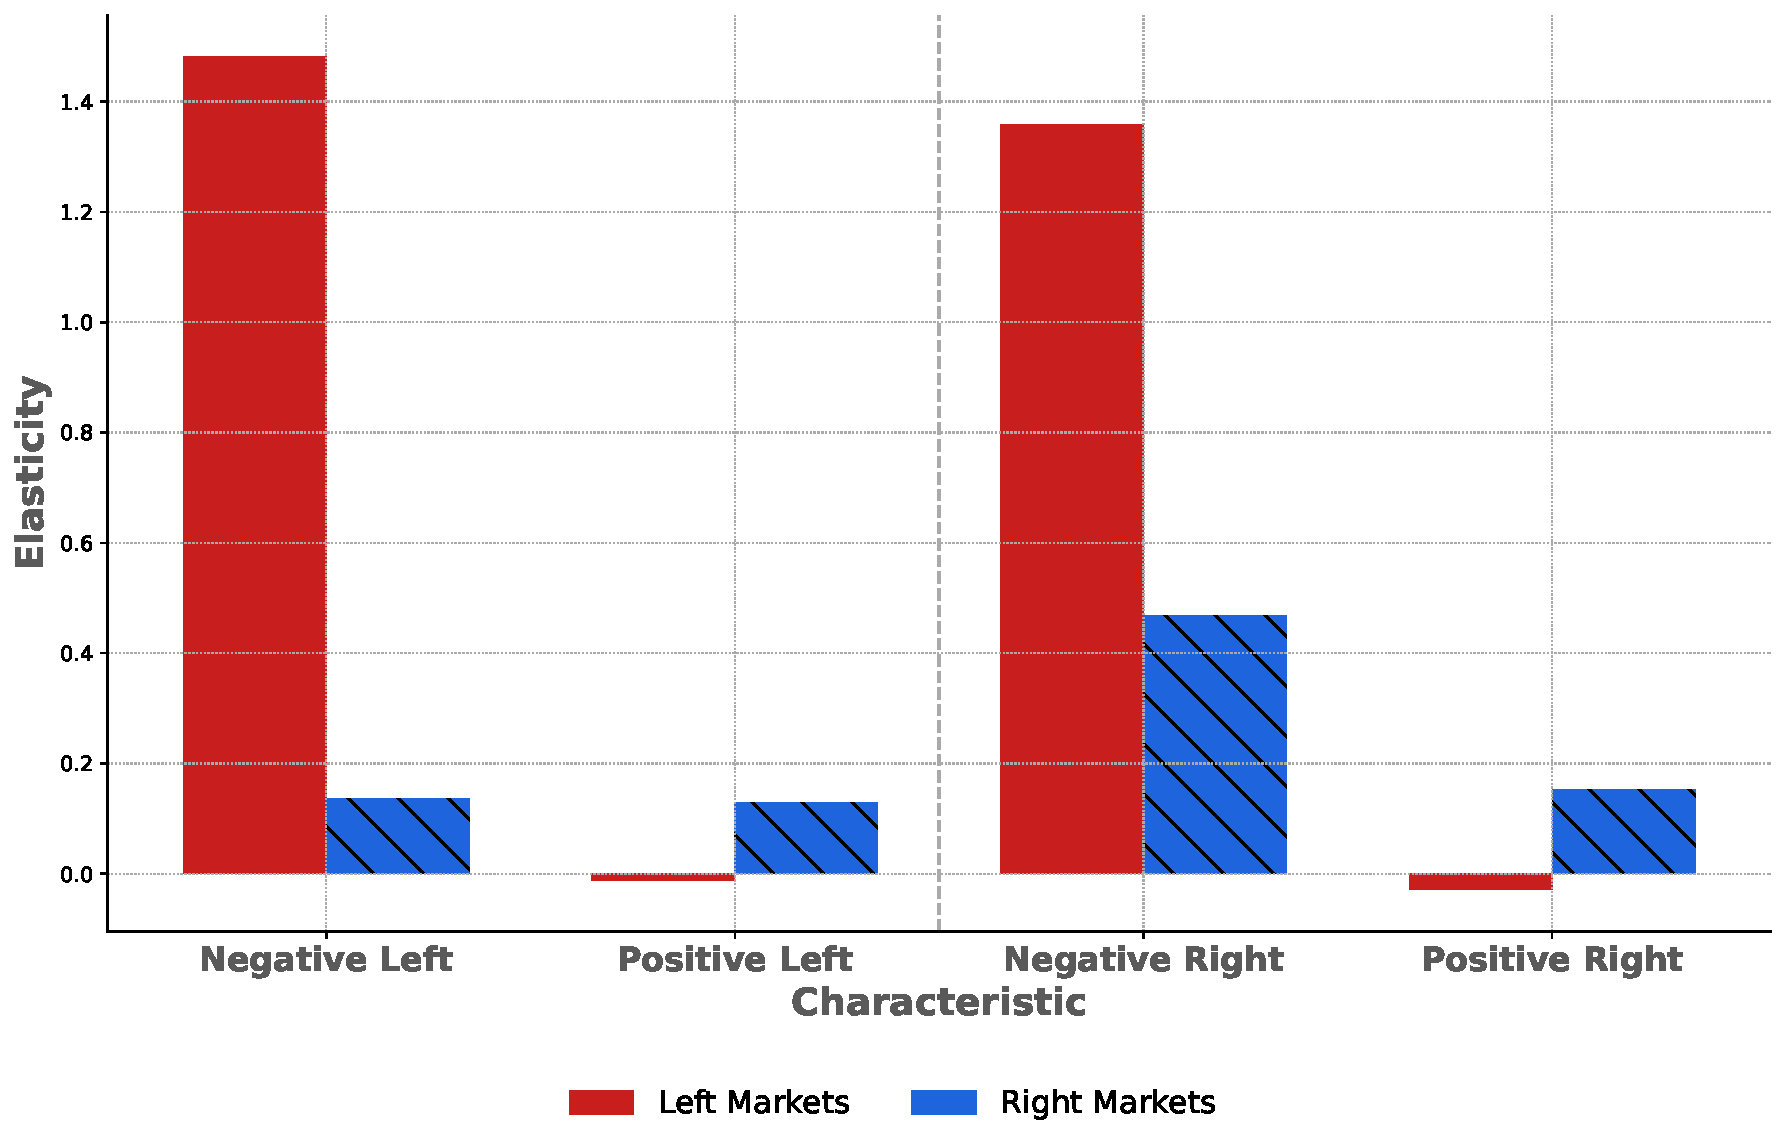
\includegraphics[width=\linewidth]{figures/elasticities_pre_campaign}
		\label{fig:2figsA}
	\end{minipage}
	\hfill
	\begin{minipage}{0.45\textwidth}
		\centering
		\textbf{(b)} Campaign\\
		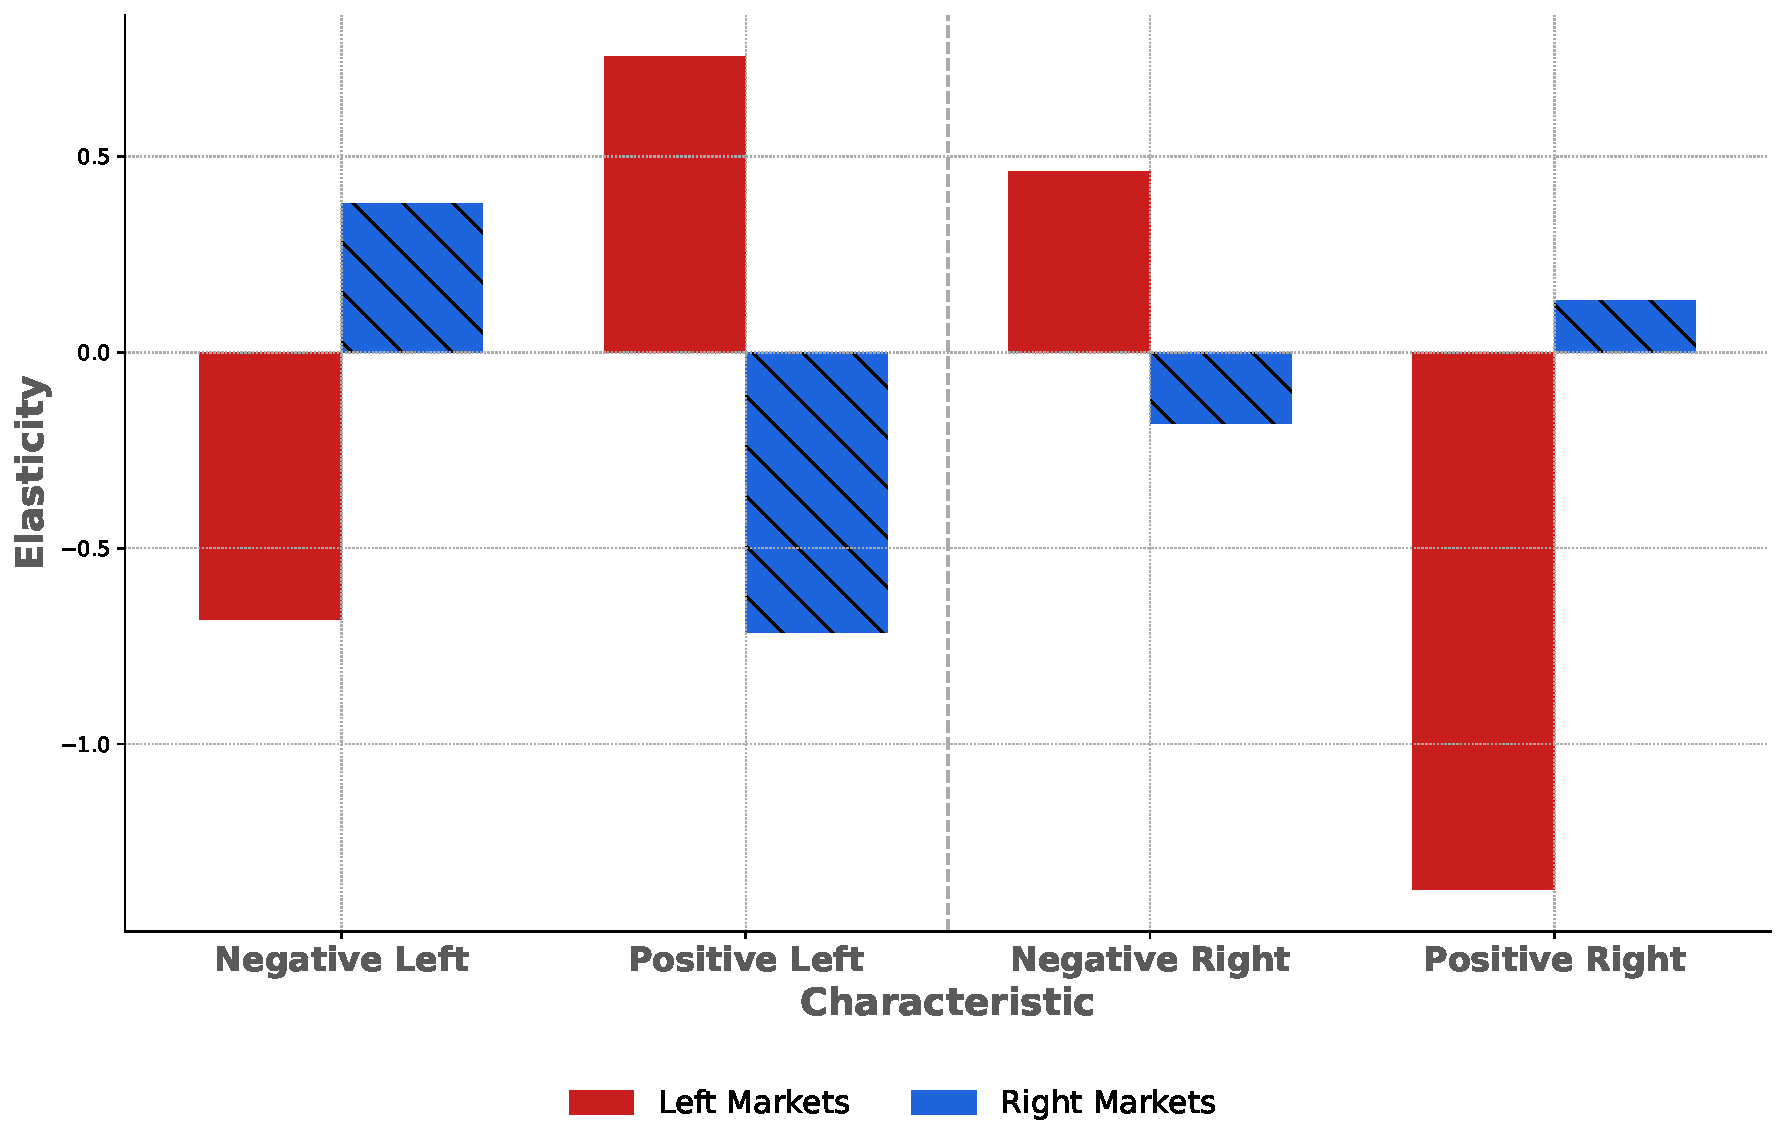
\includegraphics[width=\linewidth]{figures/elasticities_campaign}
		\label{fig:2figsB}
	\end{minipage}
	
	\vspace{0.5em} % space between figures and note
	
	\captionsetup{justification=justified}
	\caption*{\textit{Note:} \small Each panel shows estimated elasticities for consumer responses in right- and left-leaning markets. Panel (a) reports results for the pre-campaign period, while Panel (b) covers the campaign period.}
\end{figure}







	\section{Supply Side: Work in progress}
	
	\label{sec:supply}



	
	In this section, I model the channels' editorial decisions. The following quote by A3 news director Vicente Vallés clearly illustrates their slant decision process. 
	\begin{quote}
		``Even in a news program, it’s deeply subject to the daily variation of audiences [...] A drop of half a point when tackling a current issue can provoke the decision not to revisit that topic... simply because audience is lost, and thus, profitability.''
	\end{quote}
	\hspace*\fill{\small -- Vicente Vallés, Director and presenter of Antena 3 TV News, 2014\footnote{Source: \href{https://cadenaser.com/ser/2014/12/03/television/1417630810_539829.html}{https://cadenaser.com/ser/2014/12/03/television/1417630810\_539829.html}}}
	
Two important facts emerge from this quote. First, even though adds do not directly appear during the news slot; profitability is a key driver in their decisions. Outlets want to retain as much as audience as possible for the next slots. Second, their content choice decisions are done in a high frequency basis: Journalists meet every day and consider both the audience numbers and the events of the day in order to make their editorial lines. 
	
	Under that motivation, I model 	the maximization problem for a  given channel $j$ on  day $d$ is:
	
	\begin{equation}\label{eq:payoffs}
		\begin{aligned}
			\max_{\{\mathbf{x}_{jd}\}}   & \left\{   \sum_{r}s_{jrd+1}(\bm{x}_{jd}, \bm{x}_{-jd})\frac{L_r}{L} - \sum_k {\lambda^k}\mathcal{C}({x}^k_{jd}, {z}^k_d)+ \bm{\eta}_{jd}\bm{x}_{jd} \right\}\\
			s.t.   \quad &   x_{jd}^{L+} +x_{jd}^{R+} + x_{jd}^{L-} + x_{jd}^{R-} + x_{jd}^{\emptyset} = x_{jd}^{political}\\
			& x_{jd}^k \in [0,1] \quad \forall k
		\end{aligned}
	\end{equation} 
	
	
Channels want to retain maximum amount of audience over all the regions :$\sum_{r}s_{jrd+1}(\bm{x}_{jd}, \bm{x}_{-jd})\frac{L_r}{L} $ who has preferences over the content they offered on that day:  $\mathbf{x}_{jd}$. I model a simple functional form $ \mathcal{C}({x}_{jd}^k, {z}_d^k) = \frac{(x_{jd}^k) ^2}{z_d^k}$ where the inverse of the available stories acts analogously to input prices. The goal is to estimate each of the parameters $\lambda^k$ that controls for the asymmetric production costs of each type of content. 

	
Production of content also depends on the news landascape trhough  $C(\cdot)$. Under $\lambda >0$, the more stories of a type there are available on a given day, i.e high $z_d^k $ , the cheaper it is for them to produce them. These costs can have been already suggested but not estimated in previous works \citep{SimonovRao2022}.  On the other hand, if channels act as news aggregators a higher volume of stories could also increase costs since they need to read and filter what they will actually show. In this case $\lambda<0$ would indicate an \textit{informational filtering} type of cost with an inverse relation between the volume of stories and their production. The sign of $\lambda$ is therefore not clear ex-ante. 

Key for identification is the timing of preferences as outlined in the demand estimation. Audience preference for which channel to start watching the news is driven by the content presented on the previous day, since viewers have not yet been exposed to the current day’s content. Since outlets must decide which content to offer on a given day based solely on audience information from the previous day, there is no simultaneity in their editorial production and audience reactions which precludes the need of demand shifters for the estimation. 


	
	The system of first order conditions is \footnote{Notice that constrains can be ignored for estimation but should be recovered when the game is used for counterfactual analysis. }:
	
		\begin{equation}
		\begin{aligned}
			&   \sum_r\frac{\partial s_{jrd+1}}{\partial x_{jd}^k}\frac{L_r}{L}  -2\lambda_j^k \frac{x_{jd}^k}{z_d^k}  +\eta^k_{jd} =0 \quad \forall j,k 
		\end{aligned}
		\label{eq:focs}
	\end{equation} 
	

	Equation \ref{eq:focs} can be estimated with GMM under $\E(\bm{\eta_d})=0$; and it is a particular case of the \textit{common coefficients} GMM estimation \citep{hayashi2000econometrics}. 
	
	  Cost parameters capture efficiency in story telling from the channels that comes from factors other than demand. \cite{boxell2022journalist} show that journalist have ideology and this is an important factor of sorting across firms. If editors hire (or retain) reporters whose ideological leanings fit the outlet’s brand, the reporter’s ideology shows up as lower marginal effort when she covers “her” side, not as a new taste term in viewers’ utility. Outlets might also enjoy higher benefits by saving in discretion and hiring journalists that are willing to work in positions in which they can advance their careers \citep{baron2006persistent}.
	  
	  
	
The estimated parameters are shown in table \ref{table:costs}. Content characteristics are grouped into content that favors the right and the left (top and bottom row blocks). Within each block coefficients coincide in sign for all the outlets. This might be a byproduct of the modeling assumption were  every channel draws from the same wire services. Idiosyncrasies in the pool of these stories might make all channels face costs or benefits in producing them. 


	
	
	\begin{table}[H]
				
		\caption{Estimated Cost Parameters ($\lambda$) by Channel and Content Type}
		
		\centering
		\begin{tabular}{lcccc}
			\toprule
			& LA6 & TVE & T5 & A3 \\
			Characteristic &  &  &  &  \\
			\midrule
			Negative Left & -0.211 & -0.345 & -0.560 & -0.305 \\
			Positive Right & -1.367 & -1.747 & -3.952 & -2.380 \\
			\hline
			Positive Left & 0.179 & 0.144 & 3.138 & 0.674 \\
			Negative Right & 0.076 & 0.144 & 1.601 & 0.299 \\
			\hline
			Political & -0.005 & -0.007 & -0.066 & -0.012 \\
			\bottomrule
		\end{tabular}
			\caption*{\textit{Note:} \small Estimated $\lambda$ from equation \ref{eq:focs}.}
	\label{table:costs}
	\end{table}




Producing both negative right and positive left content (i.e content favorable to the left) has an associated cost with positive $\lambda$ values. The left channels La6 and TVE have lower cost of production of this type compared to the right wing channel, A3.  The situation is reversed for content favorable to the right. In this case, producing this content increases the payoff of all the channels but the right wing outlet wings significantly more than the left ones. Finally, notice how the centrist Telecinco (T5) dominates the absolute values in every row.





\section{Counterfactuals}


Across Europe, broadcast regulators increasingly impose proportional-air-time rules to curb partisan imbalances in election coverage: France’s ARCOM stopwatches every political segment to enforce strict minute-for-minute equality during the “période officielle”; Italy’s Par Condicio law compels both public and private stations to “balance and compare” exposure for all lists; and Germany grants each registered party free television slots whose length scales with its prior vote share. Spain, by contrast, still relies on a voluntary pluralism. The public network TVE issues a proportional airtime manifesto while commercial groups—Atresmedia and Mediaset—entirely unconstrained. 

My model estimates allow to test what would be the implications of enforcing such policy to all the broadcasters.  I take the proportion of votes in the past general elections for each party and estimate the new equilibrium under the following problem: 



\begin{equation}\label{eq:payoffs2}
	\begin{aligned}
		\max_{\{\mathbf{x}_{jd}\}}   & \left\{   \sum_{r}s_{jrd+1}(\bm{x}_{jd}, \bm{x}_{-jd})\frac{L_r}{L} - \sum_k {\lambda^k}\mathcal{C}({x}^k_{jd}, {z}^k_d)+ \bm{\eta}_{jd}\bm{x}_{jd} \right\}\\
		s.t.   \quad &   \frac{x_{jd}^{R+} + x_{jd}^{R-} }{x_{jd}^{political}}=vote^R\\
		&  \frac{x_{jd}^{L+} + x_{jd}^{L-} }{x_{jd}^{political}}= vote^L\\
		& x_{jd}^k \geq 0 \quad \forall k
	\end{aligned}
\end{equation} 


where I assume that time to a political party can only be discerned if that story has some specific slant and that all outlets must devote the proportion of political time given by previous proportions of votes $(vote^R, vote^L)$ (i.e constraints bind). 


\clearpage

	
	\section{Conclusion}
	
	Understanding the demand of political information is crucial to understand political polarization and media market regulation. However, endogeneity concerns often  impede classical demand estimation techniques due to the lack of valid instruments. In this paper,  I introduce a novel dataset that comprises the Spanish TV market, where I match daily transcripts of the TV news to audimeter data on viewership. I propose a new methodology that makes uses of text analysis and Large Language Models (LLMS ) to analyze the production of political content in TV news. This methodology extracts the political tone and intensity of the daily TV news and  exploits the random availability of political events, together with channel's long-run ideological positions, to measure supply shocks that allow the estimation of  demand preferences.
	
	I show that channels face asymmetric constraints  in their production of political content depending on whether the composition of the day is more or less favorable to their ideological stance. I estimate a structural BLP demand model where I split my sample into both pre-campaign and during political campaign periods. This model allows me to introduce heterogeneity into the demand estimation and decompose political preferences based on the  ideological composition of the audience. My results reveal that while there is no significant asymmetric demand for political content during the pre-campaign period, affective polarization emerges during the political campaign, with right-wing viewers demanding more negative content about the opposing party and more favorable content about their own. Finally, I model the competition game into channels' daily content production and estimate their cost structures. Right wing media enjoy higher benefits/costs on producing content that goes against their editorial line.
	
	
	
	
	
	\clearpage
	
	\section{Appendix}
	
	
	
	
	
	
	
	
	
	
	\subsection{Figures}
	
	
	
	\textbf{Pipeline}:
	
	\begin{figure}[H]
		\centering
		\caption{Pipeline for content downloading and classification }
		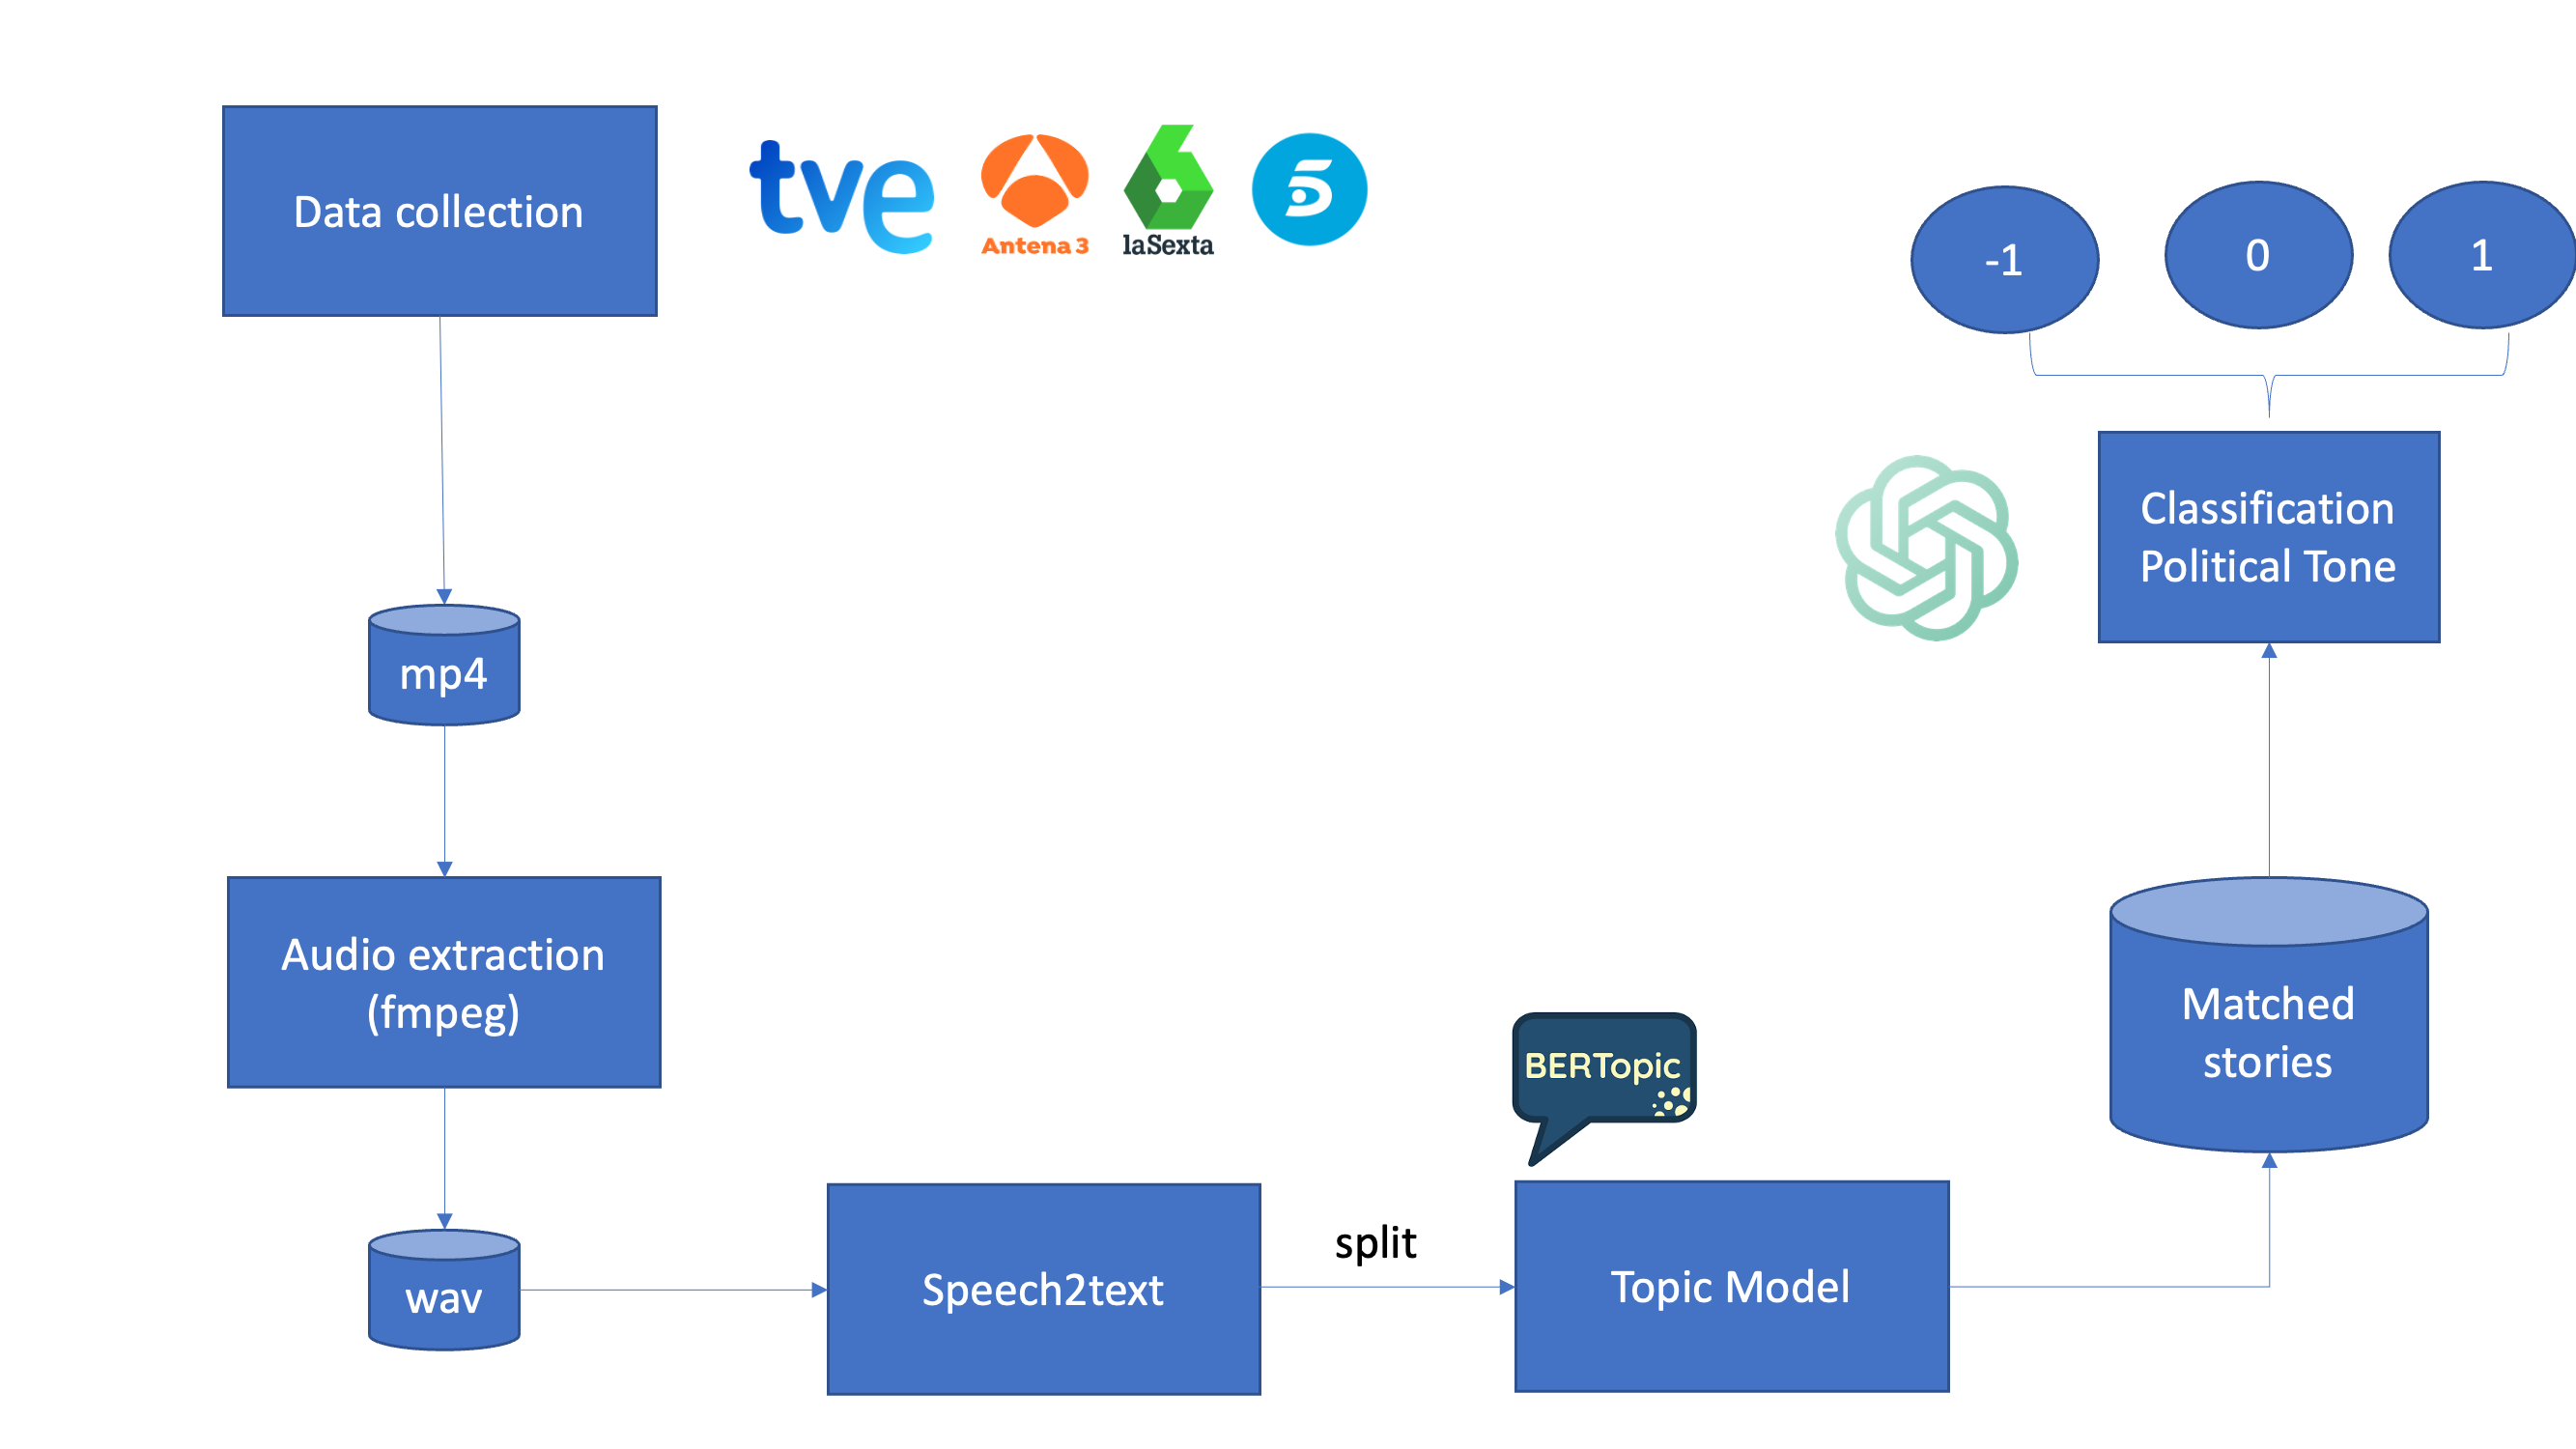
\includegraphics[width=150mm]{figures/pipeline3}
		\caption*{\small Notes: Pipeline for the text downloading. First videos are downloaded daily from the main TV channels. Google engine is used to convert the audio to text. I then split the stories by minute and user BERTopic to classify and match them. Finally, ChatGPT4 is used to classify political tone.}
		\label{fig:pipeline}
	\end{figure}
	
	
	
	
	\begin{figure}[H]
		\centering
		\caption{Box plot for TV dominance across countries and age cohorts}
		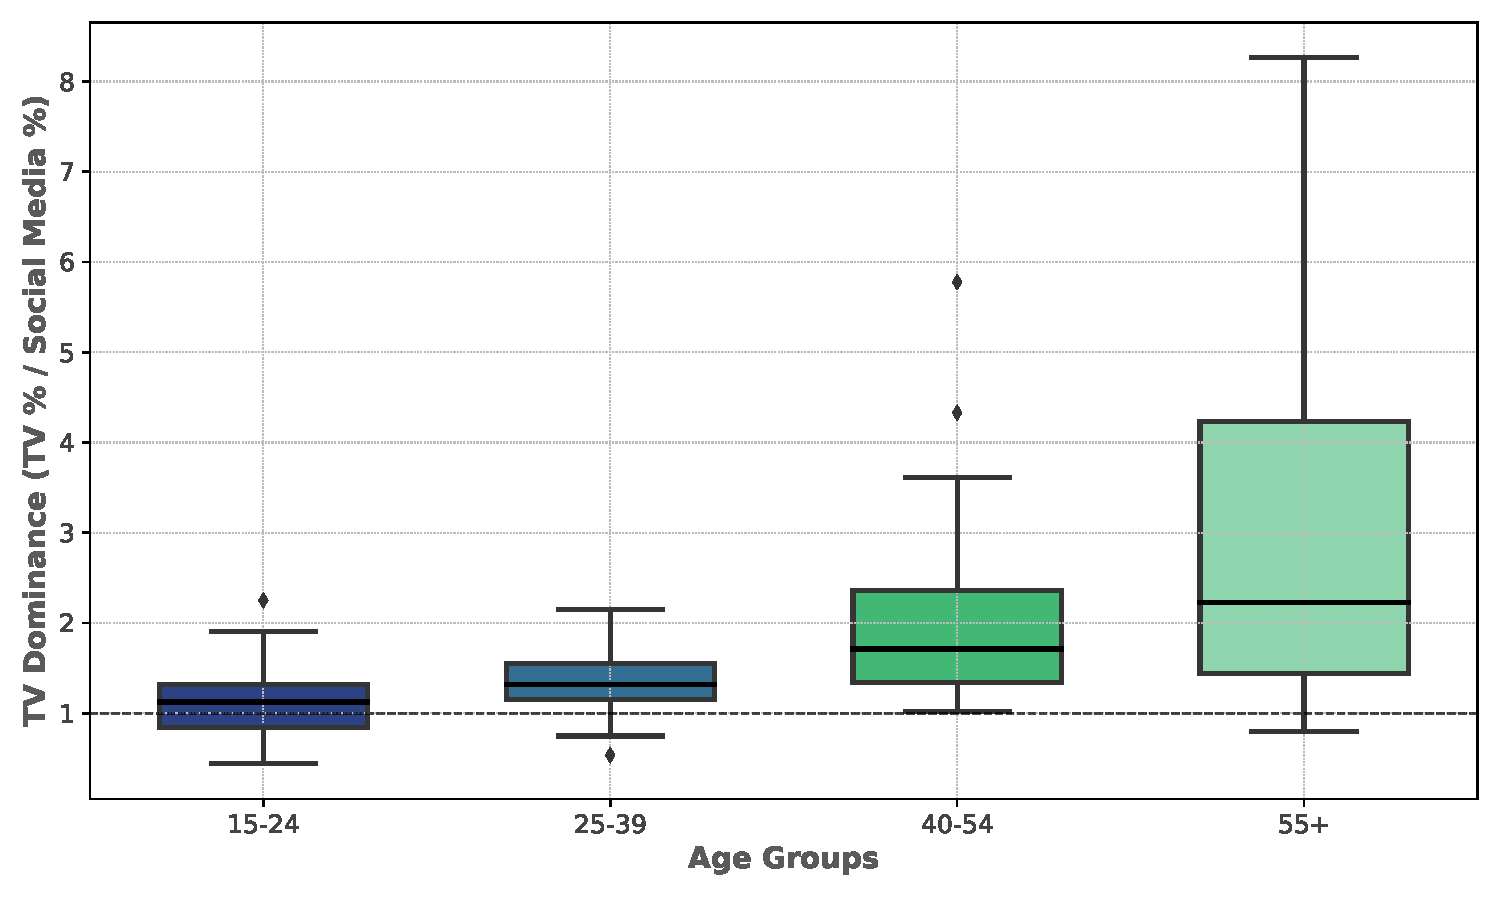
\includegraphics[width=120mm]{figures/age_cohorts_full}
		\caption*{\small Notes: Box plot of the relative TV dominance relative to social media by age cohorts. Using data for the 27 countries in Eurobarometer with $N=112059.$ Relative dominance is calculated as the total number of respondents that mark TV as the main source for political information relative to those that mark social media. 
			Source: Eurobarometer, 2022. }
		\label{fig:motivation2}
	\end{figure}
	
	\begin{figure}[H]
		\caption{Net sentiment across channels and parties pre and during campaign }
		\centering
		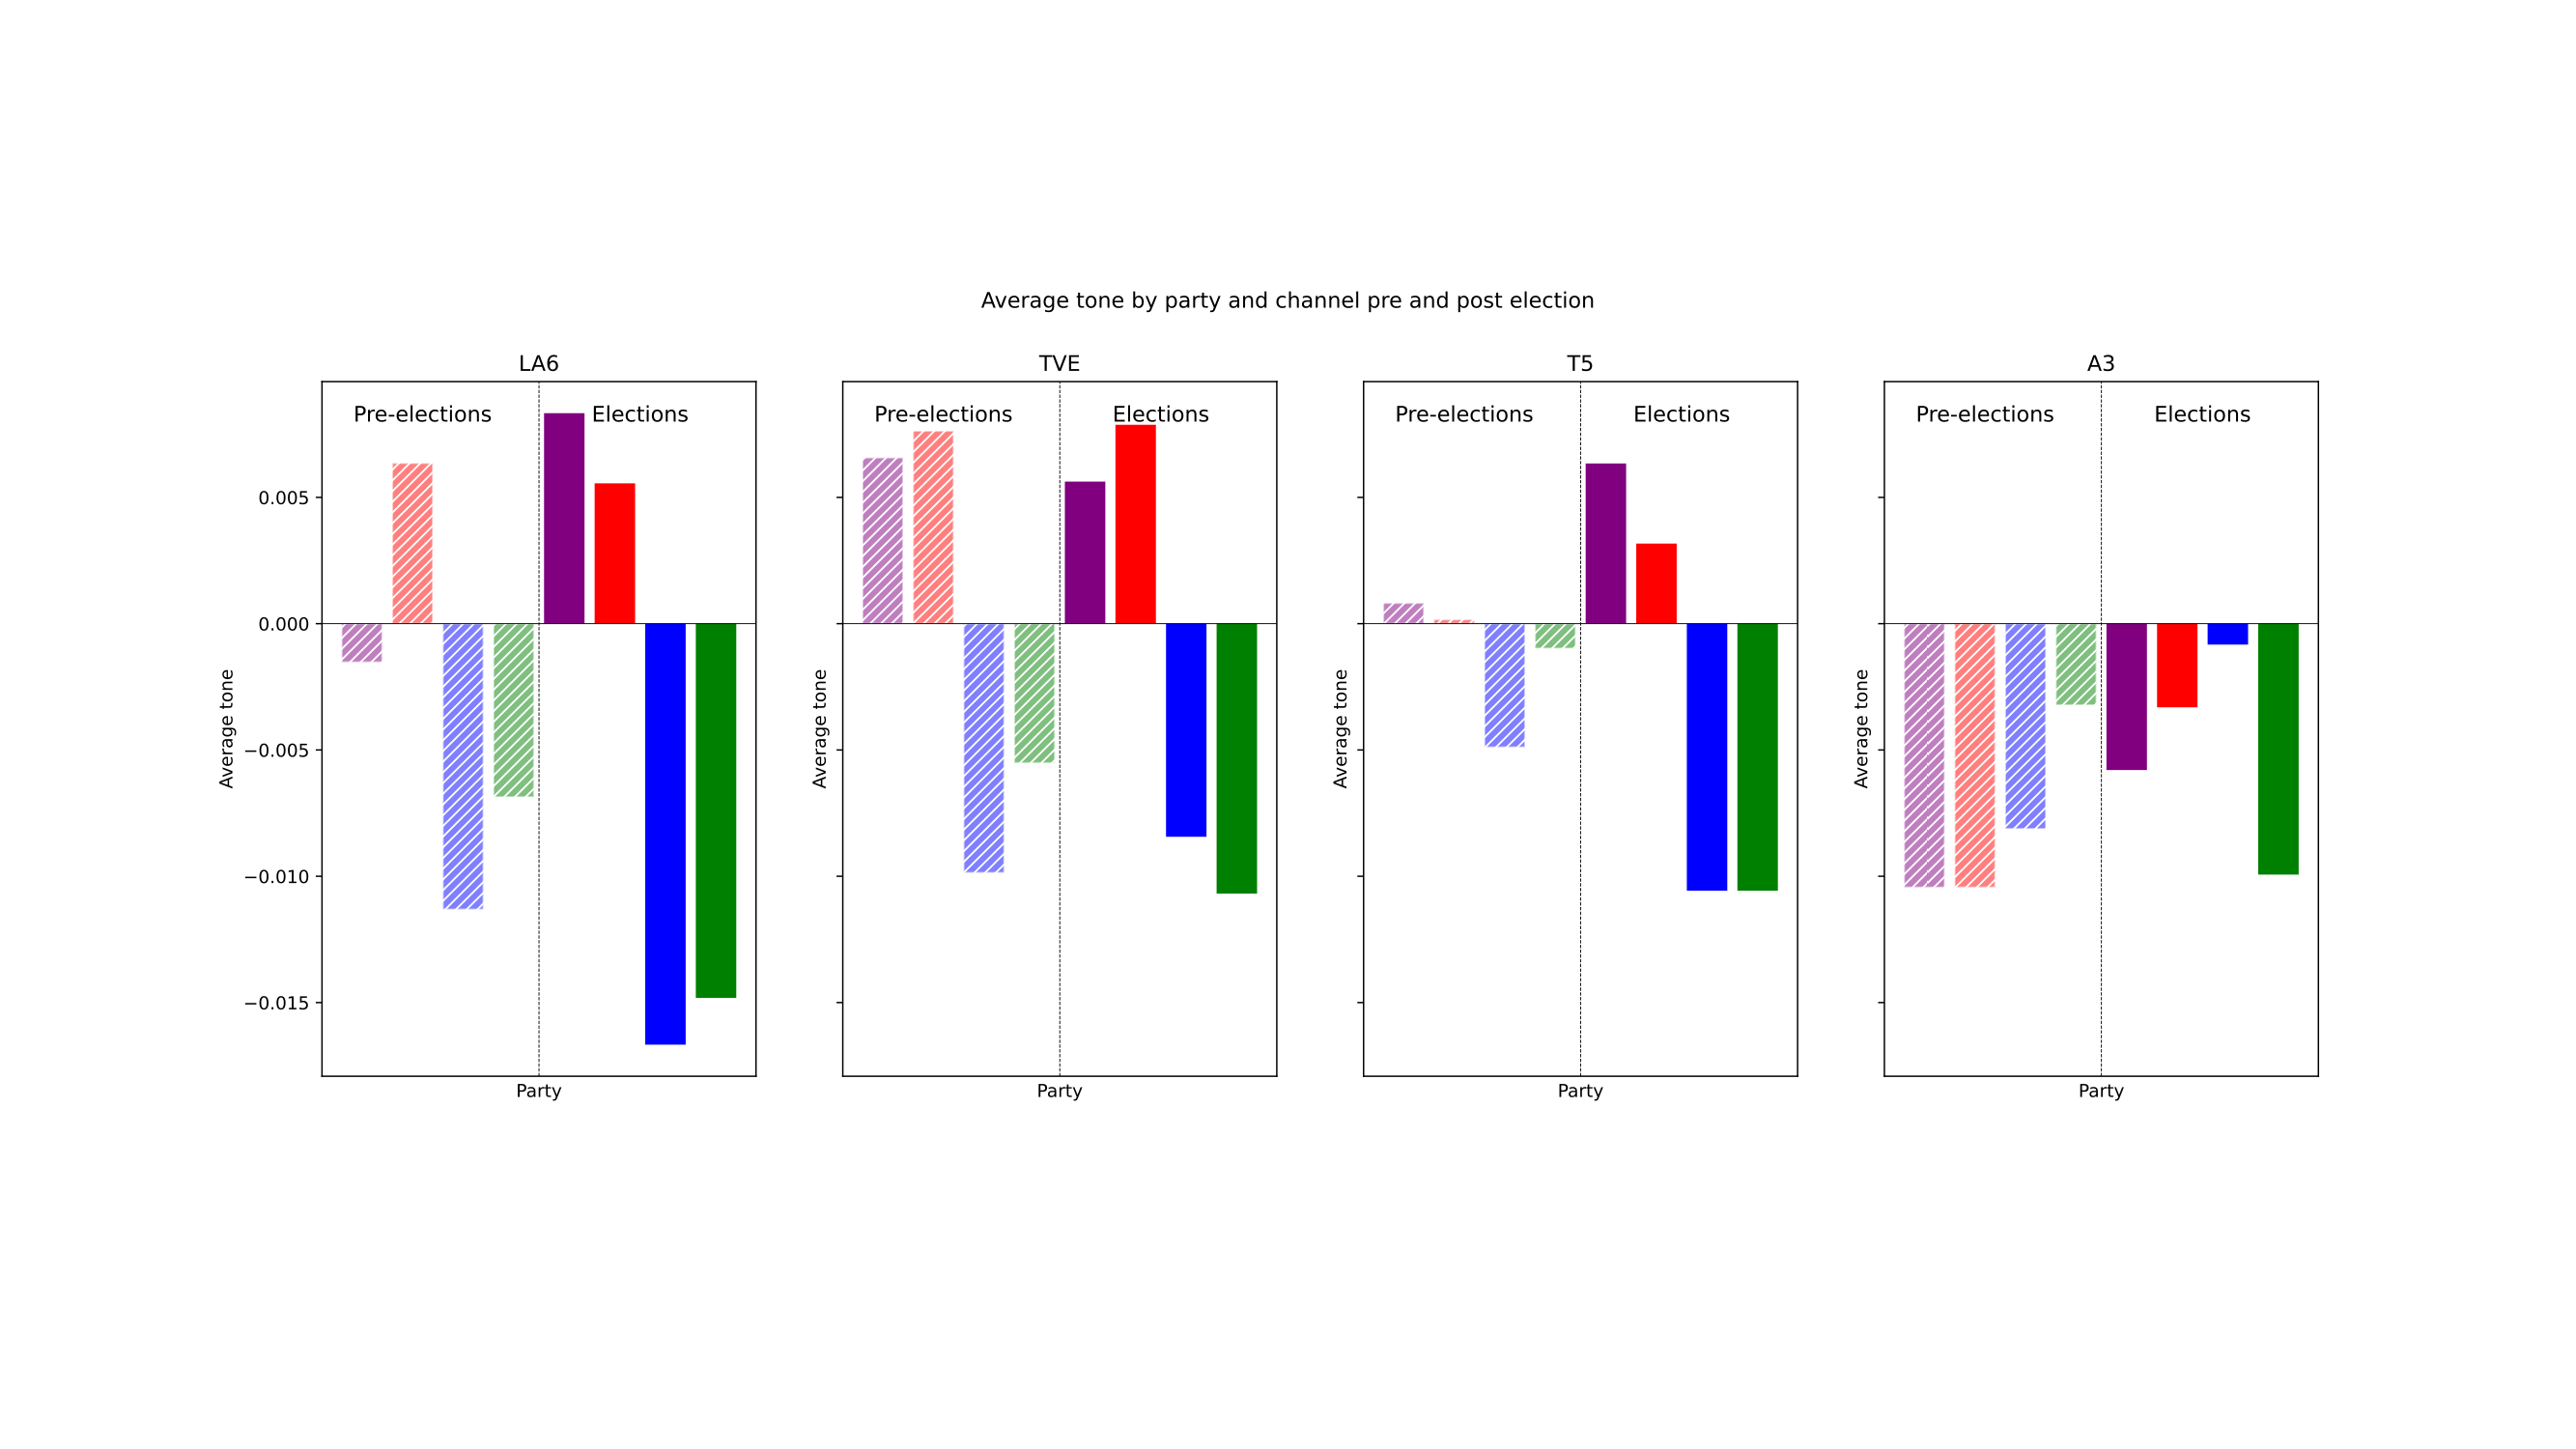
\includegraphics[width=150mm]{figures/average_tone_pre_post_election}
		\caption*{\small Notes: The figure shows the relative tone calculated as the average sentiment over right and left parties. The vertical dashed line delimits results pre and during campaign periods, respectively. }
		\label{fig:tone2}
	\end{figure}
	
	\begin{comment}
	
	\begin{figure}[H]
		\centering
		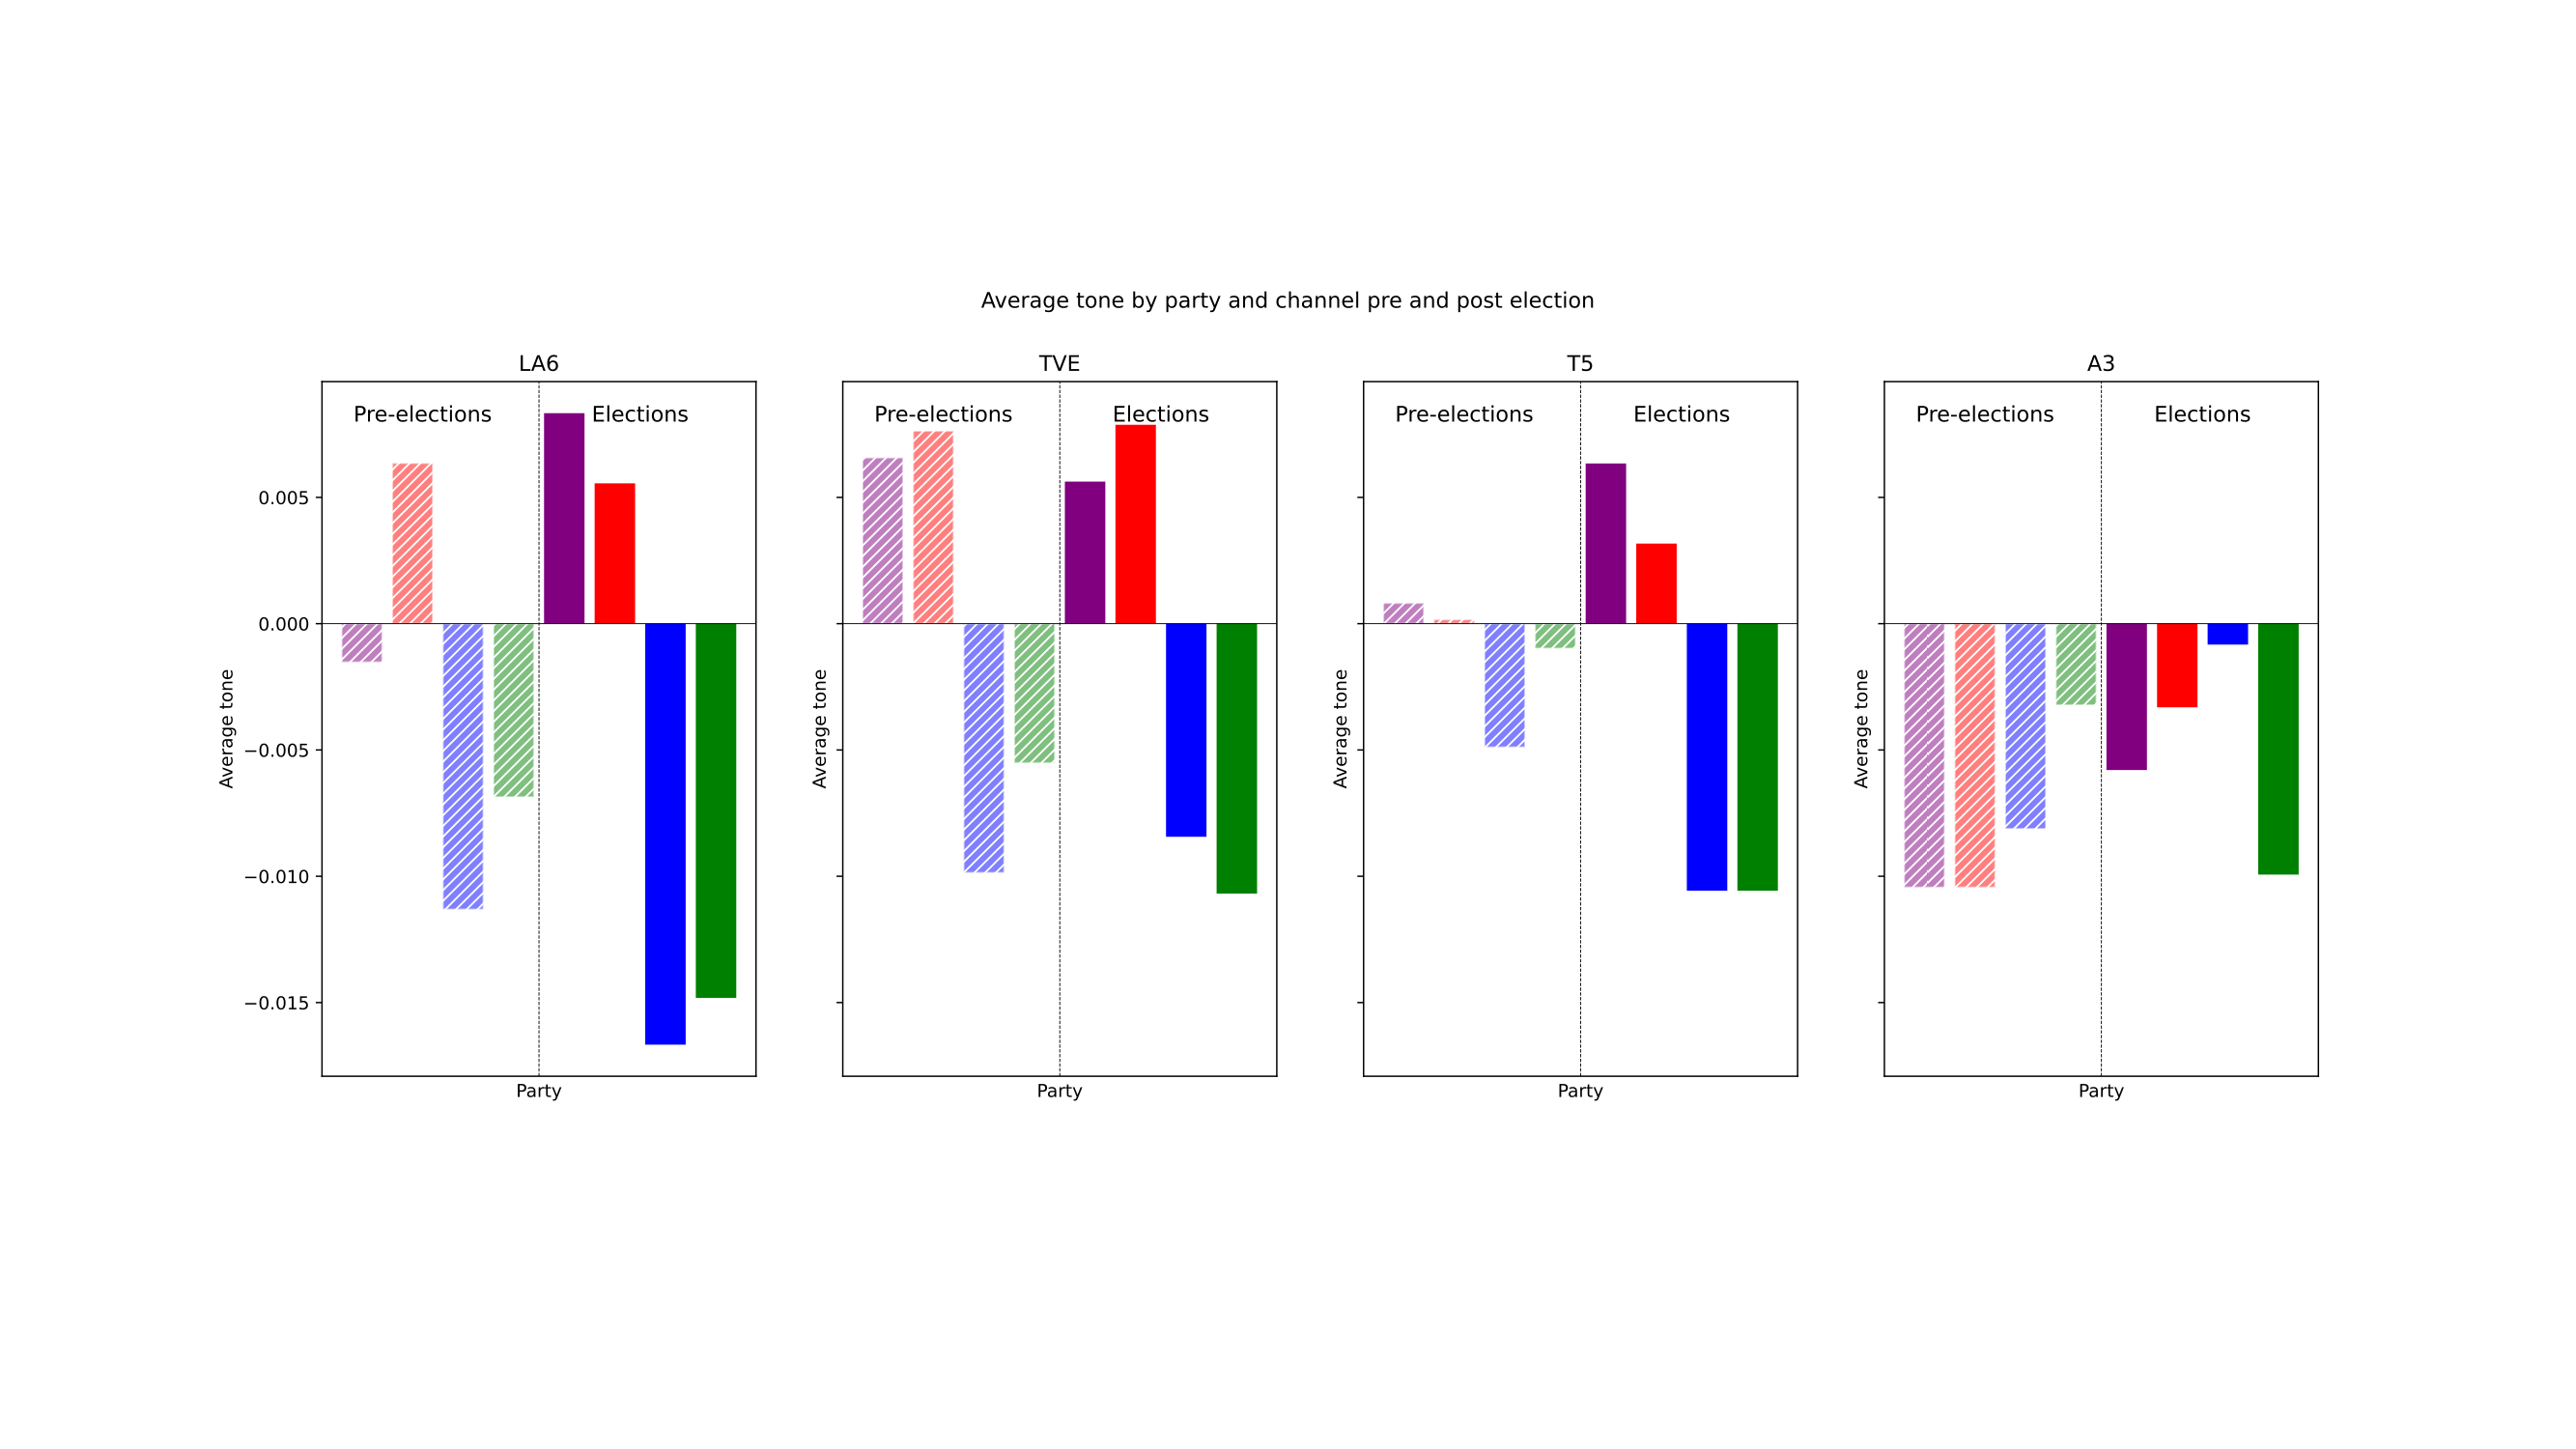
\includegraphics[width=160mm]{figures/average_tone_pre_post_election.png}
		\caption{Average tone for each party and channel pre and during campaign periods}
		\label{fig:party_decomposition}
\end{figure}
	\end{comment}	
	
	
	\begin{figure}[H]
		\centering
		\caption{Density estimation for channels ideology based on audience share data}
		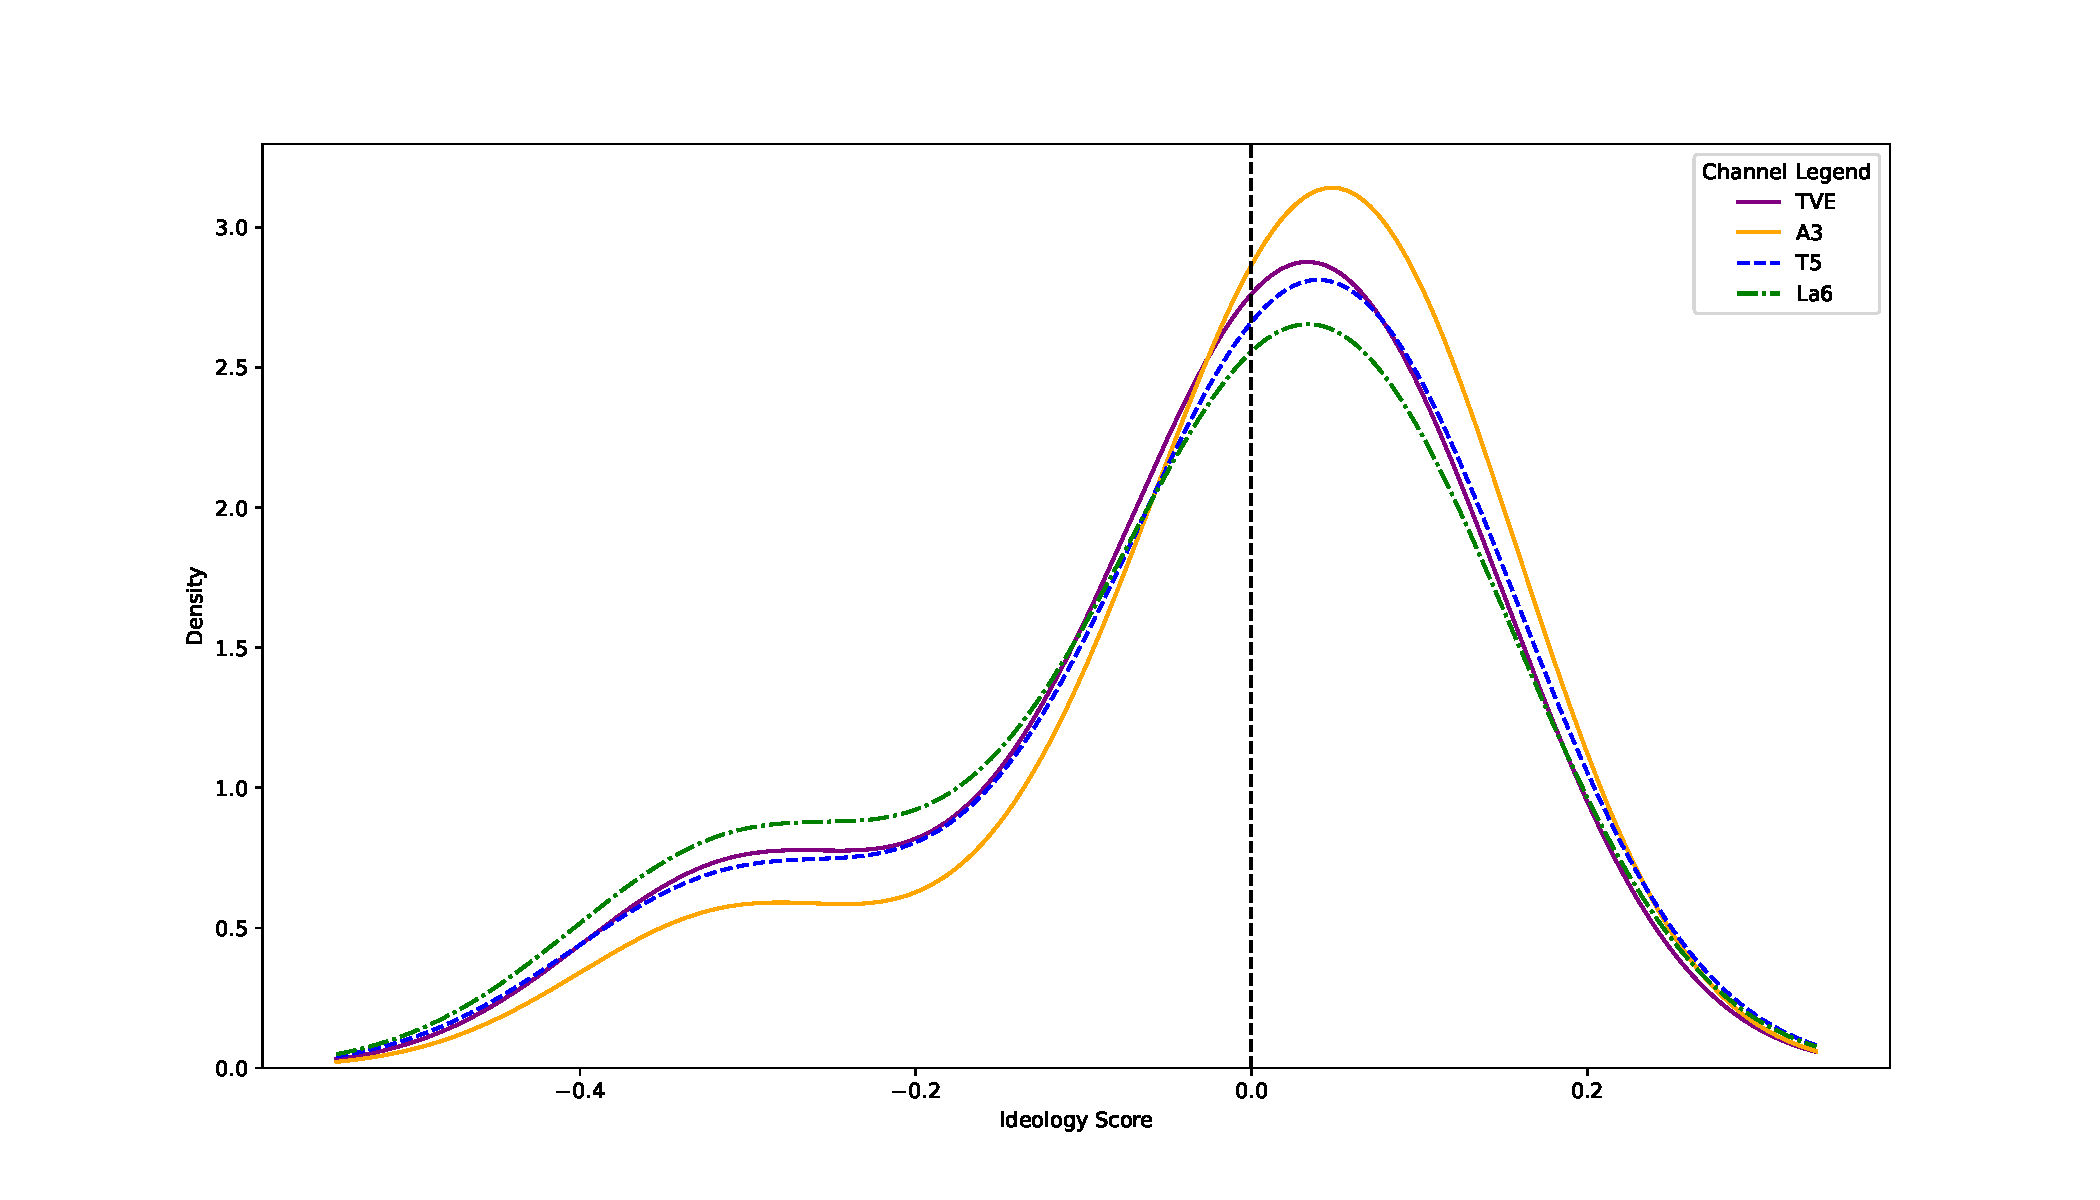
\includegraphics[width=120mm]{figures/channel_ideology_density_python}
		\caption*{\small Notes: Estimated density of channels' audience ideology. The figure shows a kernel density estimate on the ideology score constructed using survey daa and weighted by channels' share of audience for each autonomous region. }
		\label{fig:density}
	\end{figure}
	
	
	
	
	
	\clearpage
	
	\subsection{Tables}
	
	
	
	
\begin{table}[h!]
	\centering
	\caption{Top 5 Topics by party-tone category on Agencia EFE after BERTopic. }
	\begin{tabular}{|l|c|}
		\hline
				\multicolumn{1}{|c|}{\textbf{Topic Words}}& \textbf{Count} \\
		\hline
		\hline
		\multicolumn{2}{|c|}{\textbf{Positive Right}} \\
		\hline
		vox, motion, abascal, censure, pp, tamames, santiago, garriga, parties, party & 312 \\
		feijóo, núñez, alberto, pp, leader, gamarra, parties, party, general, cuca & 113 \\
		guardiola, extremadura, mérida, maría, vara, extremeño, council, assembly, candidate & 68 \\
		mazón, valencian, president, corts, valencian, valencians, government, carlos & 64 \\
		electoral, elections, general, jec, board, campaign, 28m, 23j, vote & 63 \\
		\hline
		\multicolumn{2}{|c|}{\textbf{Negative Right}} \\
		\hline
		vox, motion, abascal, censure, pp, tamames, santiago, garriga, parties, party & 369 \\
		abortion, castilla, healthcare, anti-abortion,pregnancy, abortions, law, mañueco & 112 \\
		code, criminal, sedition, embezzlement, reform, crime, penalties, amendments & 81 \\
		electoral, elections, general, jec, board, campaign, 28m, 23j, vote & 71 \\
		sánchez, pedro, feijóo, president, government, núñez, leader, alberto, pp, executive & 69 \\
		\hline
		\multicolumn{2}{|c|}{\textbf{Positive Left}} \\
		\hline
		yes, only, reform, sexual, law, is, violence, reform, just, podemos & 200 \\
		sánchez, pedro, feijóo, president, government, núñez, leader, alberto, pp, executive & 183 \\
		yolanda, díaz, vice president, sumar, second, podemos, labor, leader, minister & 179 \\
		sumar, podemos, errejón, iu, íñigo, yolanda, parties, coalition, díaz, left-wing & 142 \\
		psoe, socialists, federal, secretary, parties, socialist, lobato, espadas, congress & 129 \\
		\hline
		\multicolumn{2}{|c|}{\textbf{Negative Left}} \\
		\hline
		yes, only, reform, sexual, law, is, violence, reform, just, podemos & 182 \\
		sánchez, pedro, feijóo, president, government, núñez, leader, alberto, pp, executive & 153 \\
		vox, motion, abascal, censure, pp, tamames, santiago, garriga, parties, party & 129 \\
		sexual, assault, sexually, sexual, minor, violence, assault, convicted, abuse & 108 \\
		psoe, socialists, federal, secretary, parties, socialist, lobato, espadas, congress & 72 \\
		\hline
	\end{tabular}
	\caption{Table shows the top 5 topics associated with the top stories that provided more positive/negative coverage for each party in the Agencia EFE corpus. words were translated to English with the help of ChatGPT. }
\end{table}

	
	
	
		\begin{table}[h!]
		\centering
		\begin{tabular}{p{0.8\textwidth}}
			\toprule
			\textbf{Top stories for  Negative Left}  \\
			\midrule
			-Reduction of a convicted rapist’s sentence in Salamanca under the "Solo sí es sí" law  \\
			-Seville Court reduces a murder and sexual assault sentence by 5 years due to the "Solo sí es sí" law  \\
			-Vox formally submits a motion of no confidence against Prime Minister Pedro Sánchez  \\
			-Madrid’s regional president, Isabel Díaz Ayuso, predicts that the "Mediator Case" will bring down the government  \\
			\bottomrule
		\end{tabular}
		\begin{tabular}{l c}
			\toprule
			\textbf{Channel} & \textbf{Proportion of Negative Left} \\
			\midrule
			TVE & 0.037 \\
			Antena 3  & 0.184 \\
			Telecinco  & 0.037 \\
			La Sexta  & 0.01 \\
			\bottomrule
		\end{tabular}
		\caption{Top table shows the main stories contributing to negative left content on 2023-02-27, the highest day with negative left content,  summarized and translated to English by ChatGPT. Bottom table shows the proportion of minutes devoted to negative left content per channel on the same date.}
		\label{tab:neg_left_channels}
	\end{table}
	
	
		\begin{table}[h]
		\centering
		\begin{tabular}{p{0.8\textwidth}}
			\toprule
			\textbf{Top stories for  Negative Right}  \\
			\midrule
			-Congress declarations against Ayuso over alleged "bribes" to her brother  \\
			-Marinaleda criticizes the "abusive" arrest of two residents during a protest against Vox  \\
			-The Senate rejects a PP motion on the government's alleged partisan use of the Falcon jet  \\
			\bottomrule
		\end{tabular}
	
		

		\begin{tabular}{l c}
			\toprule
			\textbf{Channel} & \textbf{Proportion of Negative Right} \\
			\midrule
			TVE & 0.074 \\
			Antena 3  & 0.038 \\
			Telecinco  & 0.067 \\
			La Sexta  & 0.148 \\
			\bottomrule
		\end{tabular}
		\caption{Top table shows the main stories contributing to negative right content on 2023-05-17, the highest day with negative right content,  summarized and translated to English by ChatGP. Bottom table shows the proportion of minutes devoted to negative right content per channel on the same date. }
		\label{tab:neg_right_channels}
	\end{table}
	
	
\begin{table}[ht]
	\centering
	\begin{tabular}{|l|l|l|}
		\hline
		Positive Right & Negative Right \\
		\hline
		secretario general vox & gürtel servicio nacional \\
		vox ignacio garriga & juicio gürtel servicio \\
		general vox ignacio & valenciana francisco camps \\
		núñez feijóo llamado & gürtel juicio gürtel \\
		candidato pp elecciones & expresidente generalitat valenciana \\
		partidos vox madrid & generalitat valenciana francisco \\
		josé sáenz buruaga & vicesecretaria general psoe \\
		núñez feijóo pedido & juicio gürtel madrid \\
		maría josé sáenz & reforma ley aborto \\
		may presidente pp & expresidente valenciano francisco \\
		\hline
	\end{tabular}
	\caption{Top trigrams for Positive Right and Negative Right on the Agencia EFE dataset using the ChatGPT categories.}
	\label{tab:top_words_pos_right_neg_right}
\end{table}
	
\begin{table}[ht]
	\centering
	\begin{tabular}{|l|l|l|}
		\hline
		Positive Left & Negative Left \\
		\hline
		agricultura pesca alimentación & tribunales ere sevilla \\
		ministro agricultura pesca & derechos sociales ione \\
		dic presidente gobierno & sociales ione belarra \\
		pesca alimentación luis & junta andalucía josé \\
		alimentación luis planas & andalucía josé antonio \\
		ene presidente gobierno & aplicación ley solo \\
		vicesecretaria general psoe & expresidente junta andalucía \\
		consejo ministros aprobado & caso mediador palmas \\
		ministra asuntos económicos & mediador palmas gran \\
		vicepresidenta primera ministra & núñez feijóo acusado \\
		\hline
	\end{tabular}
	\caption{Top trigrams for Positive Left and Negative Left on the Agencia EFE dataset using the ChatGPT categories.}
	\label{tab:top_words_pos_left_neg_left}
\end{table}
	
	
	
	
	
	
	
	
	
	\begin{table}[ht]
		\label{tab:elasticities}
		\caption{Estimated Elasticities by Left and Right markets}
		\begin{tabular}{l|cc|cc}
			\toprule
			& \multicolumn{2}{c|}{\textbf{Pre-campaign}} & \multicolumn{2}{c}{\textbf{Campaign}} \\
			Characteristic & Left Market & Right Market & Left Market & Right Market \\
			\midrule
			Negative Left & 1.481 & 0.136 & -0.681 & 0.380 \\
			Positive Left & -0.011 & 0.129 & 0.754 & -0.716 \\
			Negative Right & 1.358 & 0.469 & 0.462 & -0.182 \\
			Positive Right & -0.029 & 0.152 & -1.371 & 0.133 \\
			\bottomrule
		\end{tabular}
		\caption*{\textit{Note:} \small The table shows the average elasticities for each characteristic by right and left markets as defined in equation \ref{eq:elasticities}. Right markets are defined as regions with proportion of right wing voters above the median. }
	\end{table}
	
	\clearpage
	
	
	\subsection{Examples stories and classification}
	
	
	\begin{longtable}{|p{8cm}|c|c|c|}
		\hline
		\textbf{Story} & \textbf{Channel} & \textbf{Date} & \textbf{Sentiment} \\
		\hline
		A survey of 6,000 teenagers in Madrid schools reveals that 26\% do not identify as heterosexual, though fear of expressing it publicly is growing. Trans students represent 3\%. The Minister of Equality has called for commitment against harassment. She emphasized the importance of addressing not only positive progress but also areas where work remains, condemning normalization of hate speech... & TVE & 2023-04-14 & positive UP \\
		\hline
		In Mallorca, Unidas Podemos claims the elections are a referendum on the right to housing. They take credit for the new housing law and accuse their government partners of delaying its approval over the legislative term... & A3 & 2023-05-15 & positive UP \\
		\hline
		Pedro S\'anchez will pause his electoral campaign to attend the NATO Summit in Vilnius, following Spain's assumption of the EU Council presidency. U.S. President Joe Biden will also attend after a stop in London to meet King Charles III. & A3 & 2023-07-09 & positive PSOE \\
		\hline
		Prime Minister Pedro S\'anchez visited the command center for those affected by a wildfire, linking it to climate change and urging serious action. He announced a cabinet reshuffle, naming new ministers for Health, and Industry, Trade, and Tourism. & TVE & 2023-03-27 & positive PSOE \\
		\hline
		Regarding the Penal Code reform, the Popular Party leader called for reinstating the sedition charge, criticizing Pedro S\'anchez's decisions as ridiculous and opportunistic. & TVE & 2023-02-14 & positive PP \\
		\hline
		PP leader Feij\'oo criticized the PSOE for aligning with Podemos, suggesting a streamlined government structure with 13-14 ministries compared to the current 22. He equated PSOE's approach to that of Podemos while Pedro S\'anchez likened PP to Vox. & A3 & 2023-06-01 & positive PP \\
		\hline
		The new PP government in the Balearic Islands abolished inheritance and donation taxes for direct relatives, reduced taxes for other relatives, and lowered property transfer taxes for young first-time buyers. & A3 & 2023-07-18 & positive PP \\
		\hline
		Vox is key in provincial capitals like Valladolid, where their alliance could secure an absolute majority. Talks are ongoing in regional governments, with Azc\'on meeting Vox representatives to negotiate a coalition for Arag\'on. & LA6 & 2023-06-13 & positive Vox \\
		\hline
		Vox filed its second motion of no-confidence against the government, this time with a candidate who is not the party leader. & A3 & 2023-02-27 & positive Vox \\
		\hline
		In Extremadura, the Socialist Party risks losing its majority, while the PP and Vox could enter the regional parliament for the first time, potentially tipping the balance after the elections. & T5 & 2023-05-23 & positive Vox \\
		\hline
		On Thursday, the commission for the reform of the law begins. A reform that creates significant division between the Socialist Party and Podemos. Podemos is also facing another challenge: negotiations with Yolanda Díaz to run together in the elections. - They are still searching for a formula to run together in the general elections. And since no agreement has been reached yet, Belarra is asking Yolanda Díaz today to campaign for Podemos in the May 28 elections. & A3 & 2023-04-09 & negative UP\\
		\hline
		Here in Spain, a day after the launch of her platform, Yolanda Díaz continues exchanging criticisms with Podemos. The Podemos party did not attend, highlighting the division to the left of the PSOE. Díaz urges them to explain their absence while asserting that a "Sumar" without Podemos would not be a failure. This diagnosis contrasts sharply with that of Podemos. It remains to be seen whether, in the end, Sumar decides to proceed without Podemos. & T5 & 2023-04-03 & negative UP \\
		\hline
		The alleged extortion scheme involving former Socialist deputy Juan Bernardo Fuentes, who is under investigation. The PSOE highlights the swift action taken by the party to suspend his membership and force him to relinquish his seat.
		We need explanations, and we need them now because, with each passing day, what we learn only adds to the shame, and it keeps getting worse. & TVE & 2023-02-27 & negative PSOE \\
		\hline
		The weekend arrives after a few intense days for the governing coalition. The insults from Podemos towards the PSOE continue over their reliance on the PP to reform the "Only Yes is Yes" law. However, nothing changes, and now everyone is focusing on the campaign for the May 28 elections. & A3 & 2023-04-21 & negative PSOE\\
		\hline
		"We're going in, and we're stopping the machines." Residents of San Fernando de Henares, in Madrid, temporarily halted Metro construction works that are damaging their homes. They accuse Ayuso's government of not listening to them. Workers are injecting cement to stabilize the ground, which has shifted due to the subway extension—a measure that is cracking their walls. & LA6&  2023-01-05 & negative PP\\
		\hline
		The Supreme Court upholds the sentences handed down by the National Court to the ringleaders of the Gürtel Scheme for the embezzlement of public funds during the Pope's visit to Valencia in 2006. Francisco Correa has been sentenced to 13 years in prison for rigging contracts, Pablo Crespo to 15 years, and "El Bigotes" to 6 years. & A3 & 2023-04-10 & negative PP\\
		\hline
		But this is the strategy devised by the Madrid PP, led by Ayuso, and endorsed by the national PP under Feijóo: to raise the level of tension in the discourse to take votes away from Vox in the Community of Madrid. This is part of Ayuso's attempt to secure an absolute majority, which, according to polls, is within reach but not guaranteed.& A3 & 2023-05-18 & negative VOX\\
		\hline
		The results could be excellent. That said, like my colleagues, I must tell you that nothing is certain yet. Sumar is calling for votes to avoid a return to black-and-white. Yolanda Díaz is rallying women against the prospect of Abascal becoming vice president under Feijóo and predicts a return to an austerity-driven Spain with a right-wing government. & LA6 & 2023-07-15 & negative VOX\\
		\hline
		
		\caption{The table shows examples of fragments of stories associated with different tone for each party according to the Chat GPT classification. Stories has been translated to English with the help of ChatGPT.}
	\end{longtable}
	
	
	
	
	\subsection{Chat GPT ideology classification}\label{sec:chat_gpt}
	
	In this section I summarize the usage of ChatGPT as a text classifier for political tone. We detail the prompt and specification details used for the text classification together with final results. 
	
	
	
	
	To reduce both computational and monetary costs, I first filter our split stories using a simple dictionary based approach into those that might contain any relevant political information. Table \ref{table:politics} shows the key terms used to filter the political stories. After the match, I obtain a final number of 15406 political stories that I feed into the chat GPT classifier.
	
	\clearpage
	
	\begin{longtable}{|l|l|l|l|l|}
		\hline
		\textbf{Political} & \textbf{PP} & \textbf{PSOE} & \textbf{SUMAR/UP} & \textbf{VOX} \\
		\hline
		política & pp & psoe & unidas podemos & vox \\
		democracia & partido popular & partido socialista & podemos & abascal \\
		partido político & feijoo & sanchez & ione belarra &de los monteros \\
		gobierno & alberto nunez feijoo & federico buyolo garcia & pablo iglesias & macarena olona \\
		elecciones & ayuso & maria jesus montero & yolanda diaz & ortega smith \\
		votación & cuca gamarra & carmen calvo & irene montero & rocio monasterio \\
		constitución & pablo casado & jose luis abalos & alberto garzon & ignacio garriga \\
		legislación & esperanza aguirre & felix bolanos & iona errejon &jose alcaraz \\
		senado & ana pastor & francina armengol & monica garcia & herminio campillo \\
		congreso & pilar barreiro & sanchez mato & jaume asens & zambrano garcia \\
		dictadura & rafael hernando & margarita robles & noelia vera & luis gestoso \\
		soberanía &alvarez de toledo & marlaska & raul camargo & \\
		estado & javier maroto & jose manuel albares &lopez de uralde & \\
		ciudadanía &  & isabel rodriguez & rosa martinez & \\
		derechos &  &  &  & \\
		libertades &  &  &  & \\
		\hline
		\caption{The table shows the political words included to filter the stories into national politics. We included both general terms that refer to politics as well as party specific terms.}
		\label{table:politics}
	\end{longtable}
	
	
	
	I use OpenAI PI research  using model \textit{gpt-4-0125-preview} to build queries of the form: 
	
	
	\begin{tcolorbox}[colback=blue!5!white, colframe=blue!75!black, title=Prompt]
		Analyze the sentiment of the following news article with respect to the political parties (and their members) in Spain: PP, Podemos/Sumar, PSOE, VOX. Only use numeric values from the set [-1, -0.5, 0, 0.5, 1].
		
		Evaluate the sentiment towards each party with a number between -1 and 1, where -1 indicates an extremely negative perception, 0 indicates neutrality or irrelevance for the party, and 1 indicates an extremely positive perception.
		
		Consider only the values -1, -0.5, 0, 0.5, and 1.
		
		Base your evaluation solely on the explicit content of the news article. If the article does not mention or imply any sentiment towards a party, assign a 0 to that party.
		
		The format must always be a list \texttt{[PP
			, PSOE
			, UP
			, VOX
			]} where \texttt{X} represents the numeric sentiment value.
		
		
	\end{tcolorbox}
	
	
		\subsection{ Digression: LLMs Stability and Alternative Ideology classifications }
	\label{sec:sent_stability}
	
	
	\textbf{Stability of the classifier}
	
	Due to the stochasticity in LLMs predictions, good practices recommend to run the classification multiple times and avere out the results \citep{tornberg2023}. Financial costs, however, impede me from doing the whole approach multiple times but I show results on stability below on a random subset of  40 stories. Table \ref{tab:table_stability} shows the mean and standard dviation of the classification output for 100 rounds of classification. 
	
	Results of the final classification for the non neutral stories are shown in figure \ref{fig:sent_distribution}. Each bar represents the percentage of stories of that given sentiment associated to each political party. We can see that the classification reserved the extreme values 1 and -1 for few stories and focused on the -0.5 and 0.5 values. 
	
	
	\begin{table}[H]
		\centering
		\caption{Mean and Standard Error for 100 Rounds of ChatGPT Classification}
		\begin{tabular}{|l|c|c|c|c|}
			\hline
			\textbf{Statistic} & \textbf{PP} & \textbf{PSOE} & \textbf{VOX} & \textbf{UP} \\
			\hline
			Mean & -0.014 & 0.106 & -0.053 & 0.024 \\
			Standard Error & 0.003 & 0.004 & 0.001 & 0.002 \\
			\hline
		\end{tabular}
		\caption*{Note: The table shows the mean and standard error for 100 rounds of ChatGPT classification of political content with 40 random political stories.}
		\label{tab:table_stability}
	\end{table}
	
	
	\begin{figure}[H]
		\centering
		\caption{ChatGPT distribution of scores for each political party}
		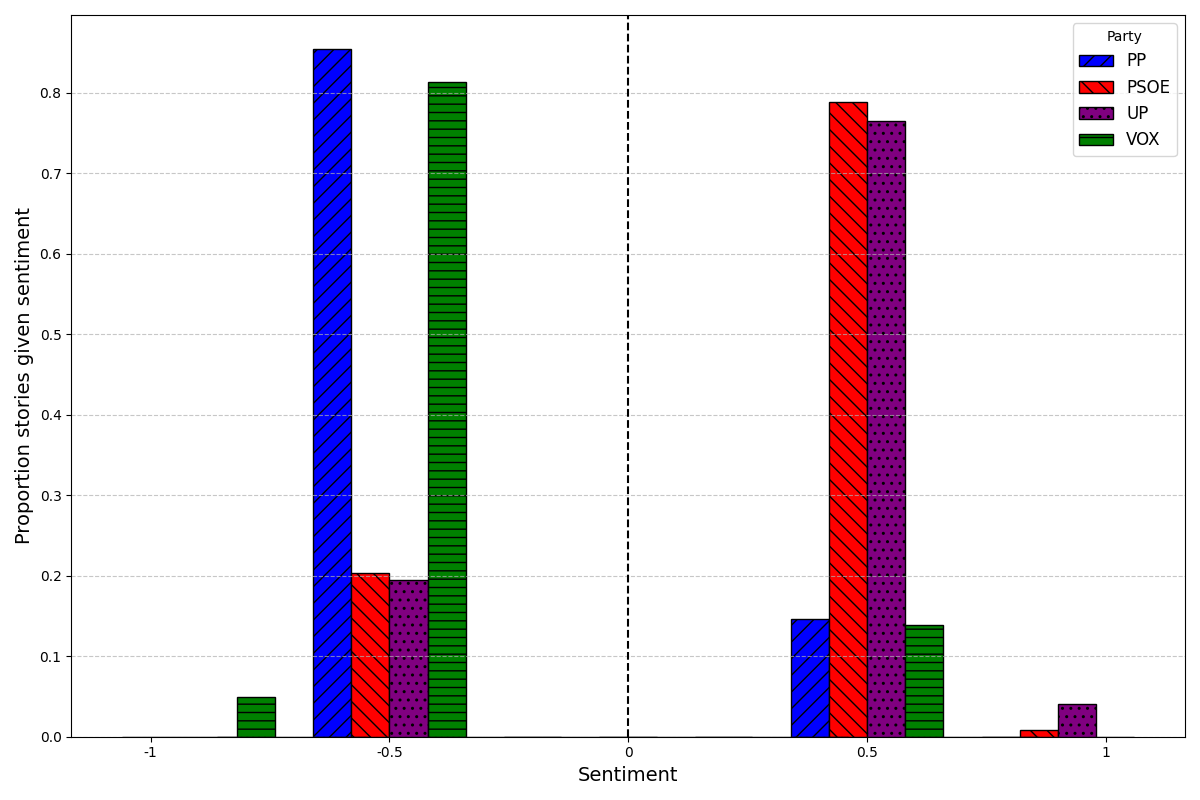
\includegraphics[width=120mm]{figures/sentiment_distribution}
		\caption*{\small Notes: The figure shows the percentage of stories to each political party for a given sentiment. We exclude neutral stories.}
		\label{fig:sent_distribution}
	\end{figure}
	
	\textbf{Alternative ideology classification}
	
	
Similar to \cite{gentzkow2010media} and \cite{laver2003extracting} I exploit party ideology in congress speeches to calculate similarity measures of the outlet's speech. I make use of all congressional speeches produced during my sample period and associate each speaker with their respective political party, filtering to retain the set of relevant parties.

I follow a similar, non-linear version of \cite{laver2003extracting} and create a score for each word $w$ in the congress speech as: 


	
	\begin{equation}
		\text{Score}(w) \;=\; \ln \left( \frac{\mathrm{freq}(w,\text{Left}) + \alpha}{\mathrm{Total}_{\text{Left}} + \alpha} \right) \;-\; \ln \left( \frac{\mathrm{freq}(w,\text{Right}) + \alpha}{\mathrm{Total}_{\text{Right}} + \alpha} \right),
		\label{eq:log_ratio}
	\end{equation}
	
	where:
	\begin{itemize}
		\item $\mathrm{freq}(w,\text{Left})$ is the number of times word $w$ appears in the speeches of left-leaning parties (PSOE and UP),
		\item $\mathrm{Total}_{\text{Left}}$ is the total word count in left-party speeches,
		\item $\mathrm{freq}(w,\text{Right})$ and $\mathrm{Total}_{\text{Right}}$ are defined analogously for right-leaning parties (PP and Vox), and
		\item $\alpha$ is a small smoothing parameter.
		
	\end{itemize}
	
	I select the value of alpha that maximizes accuracy of label prediction in the congress dataset; $\alpha=0.9$.	
	Words with high positive scores are used disproportionately in left-leaning speeches, while those with high negative scores are more characteristic of right-leaning speeches. I rank all words by their computed score and select the top 100 left-coded words and top 100 right-coded words, represented in wordcloud figures  \ref{fig:worcloud1} and \ref{fig:worcloud2}.
	

	
	
	
	
	\begin{figure}[H]
		\centering
		\begin{minipage}{0.46\textwidth}
						\label{fig:wordcloud1}
						\captionof{figure}{Word Cloud Top Left Words}
			\centering
			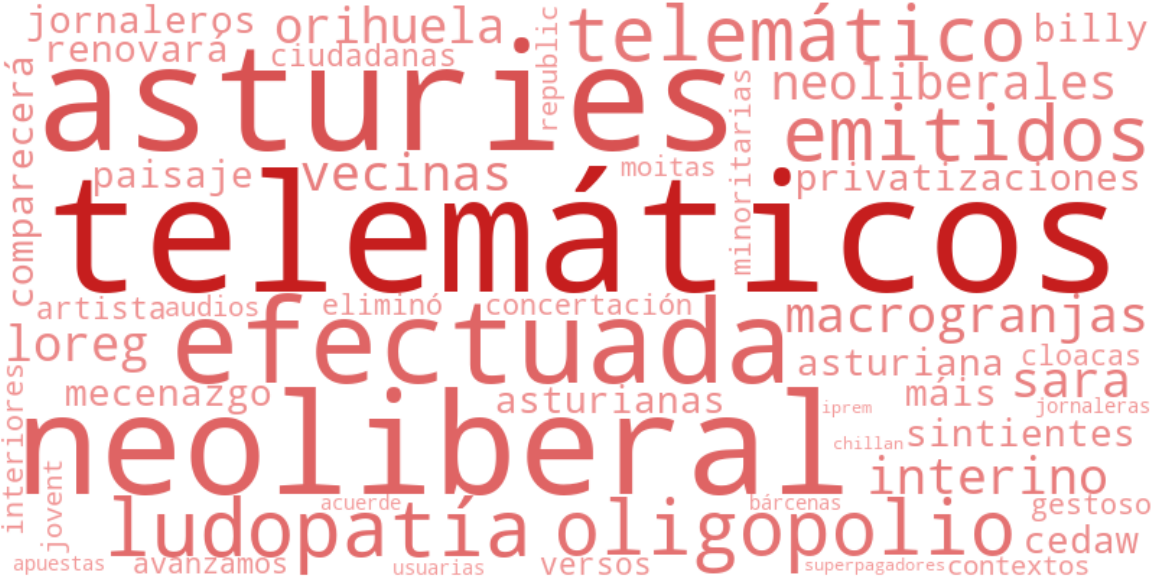
\includegraphics[width=\linewidth]{figures/congress_left.pdf}

		\end{minipage}
		\hspace{0.04\textwidth}
		\begin{minipage}{0.46\textwidth}
						\label{fig:worcloud2}
						\captionof{figure}{Word Cloud Top Right Words}
			\centering
			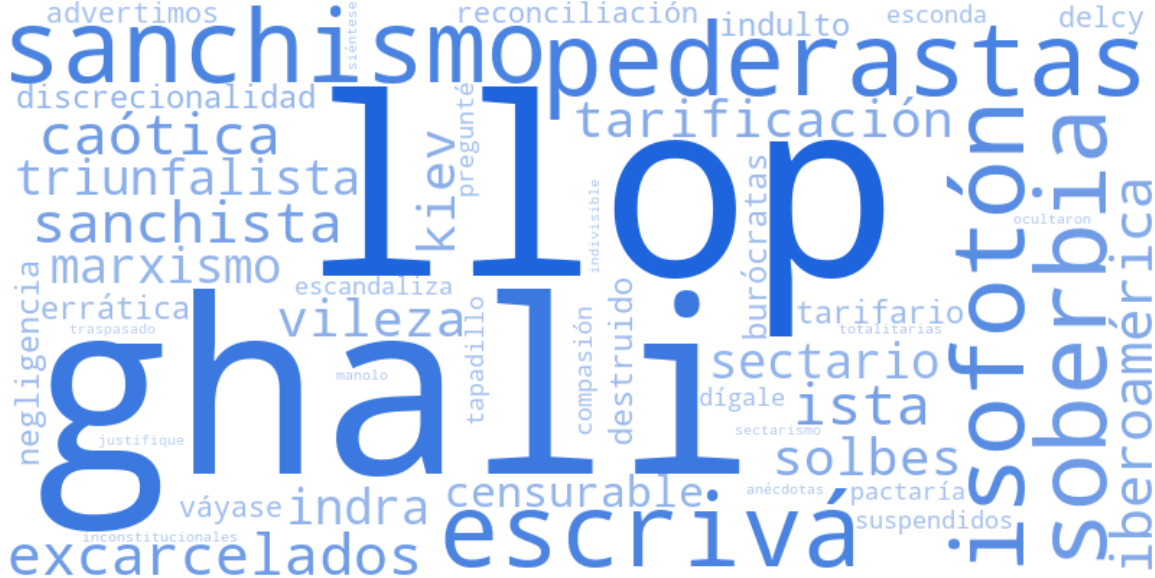
\includegraphics[width=\linewidth]{figures/congress_right.pdf}


		\end{minipage}
		\caption*{\small Notes: The wordclouds represent the Top Words with lowers (left) and highest (right) scores as defined in equation \ref{eq:log_ratio}. Size of the word is weighted by word frequency appearance.  }
	\end{figure}
	
	
	
	
	
	Finally, to classify the channel data, I calculate for each channel the fraction of tokens that appear in the left-coded list versus the right-coded list. This yields an index of ideological slant that reflects which side's language is more prevalent in the channel’s content. The 
	
	
	
	\begin{figure}[H]
		\centering
		\caption{Normalized Ideology Scores}
		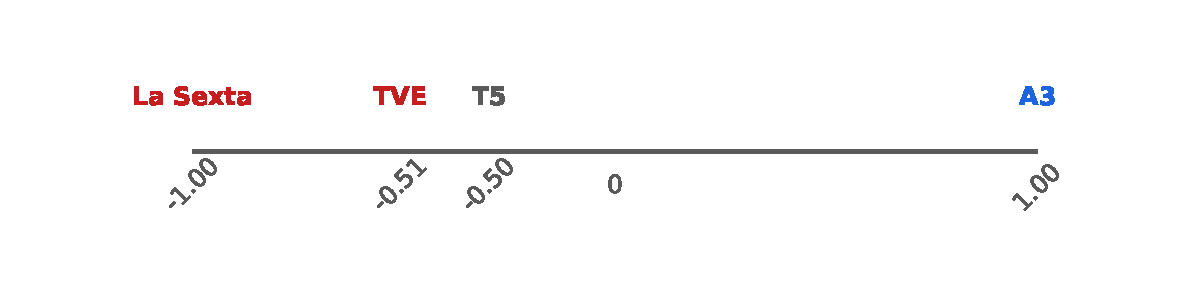
\includegraphics[width=120mm]{figures/congress_line}
		\caption*{\small Notes: The figure shows the normalized ideology positions of the channels after the text classification based on congress speeches. }
		\label{fig:congress_line}
	\end{figure}
	
	
	\begin{comment}
	
	
	 I apply a BERT sentence transformer to convert both sets (party speeches and channel texts) into numerical vectors. Finally, I use cosine similarity to compare each channel vector against each party vector, generating a similarity matrix where each cell indicates how close a channel’s content is to a party’s rhetoric. The results are shown in figure \ref{fig:congress}. 
	
	
	
	\begin{figure}[H]
		\centering
		\caption{Cosine similarity of congress speeches to outlet's content}
		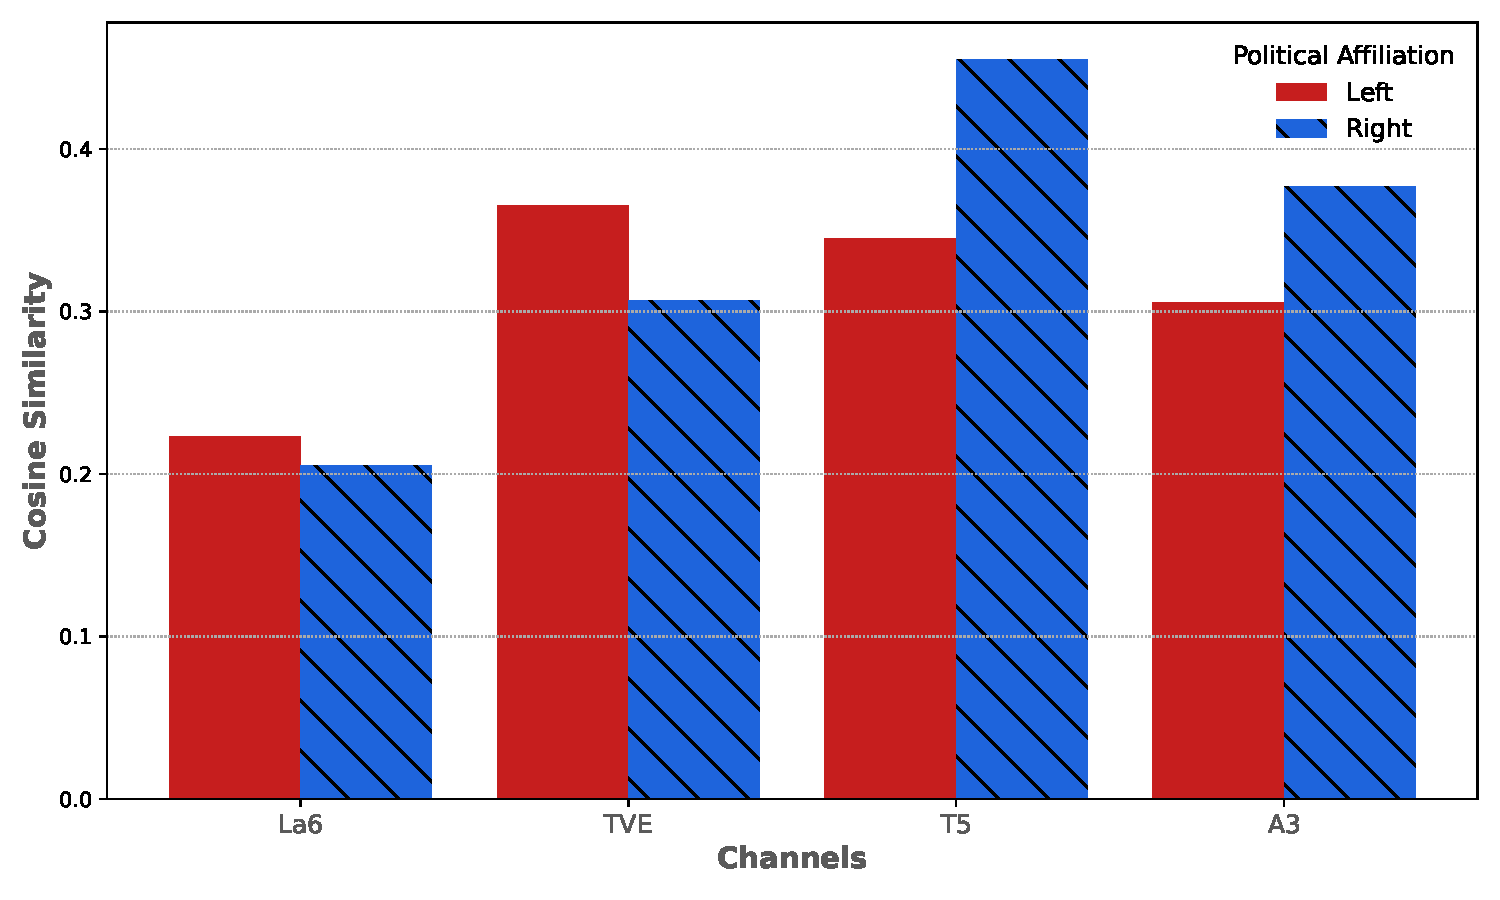
\includegraphics[width=120mm]{figures/congress}
		\caption*{\small Notes: The figure shows the percentage of stories to each political party for a given sentiment. We exclude neutral stories.}
		\label{fig:congress}
	\end{figure}
	
	
	\end{comment}
	
	
	
	
	
	
	
		\subsection{Instrument validity}
	
	
	The instrumental variable approach outlined in section \ref{section:endogeneity} relies on the assumption that the news landscape, proxied by the pool of stories, is a pure supply shifter. This assumption would be violated if viewers exhibit some anticipation behavior. Viewers naturally know that, for instance,  a scandal occurred; the assumption is that they cannot see is the volume and polarity of the raw wire material that the channels count on. As a diagnostic, I regress minute-0 audience shares on the available pool of stories on the same day. In this sense, these results serve as a falsification test where, if there was anticipation behavior, initial audience would tune into different channels according to the news landscape of that given day.
	
	\begin{equation}\label{eq:check_exogeneity}
		\begin{aligned}
			ln\left( \frac{q_{jt}}{L_{r}-Q_{jt}}  \right) = \beta_0 + \sum_{p \in \{L,R\}}\left(\rho^{p+} z^{p+}_d + \rho^{p-} z^{p-}_d \right)+ \phi z^{political}_d + \gamma_{dow} + \gamma_r + \epsilon_{jt}
		\end{aligned}
	\end{equation} 
	
	
	
	
	\begin{table}
		\centering
		{
\begin{tabular}{l*{4}{c}}
\hline
&\multicolumn{4}{c}{$   ln\left( \frac{q_{crd}}{L_{r}-Q_{rd}}  \right)$}\\
\hline
          &\multicolumn{1}{c}{(1)}&\multicolumn{1}{c}{(2)}&\multicolumn{1}{c}{(3)}&\multicolumn{1}{c}{(4)}\\
          \hline
\hline
pos\_right\_news&  -1.1830\sym{***}&  -1.2970\sym{***}&  -0.9093\sym{***}&  -0.9572\sym{***}\\
          & (0.2379)         & (0.2059)         & (0.2365)         & (0.2832)         \\
pos\_left\_news&   0.2434         &   0.8154\sym{***}&   0.6709\sym{***}&   0.6657\sym{***}\\
          & (0.2172)         & (0.1709)         & (0.2461)         & (0.2339)         \\
neg\_right\_news&  -0.6172\sym{***}&  -0.7594\sym{***}&  -1.0197\sym{***}&  -0.5473\sym{**} \\
          & (0.2177)         & (0.1771)         & (0.2712)         & (0.2548)         \\
neg\_left\_news&   1.5192\sym{***}&   1.7982\sym{***}&   1.0508\sym{***}&   1.0127\sym{***}\\
          & (0.2582)         & (0.2026)         & (0.2770)         & (0.2861)         \\
political\_news&  -0.5071\sym{**} &  -0.5051\sym{***}&   0.0565         &  -0.3992\sym{*}  \\
          & (0.2029)         & (0.1723)         & (0.2213)         & (0.2388)         \\
\_cons     &  -3.3131\sym{***}&  -2.7860\sym{***}&  -3.6418\sym{***}&  -4.1093\sym{***}\\
          & (0.0650)         & (0.0546)         & (0.0671)         & (0.0724)         \\
\hline
\(N\)     &     2231         &     2555         &     2001         &     2381         \\
\hline\hline
\multicolumn{5}{l}{\footnotesize Standard errors in parentheses}\\
\multicolumn{5}{l}{\footnotesize \sym{*} \(p<0.10\), \sym{**} \(p<0.05\), \sym{***} \(p<0.01\)}\\
\end{tabular}
}

		\caption{The table shows the results from the estimation of \ref{eq:check_exogeneity} conditional on minute 0 audience. Each column represents the regression on channels TVE, A3, Telecinco and La Sexta ; respectively. Day of the week and region fixed effects are included. }
		\label{table:check_exogeneity}
	\end{table}
	
	
	Table \ref{table:check_exogeneity} show the estimated coefficients from equation \ref{eq:check_exogeneity} where each column corresponds to a separate outlet regression and I condition on the minute zero audience. Equation \ref{eq:check_exogeneity} is the linear analogue of a logit estimation. The consistent sign of the coefficients across the different covariates indicates that viewers might not strategically choose across the outlets as a function of what the stories of the day were. This, however, doesn't preclude strategic substitution towards the outside option. 
	
	
	
	
	
	\subsection{Alternative methods for segment splitting in unstructured text}
	
	I explain here different unsupervised text splitting methods that were tried to split the segments of the day. To the best of my knowledge, these methods have not been applied before and can be easily extended to any TV news set up. The advantage of these techniques is that they provide an unsupervised way to split unstructured text into stories that is precise up to the second level, thus overcoming the problem of the manually annotated labels which goes at the minute level. There is, however, computational or financial costs in some of them that impeded me to use them for the whole dataset.
	
	\textbf{Image recognition}
	
	Outlets typically segment their sections by means of captions where they introduce headers for the upcoming story. Exploiting our video dataset, I designed an unsupervised image recognition algorithm that tracks the appearance of those new segments and produces a set of times that serve as text splitters. Although precise, the disadvantage of this method is that it remains computationally intensive as videos need to be segmented and then processed into the algorithm. Computational cost can be reduced by focusing on the lower bottom of the screen  only (figure \ref{figure:image_rec}), which is the area where the output is expected to appear.
	
	\begin{figure}[H]
		\centering
		\caption{Example of  image story delimiter}
		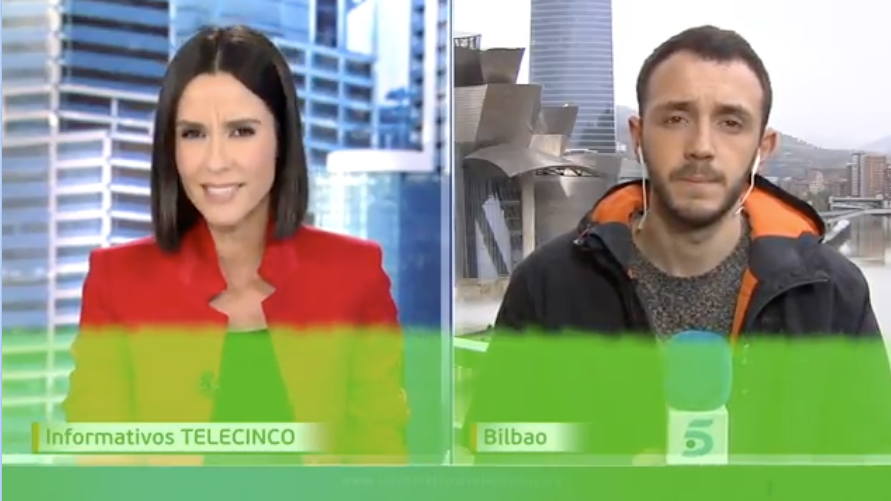
\includegraphics[width=100mm]{figures/image_recog}
		
		\caption*{\small Notes: Example of a image with a caption that delimits the beginning of a new section. The highlighted area shows the bottom of the image where image recognition can be applied to find such appearances.}
			\label{figure:image_rec}
	\end{figure} 
	
	
	
	
	\textbf{Speaker diarization}
	
	
	A less computationally expensive alternative consist on using \textit{speaker diarization} on the wav files. After transforming the mp4 file to audio using \textit{ffmpeg}, I use Google Cloud diarization tool to find the different speakers in an audio file. The most common (or most two common if it is a weekend) speakers overall corresponds to the presenter of the news. After allowing a flexible specification, one can identify break points by cheeking the seconds where the presenter comes back into scene making sure she is speaking long enough so that a new segment is being introduced. Figure \ref{fig:diarization} illustrates this procedure and the comparison with the manually annotated labels for an example day-channel.
	
	
	\begin{figure}[H]
		\centering
		\caption{Comparison audio splitting with annotated section splits}
		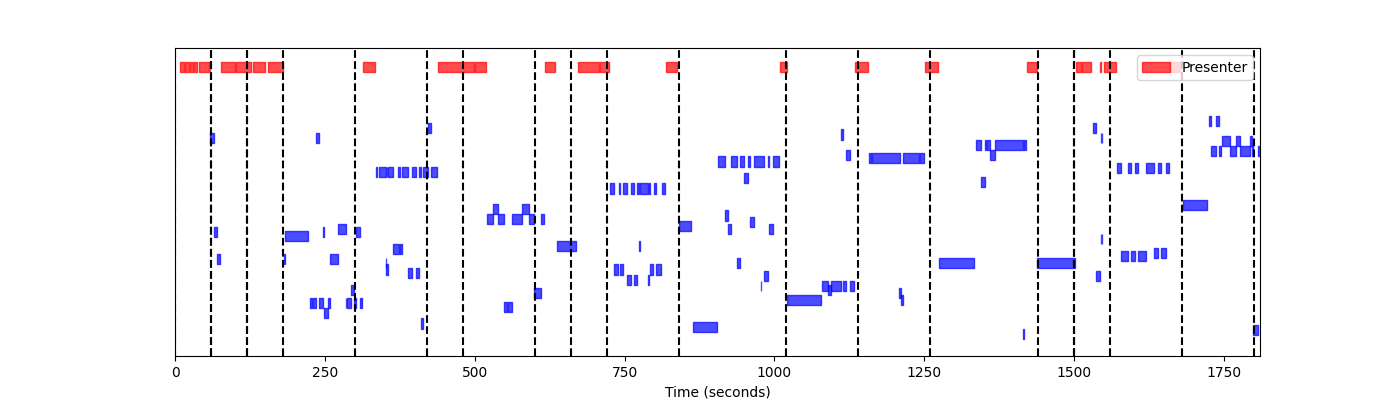
\includegraphics[width=120mm]{figures/speakers_all}
		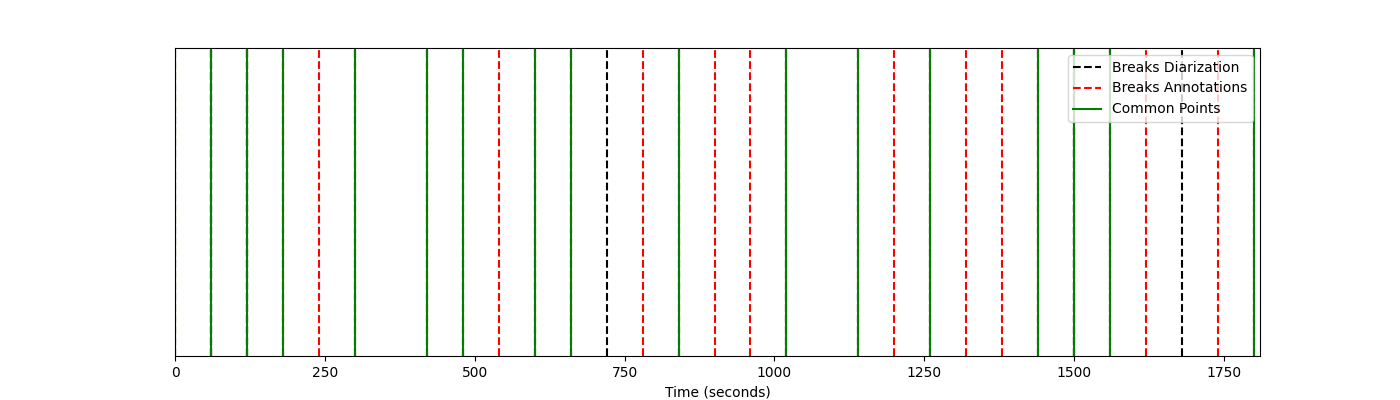
\includegraphics[width=120mm]{figures/speaker_timeline}
		\caption*{\small Notes: The top figure shows the timeline for the presenter audio (red) vs other audios recognized by \textit{speech2text} in a wav file for the 15th January 2023 in La Sexta. Vertical, black, dashed lines represent the predicted splits based on the diarization. The bottom figure combines these splits with the ones that come from the manually annotated figures. Red, dashed bars correspond to the breaks that come from the manually annotated GECA dataset. Green bars represent breaks where both the speaker diarization and the manual annotation coincide on a break. }
		\label{fig:diarization}
	\end{figure}
	
	
	
	
	
	
	
	
	
	
	
	%\nocite{*}
	\clearpage
	%\addcontentsline{toc}{chapter}{Bibliography}
	%\printbibliography
	
	\addcontentsline{toc}{chapter}{Bibliography}
	\bibliographystyle{apa}
	\bibliography{./bib/media_bias.bib}
	
	
	
	
	
	
	
	
	
	
	
	
\end{document}